\documentclass[10pt]{book}
\usepackage{0_Packages}
\usepackage{1_Environnements}
\usepackage{2_Commandes_gen}
\usepackage{2_Commandes_meca}

\pagestyle{plain}
\def\path{./fig}
\usepackage{natbib}
\bibliographystyle{abbrvnat}
\setcitestyle{authoryear,numbers,square}
\newcommand{\cv}{c_{v}}
\newcommand{\Cm}{C_{\mathrm{m}}}
\newcommand{\PsiVol}{U}
\newcommand{\vgrad}{\vec{\text{grad}}\,}
\newcommand{\MatMass}{\mathbb{M}}
\newcommand{\FLin}{\vec{f}^{\ell}}
\newcommand{\dlo}{\d\ell_{0}}
\newcommand{\npart}[1]{<#1>_{-}}
\newcommand{\Convexe}{\Cc}
\newcommand{\Gc}{\Gg_{c}}
\newcommand{\Int}[2]{\int_{#1}^{#2}}
\newcommand{\FthEpsp}{\ten{A}}

\begin{document}
\part{Théorie}\label{Part:Theorie}
\chapter*{Introduction}
La partie pratique achevée, nous précisons ici brièvement la théorie des modèles implémentés dans le code CHARON. Cette partie ne peut être considérée comme un traité de mécanique complet. Nous renverrons, le cas échéant le lecteur, à des ouvrages de référence dont sont tirées les lois ici utilisées.
\begin{itemize}[label=$\star$]
\item Dans un premier \chapref{Chapitre:Problème hydrodynamique}, les équations générales régissant les solides déformables sont présentées. Les transformations envisagées sont finies. 
\item Dans un deuxième \chapref{Chapitre:Modèles réduits}, sont étudiés les modèles bi-dimensionnels, (plan et axisymétrique), et uni-dimensionnel (plan, cylindrique et sphérique) vus comme des modèles dégénérés du système général proposé au chapitre précédent.
\end{itemize}
A ce stade, les lois de comportement reliant la contrainte actuelle de Cauchy aux paramètres de notre problème ne sont pas connues. Les chapitres suivants présentent un certain nombre de modèles de loi de comportement.
\begin{itemize}[label=$\star$]
\item Le comportement élastique, précédant systématiquement l'apparition d'autres phénomènes plus exotiques, est d'abord envisagé au \chapref{Chapitre:Équations d'état loi deviatorique}. Les lois d'états reliant la masse volumique, la température et la pression sont identifiées comme des lois élastiques et sont donc renseignées dans ce chapitre.
\item La plasticité dans le cadre des petites perturbations, puis étendue aux transformations finies, est abordée au \chapref{Chapitre:Plasticité}.
\item L'endommagement, par les modèles \og champ de phase \fg{}, mais aussi via les modèles de Johnson, est détaillé au \chapref{Chapitre:Endommagement}. Les modèles de Johnson sont actuellement privilégiés pour prédire la rupture des matériaux ductiles.
\item Un \chapref{Chapitre:Modèle multiphasique}, concernant la simulation de système multiphasique, conclut le corps principal de cette partie théorique. Il précise les capacités de CHARON à effectuer des simulations sur un solide constitué de plusieurs matériaux ou qui peut être sujet à des transitions de phase.
\item Des formulaires \Annexeref{Annexe:Formulaire} complètent la théorie en rejetant les difficultés et lourdeurs mathématiques en fin d'ouvrage.
\end{itemize}
\begin{DefNotations}{Notations générales}
\widecellh{2.5}{1.5}{$\SC$} & Tenseur des contraintes de Cauchy\\\hline
\widecellh{2.5}{1.5}{$\devia$} & Déviateur des contraintes de Cauchy\\\hline
\widecellh{2.5}{1.5}{$-p$} & Pression, opposée de la valeur moyenne des contraintes de Cauchy\\\hline
\widecellh{2.5}{1.5}{$\GT$} & Gradient de la transformation\\\hline
\widecellh{2.5}{1.5}{$\Dep$} & Champ de déplacement\\\hline
\widecellh{2.5}{1.5}{$\TD$} & Tenseur taux de déformation\\\hline
\widecellh{2.5}{1.5}{$\CGG$} & Tenseur de déformation de Cauchy-Green gauche\\\hline
\widecellh{2.5}{1.5}{$\DefoHPP$} & Déformation linéarisée\\\hline
\widecellh{2.5}{1.5}{$\TU$} & Tenseur métrique\\\hline
\widecellh{2.5}{1.5}{$\DepVirt$} & Champ test (déplacement virtuel)\\\hline
\widecellh{2.5}{1.5}{$\Configuration_{t}$} & Domaine actuel d'étude\\\hline
\widecellh{2.5}{1.5}{$\dNOm$} & Frontières pour les conditions aux limites en efforts\\\hline
\widecellh{2.5}{1.5}{$\dDOm$} & Frontières pour les conditions aux limites en déplacements\\\hline
\widecellh{2.5}{1.5}{$\J$} & Dilatation volumique actuelle\\\hline
\widecellh{2.5}{1.5}{$\rho$} & Masse volumique actuelle\\\hline
\end{DefNotations}
\chapter{Problème mécanique}\label{Chapitre:Problème hydrodynamique}
\section*{\emph{Introduction}}
Nous n'envisageons ici que la mécanique dans le cadre traditionnel de Cauchy. La seule variable cinématique retenue, caractérisant supposément complètement le mouvement de notre milieu continu, est le champ de déplacement tridimensionnel $\Dep$.
\begin{itemize}
\item Nous commençons \secref{Section:Équations générales du problème mécanique} par rappeler les principes et équations fondamentales tridimensionnelles dans le cadre de la mécanique de Cauchy.
\item La formulation intégrale, ramenée sur la configuration de référence sera ensuite abordée à la \secref{Section:Formulation en grandes transformations du problème mécanique}. Cette formulation intégrale est la forme mathématiques fondamentale d'entrée du code CHARON
\item La résolution séquentielle du problème d'évolution est abordée à la \secref{Section:Stratégie incrémentale de résolution, algorithme de dynamique explicite}. Nous y esquissons les grandes phases du schéma de \og dynamique explicite \fg{}.
\end{itemize}
\section{Équations générales du problème mécanique}\label{Section:Équations générales du problème mécanique}
\subsection{Principe fondamental de la dynamique, équation du mouvement}
\begin{Hypothese}{Force de volume négligeable} Nous négligeons dans la suite l'action des forces de volume dont la faible magnitude n'apporte pas de correction significative aux résultats obtenus.
\end{Hypothese}
Les équations d'équilibre, dans le cadre de la mécanique des milieux continus de Cauchy, sont posées sur la configuration actuelle:
\begin{equation}
\begin{aligned}
\vdiv_{E}\SC=\rho\dfrac{\partial^{2} \Dep}{\partial t^{2}} \sur \Configuration_{t}
\end{aligned}
\label{eq:equilibre}
\end{equation}
Ces équations, valables sur l'ensemble du domaine matériel à l'étude $\Configuration_{t}$, sont complétées par des conditions aux limites de Neumann et de Dirichlet, aussi appelées \og conditions aux limites en effort et en déplacement \fg{} respectivement:
$$\SC\cdot\NormaleAct=\vec{T}^{D} \sur \dNOm \et \Dep=\Dep^{D} \sur \dDOm$$
avec les conditions de complémentarité et d'exclusion:
$$ \dNOm \cup \dDOm = \partial\Configuration_{t}; \quad \dNOm \cap \dDOm = \emptyset$$
\subsection{Principe de conservation de l'énergie, équation de la chaleur}
L'énergie interne vérifie l'équation \og de la chaleur \fg{}, traduisant la conservation locale de l'énergie. Plus précisément, la dérivée temporelle de l'énergie interne massique $\EIntMass$ satisfait:
\begin{equation}
\rho\dot{e}^{m}=\SC:\TD+\PCaloVol-\div_{E}\CourantChal
\label{eq:chaleur}
\end{equation}
Avec les notations usuelles $\PCaloVol$ désigne l'apport volumique de chaleur d'origine extérieure, $\CourantChal$ le vecteur densité de courant de chaleur complété par une loi de comportement thermique.

La puissance volumique d'origine extérieure sera essentiellement de deux natures:
$$\PCaloVol=\mathscr{P}_{vol}^{ray}+\mathscr{P}_{vol}^{chim}$$
\begin{itemize}
\item Une puissance volumique déposée par rayonnement $\mathscr{P}_{vol}^{ray}$.
\item Une puissance volumique calorifique d'origine chimique due à des transitions de phase $\mathscr{P}_{vol}^{chim}$ liée à l'évolution de la concentration. Si l'on note $e_{p}^{m}$ l'énergie massique libérée par la production d'une unité de masse de produit, $c_{p}$ la concentration du produit, et $\rho_{p}$ la masse volumique du produit, la puissance volumique calorifique d'origine chimique $\mathscr{P}_{vol}^{chim}$ s'écrit:
\begin{equation}
\mathscr{P}_{vol}^{chim} =\sum_{p} \dot{c}_{p}\rho_{p}e_{p}^{m}=\dfrac{\d\mathscr{E}_{vol}^{chim}}{\dt}
\label{eq:prod_origine_chimique}
\end{equation}
En pratique, dans le code CHARON la puissance produite d'origine chimique est calculée de manière incrémentale:
\begin{equation}
\mathscr{P}_{vol}^{chim} =\sum_{p} \dfrac{(c_{p}^{n+1}-c_{p}^{n})e_{p}^{vol}}{\Delta t}
\label{eq:prod_origine_chimique_incremental}
\end{equation}
où $e_{p}^{vol}$ désigne une énergie libérée par unité de volume. $[e_{p}^{vol}]=\joule.\metre^{-3}=\kilo\gram\metre^{-1}\second^{-2}$, autrement dit $e_{p}^{vol}$ est homogène à une contrainte.
\end{itemize}
\subsubsection{Cas particulier de l'évolution adiabatique}
\begin{Hypothese}{Évolutions adiabatiques} Nous annulons, dans une première étude, les transferts thermiques.
\end{Hypothese}
L'équation de la chaleur se simplifie par conséquent:
\begin{equation}
\rho\dot{e}^{m}=\SC:\TD+\PCaloVol
\label{eq:chaleur_hyp}
\end{equation}
Nous postuler que nous pouvons relier la variation d'énergie interne massique et de température par l'intermédiaire d'une capacité thermique massique tangente $C^{m}_{tan}$:
\begin{equation}
\dot{e}^{m}=C^{m}_{tan}(\Dep,T)\dot{T}
\label{eq:rel_dot_e_dot_T}
\end{equation}
Ce qui nous donne en l'équation différentielle temporelle portant sur le champ de température en combinant \eqref{eq:prod_origine_chimique}, \eqref{eq:chaleur_hyp} et \eqref{eq:rel_dot_e_dot_T}:
$$\rho C^{m}_{tan}(\Dep,T)\dot{T} = \SC:\TD +\dot{c}_{p}\rho_{p}e_{p}^{m}$$
Dans le cas simple d'une évolution adiabatique sans terme de rayonnement, la température est par conséquent actualisée à chaque incrément par le schéma explicite:
$$T_{n+1}=T_{n}+\Delta T \avec \Delta T =\dfrac{\SC:\TD\Delta t+\Delta c_{p}\rho_{p}e_{p}^{m}}{C_{tan}} \et C_{tan}=\rho C^{m}_{tan}((\Dep_{n},T_{n})$$
avec $C_{tan}$ la capacité thermique volumique tangente.
\subsubsection{Cas générale avec une loi de comportement thermique linéaire}
Si nous ôtons l'hypothèse adiabatique, l'équation de chaleur prend habituellement le nom d'\og équation de diffusion \fg{}. Tout comme le problème mécanique doit être fermé par une loi de comportement reliant la contrainte $\SC$ au champ de déplacement $\Dep$, le flux de chaleur $\vec{q}$ doit être mis en relation avec le champ de température.

Nous supposons que la loi de comportement thermique est linéaire (loi de Fourier) et qu'il existe une capacité thermique tangente, fonction de l'état au pas $n$. Alors l'équation de la chaleur s'écrit sous forme symbolique:
\begin{equation}
\rho C^{m}_{tan}((\Dep_{n},T_{n})\dfrac{T_{n+1}-T_{n}}{\Delta t}=\SC(T_{n},\Dep_{n}):\TD(T_{n},\Dep_{n})+\PCaloVol-\div_{E}\left(\lambda\vgrad_{E} T_{n+1}\right)
\label{eq:chaleur}
\end{equation}
Notons $\hat{T}$ le champ test de température (température virtuelle) alors le problème tridimensionnel \eqref{eq:chaleur} peut se réécrire sous forme intégrale:
$$\int_{\Dmt}\dfrac{C_{tan}(\Dep_{n},T_{n})}{\Delta t}T_{n+1}\hat{T}+\lambda \vgrad_{E}T_{n+1}\cdot\vgrad_{E}\hat{T}\dvt=\int_{\Dmt}\dfrac{C_{tan}(\Dep_{n},T_{n})}{\Delta t}T_{n}\hat{T}+\SC:\TD \dvt$$
Ce problème variationnel peut ensuite être résolu par la méthode des éléments finis standard.
\subsection{Équation locale de conservation de la masse}
La masse volumique $\rho$ locale satisfait l'équation de conservation de la masse, laquelle peut s'écrire sous forme condensée:
\begin{equation}
\rho= \dfrac{\rho_{0}}{\det\GT}=\dfrac{\rho_{0}}{\det\left(\TU+\tgrad_{L}\Dep\right)}
\label{eq:conserv_mass}
\end{equation}
où $\GT$ désigne le gradient de la transformation. Cette équation algébrique ne sert qu'à l'actualisation de la masse volumique actuelle $\rho$ et n'a pas besoin d'être résolue dans la mesure où elle est implicitement prise en compte dans la formulation du problème.
\subsection{Second principe de la thermodynamique}
Le second principe de la thermodynamique se traduit par une inéquation différentielle relative à la croissance de l'entropie d'origine interne au cours de l'évolution. Cette équation n'est jamais résolue explicitement dans les problèmes de mécanique du solide car les lois de comportement reliant les contraintes aux inconnues principales du problème sont choisies de sorte à satisfaire automatiquement cette inégalité.
\section{Formulation en grandes transformations du problème mécanique}\label{Section:Formulation en grandes transformations du problème mécanique}
La résolution du problème mécanique repose sur la recherche d'une solution aux équations aux dérivées partielles d'équilibre \eref{eq:equilibre}, posées sur la configuration actuelle inconnue. Dans l'hypothèse des petites perturbations, classiquement employée en mécanique du solide, cette configuration actuelle est confondue avec la configuration de référence pour l'évaluation des sollicitations. Cette simplification s'avère féconde si les déformations et les rotations demeurent faibles. Toutefois, dans les problèmes caractéristiques au CEA-DAM, des déformations importantes rendent inenvisageable la simplification de l'hypothèse des petites perturbations et appelle un formalisme en grandes transformations. Ce formalisme embrasse deux grandes classes de procédé: 
\begin{itemize}
\item Les méthodes dites par \og Lagrangien actualisé \fg{}, qui résolvent le calcul incrémental en le considérant comme une succession de problèmes en petites perturbations. La configuration de référence étant, à chaque incrément, prise comme la dernière configuration actuelle obtenue.
\item Les méthodes \og Lagrangien total \fg{}, qui transportent l'ensemble des équations du problème sur la configuration de référence, connue.
\end{itemize}
La première méthode est habituellement privilégiée par les mécaniciens des fluides pour lesquels la notion de configuration de référence est peu significative, tandis que les mécaniciens des solides accordent plus de valeurs au Lagrangien total. Pour notre étude, nous retiendrons cette seconde mise en forme.\\

Contrairement à ce qui est parfois incorrectement affirmé, \emph{nul champ n'est par essence lagrangien ou eulérien}, car ces deux termes réfèrent à \emph{un choix de représentation}. La représentation Eulérienne consiste à paramétrer les champs dans la configuration actuelle et à se donner le champ des vitesses. La représentation Lagrangienne consiste à paramétrer les champs par rapport à la configuration de référence et à se donner la transformation $\Transfo$ qui relie bijectivement un vecteur $\PosInit$ de la configuration de référence à son \og transporté dans la configuration actuelle \fg{} $\PosAct$ .\\

Ainsi la contrainte de Cauchy $\SC$, souvent qualifiée \og d'Eulérienne \fg{} est un champ défini en tout point $P$ du solide que l'on peut noter $\SC(P,t)$. Il est possible de lui associer une représentation Eulérienne ou Lagrangienne:
$$\SC(P,t)=\SC_{E}(\PosAct,t)=\SC_{L}(\PosInit,t)$$
Pour plus de précision à cet égard, nous renvoyons le lecteur à \cite{garrigues2016algebre, garrigues2016cinematique}.\\

Dans la suite, les sous script $_{L}$, $_{E}$ référeront au type de représentation utilisée. Par extension, concernant les opérateurs différentiels, $\div_{E}$ correspondra par exemple à la divergence de la représentation eulérienne d'un champ, tandis que $\tgrad_{L}$ désignera le gradient de la représentation de Lagrange d'un champ vectoriel.
\subsection{Équations intégrales posées sur la configuration de référence}
La résolution par la méthode des éléments finis d'une équations aux dérivées partielles repose sur une formulation intégrale des équations \og fortes \fg{}. Cette formulation est obtenue en dualisant les équations par un champ test $\DepVirt$ inconnu puis en intégrant sur le domaine.\\

La formulation intégrale de l'équation d'équilibre \eref{eq:equilibre}, posée sur le domaine actuel $\Configuration_{t}$ est:
$$-\int_{\Configuration_{t}}\SC:\tgrad_{E}\DepVirt\dvt+\int_{\dNOm}\FSurf\cdot\DepVirt\dst=\int_{\Configuration_{t}}\rho\dfrac{\partial^{2}\Dep}{\partial t^{2}}\cdot\DepVirt\dvt$$
Le domaine d'intégration peut être ramené dans le configuration de référence par (voir \cite{garrigues2016cinematique} concernant les formules de transport):
\begin{equation}
\begin{aligned}
&-\int_{\Configuration_{0}}\SC_{L}:\left(\tgrad_{L}\DepVirt\cdot\GT^{-1}\right)\det\GT\dvo+\int_{\dNOm_{0}}\FSurf\cdot\DepVirt\Vert\GT^{-\top}\cdot\NormaleInit\Vert\det\GT\dso\\
&\qquad =\int_{\Configuration_{0}}\rho\dfrac{\partial^{2}\Dep}{\partial t^{2}}\cdot\DepVirt\det\GT\dvo  \avec \GT=\TU+\tgrad_{L}\Dep
\end{aligned}
\label{eq:forme_faible_config_ref}
\end{equation}
La dernière intégrale peut en outre se simplifier, en vertu du principe de conservation de la masse:
\begin{equation}
\int_{\Configuration_{0}}\rho\dfrac{\partial^{2}\Dep}{\partial t^{2}}\cdot\DepVirt\det\GT\dvo=\int_{\Configuration_{0}}\rho_{0}\dfrac{\partial^{2}\Dep}{\partial t^{2}}\cdot\DepVirt\dvo
\label{eq:simplification_forme_mass}
\end{equation}
Si bien que la formulation intégrale du problème prend, en définitive, la forme suivante:
\begin{equation}
-\int_{\Configuration_{0}}\SC_{L}:\left(\tgrad_{L}\DepVirt\cdot\GT^{-1}\right)\det\GT\dvo+\int_{\dNOm_{0}}\FSurf\cdot\DepVirt\Vert\GT^{-\top}\cdot\NormaleInit\Vert\det\GT\dso=\int_{\Configuration_{0}}\rho_{0}\dfrac{\partial^{2}\Dep}{\partial t^{2}}\cdot\DepVirt\dvo
\label{eq:forme_faible_config_ref_finale}
\end{equation}
La loi de comportement à ce stade n'est pas précisée et constitue l'objet de chapitres dédiés.
\begin{Defi}{Déformations conjuguées} Nous appelons déformation conjuguée à la représentation Lagrangienne de la contrainte de Cauchy $\SC_{L}$ le terme $\left(\tgrad_{L}\DepVirt\cdot\GT^{-1}\right)\det\GT$.
\end{Defi}
Cette déformation conjuguée peut se réécrire en introduisant la transposée de la comatrice de $\GT$ (appelée \emph{co-facteur} dans la littérature anglo-saxonne)\footnote{La définition du cofacteur ne semble pas faire l'unanimité. Pour \cite{hesch2017framework} il s'agit de: $\Cof\GT=\det(\GT)\GT^{-\top}$ tandis qu'en accord avec la définition du langage UFL 
%\url{https://fenics.readthedocs.io/projects/ufl/en/latest/manual/form_language.html?highlight=cofac#cofac} 
$\Cof\GT=\det(\GT) \GT^{-1}$}
\begin{equation}
\left(\tgrad_{L}\DepVirt\cdot\GT^{-1}\right)\det\GT=\tgrad_{L}\DepVirt\cdot\Cof\left(\GT\right)
\label{eq:defo_conjug_cofac}
\end{equation}
La formulation faible proposée \eqref{eq:forme_faible_config_ref_finale} est originale, elle ramène les grandeurs sur la configuration de référence ($\Configuration_{0}$) connue tout en conservant la contrainte de Cauchy comme mesure de la contrainte. Elle permet donc l'utilisation de lois de comportement définies sur la configuration \og actuelle \fg{} telles que des lois d'état (voir \secref{Section:Loi d'état})
\section{Stratégie incrémentale de résolution, algorithme de dynamique explicite}\label{Section:Stratégie incrémentale de résolution, algorithme de dynamique explicite}
Si nous supposons connu au temps $t_{k}$ l'ensemble des champs mécaniques, nous résolvons séquentiellement:
\begin{itemize}
\item Résolution de l'équation du mouvement \eqref{eq:equilibre} -> $\Dep_{k+1}$
\item calcul de l'énergie interne à partir de \eqref{eq:chaleur} -> $\EIntMass_{k+1}$ 
\item actualisation de la valeur du champ de masse volumique via \eqref{eq:conserv_mass}, 
\item actualisation de la loi de comportement \eqref{eq:Loi_compo_gen}
\end{itemize}
Nous obtenons alors l'ensemble des champs au pas $k+1$ et initions un nouveau pas de calcul.

%\begin{algorithm}[ht!]
%\Entree{Maillage, paramètres physiques et géométriques, chargement $\Dep^{D}$, $\vec{T}^{D}$}
%Découpage du chargement en $N$ pas $\Dep^{D}_{n}$, $\vec{T}^{D}_{n}$\\
%\Pour{$n\in\{1,\ldots,N\}$}{
%\Entree{$\Dep_{k}$, $e_{k}$, $\rho_{k}$, $\SC_{k}$}
%%\tcc*[f]{compteur de l'itération}\\
%Résolution en déplacement \eqref{eq:equilibre}, algorithme explicite\\
%\Sortie{$\Dep_{k+1}$}
%%\tcc*[f]{initialisation de l'endommagement}
%%\Tq{evol}{
%\Entree{$\Dep_{k}$, $\EIntMass_{k}$, $\rho_{k}$, $\SC_{k}$}
%Résolution équation chaleur \eqref{eq:chaleur}\\
%\Sortie{$\EIntMass_{k+1}$}
%%\Entree{Endommagement  déplacement }
%%Résolution du problème d'endommagement.\\
%%\Sortie{Predicteur d'endommagement }
%%\Pour{toute interface}{
%\Entree{$\Dep_{k+1}$}
%Actualisation de la masse volumique \eqref{eq:conserv_mass}\\
%\Sortie{$\rho_{k+1}$}
%\Entree{$\EIntMass_{k+1}$, $\rho_{k+1}$}
%Actualisation loi de comportement \eqref{eq:Loi_compo_gen}\\
%\Sortie{$\SC_{k+1}$}
%}
%%\eSi{$\Vert\Vert<Tol$}{$evol=False$}{$evol=True$, $k+=1$}
%%}
%%}
%\caption{\bf Résolution hydrodynamique}
%\label{algo:delam_algo}
%\end{algorithm}
Le schéma temporelle est le schéma d'ordre 2 classique de la dynamique explicite (voir \cite{bonnet2007analyse});
\paragraph{Condition CFL} L'utilisation d'un schéma dynamique explicite requiert un pas de temps soit inférieur à une valeur critique (condition de Courant-Freidrich-Levy). Habituellement, cette borne supérieure du pas de temps est estimée en début de simulation seulement car les déformations restent contenues et la distorsion des éléments faibles. Cependant, dans l'éventualité de larges déformations, il peut être nécessaire d’actualiser la condition CFL au cours du calcul. 
\subsection{Condensation de la matrice de masse, précaution particulière}
L'implémentation de l'algorithme de dynamique explicite requiert à chaque itération l'inverse de la matrice de masse $\MatMass$. Cette opération exige une expression simple de $\MatMass$ permettant son inversion explicite (idéalement $\MatMass$ serait diagonale). Les procédures dites \og de condensation \fg{} visent précisément à proposer une approximation diagonale de la matrice de masse, généralement en \og condensant \fg{} aux nœuds de l’élément, l'ensemble de sa masse.\\

Pour illustrer cette procédure, considérons un unique élément 1D à interpolation linéaire. Cet élément possède seulement deux nœuds et il est naturel d'affecter la moitié de la masse total de l’élément à chacune des extrémités. Appliquée à la formulation intégrale \eqref{eq:simplification_forme_mass} présentée précédemment, cela traduit l'approximation suivante:
$$\int_{0}^{L}\rho\ddot{\Dep}\cdot\DepVirt\det\GT(\Dep)\dxo\approx \dfrac{L}{2}\left[\left(\rho\ddot{\Dep}\cdot\DepVirt\det\GT(\Dep)\right)(0)+\left(\rho\ddot{\Dep}\cdot\DepVirt\det\GT(\Dep)\right)(L)\right]$$
Cette intégration peut être vu comme une intégration numérique de Gauss-Lobatto \cite{durufle2009influence, teukolsky2015short}.\\

Un problème se pose toutefois dans le cas des modèles axisymétrique, cylindrique et sphérique si jamais un nœud se trouve sur l'axe de symétrie car dans ce cas l'évaluation de l'intégrale sur l'axe de symétrie s'annule
$$\int_{0}^{R}\rho u_{r}\hat{w}_{r}\det\GT(\Dep)r\dr\approx \dfrac{1}{2}\left[\underbrace{\left(r\rho u_{r}\hat{w}_{r}\det\GT(\Dep)\right)(0)}_{=0}+\left(\rho u_{r}\hat{w}_{r}\det\GT(\Dep)\right)(R)\right]$$
\begin{Rem}{\label{Rem:erreur_matrice_condensee}La matrice de masse condensée par cette procédure possède donc des termes nuls et ne peut être inversée. Actuellement, le code CHARON exige que l'utilisateur décale d'une petite quantité les nœuds du maillage se trouvant sur l'axe, puis bloque leur mouvement radial.}\end{Rem}
\section{Système d'unité cohérent}\label{Section:Système d'unité cohérent}
Le code CHARON ne considère pas de système d'unité particulier. Les grandeurs doivent dont être renseignées avec cohérence (dénomination anglo-saxonne \og consistent-unit \fg{}). Nous rappelons dans le tableau suivant un certain nombre de ces systèmes\footnote{Voir quelques systèmes consignés dans \url{https://www.dynasupport.com/howtos/general/consistent-units}}:
\begin{table}[h!]
\centering \begin{tabular}{lllllllll}\hline
masse & longueur & temps & force & contraintes & énergie & densité & $C_{th}$ massique & Label\\
\kilo\gram & \metre & \second & \newton & \pascal & \newton.\metre & $\kilo\gram.\metre^{-3}$ & $\metre^{2}.\second^{-2}.\kelvin^{-1}$  & (1)\\
\gram & \milli\metre & \milli\second & \newton & \mega\pascal & \newton\cdot\milli\metre & $\gram.\milli\metre^{-3}$ & $\milli\metre^{2}.\milli\second^{-2}.\kelvin^{-1}$ & (2)\\
\end{tabular}
\end{table}\\
Le système (2) est obtenu en remarquant que par exemple si le module d'Young était de $210\times 10^{9}\pascal$ alors:
$$210\times 10^{9}\pascal = 210\times 10^{9}\kilo\gram.\metre^{-1}.\second^{-2}=210\times 10^{12}\gram.\metre^{-1}.\second^{-2} = 210\times 10^{9}\gram.\milli\metre^{-1}.\second^{-2}= 210\times 10^{3}\gram.\milli\metre^{-1}.\milli\second^{-2}$$
Pour un acier standard, on a ainsi les ordres de grandeurs suivants:
\begin{table}[h!]
\centering \begin{tabular}{lllllllll}\hline
$E$ & $\rho$ & $C_{th}$ massique & $\alpha$ & Label\\
$2.07\times 10^{11}\pascal$ & $7.83\times 10^{3}\kilo\gram.\metre^{-3}$ & $500\metre^{2}.\second^{-2}.\kelvin^{-1}$ & $12\times 10^{-6}\kelvin^{-1}$ & (1)\\
$2.07\times 10^{5}\mega\pascal$ & $7.83\times 10^{-3}\gram.\milli\metre^{-3}$ & $500\milli\metre^{2}.\milli\second^{-2}.\kelvin^{-1}$ & $12\times 10^{-6}\kelvin^{-1}$ & (2)\\
$2.07\times 10^{5}\mega\pascal$ & $7.83\times 10^{-9}\ton.\milli\metre^{-3}$ & $500\times 10^{6}\milli\metre^{2}.\second^{-2}.\kelvin^{-1}$ & $12\times 10^{-6}\kelvin^{-1}$ & (3)\\\hline
\end{tabular}
\end{table}
\\

Pour obtenir des expressions dont l'ordre de grandeurs est raisonnable, nous suggérons à l'utilisateur d'utiliser le système numéro (2).
\chapter{Modèles réduits}\label{Chapitre:Modèles réduits}
\section*{\emph{Introduction}}
La pratique expérimentale repose sur un certain nombre d’expériences élémentaires, géométriquement simples, et servant à valider tout ou partie d'un modèle mécanique complexe. Pour reproduire numériquement ces expériences, l'usage consacre des modèles réduits, qui ne sont que des simplifications quantitativement acceptables du modèle tridimensionnel. Pour obtenir ces modèles réduit, le cas tridimensionnel est augmenté d'hypothèses cinématiques supplémentaires afin de simplifier la résolution. 
\begin{itemize}[label=$\star$]
\item Nous présentons d'abord, \secref{Section:Modèle bidimensionnel}, les modèles réduits bidimensionnels qui incluent les problèmes plans et à symétrie de révolution autour d'un axe. Ce dernier est d'un intérêt certain car il permet de représenter sobrement la dynamique des cylindres.
\item Nous détaillons ensuite à la \secref{Section:Modèles unidimensionnels} les modèles réduits unidimensionnels qui englobent les modèles cartésien 1D, cylindrique et sphérique. 
\end{itemize}
La formulation intégrale des équations d'équilibres, ramenée sur la configuration de référence, a été donnée dans le cas tridimensionnel à l'\eref{eq:forme_faible_config_ref_finale}:
\begin{equation}
-\int_{\Configuration_{0}}\SC_{L}:\left(\tgrad_{L}\DepVirt\cdot\GT^{-1}\right)\det\GT\dvo+\int_{\dNOm_{0}}\FSurf\cdot\DepVirt\Vert\GT^{-\top}\cdot\NormaleInit\Vert\det\GT\dso=\int_{\Configuration_{0}}\rho_{0}\dfrac{\partial^{2}\Dep}{\partial t^{2}}\cdot\DepVirt\dvo
\label{eq:rappel_formulationvariationnelle_3D}
\end{equation}
L'enjeu de ce chapitre consiste à préciser comment cette formulation intégrale, posée sur le domaine de référence $\Configuration_{0}$, peut être simplifiée au regard d'hypothèses cinématiques supplémentaires.
\section{Modèle bidimensionnel}\label{Section:Modèle bidimensionnel}
Dans cette section, nous précisons quelques simplifications consécutives à l'approximation \og bi-dimensionnel du problème \fg{}. Nous supposons que le champ de déplacement inconnu n'est fonction que de deux variables et n'est porté qui suivant deux vecteurs. Cette hypothèse recouvre par conséquent les problèmes dits plans (contraintes et déformations planes) ainsi que les modèles axi-symétrique. Les contraintes héritent des mêmes dépendances en fonctions des champs mécanique. Le champ de déplacement simplifié induit un champ de déformation et également de déformation conjugué plus simple.
\subsection{Modèle bi-dimensionnel plan}\label{Subsection:Modèle bi-dimensionnel plan}
\begin{Hypothese}{Problème plan} Dans un repère cartésien orthonormé, nous postulons la dépendance suivante du champ de déplacement:
$$\vec{u}=u_{x}(x,y)\ex+u_{y}(x,y)\ey$$
\end{Hypothese}
Nous désignons par \og modèle en déformation plane \fg{} le jeu d'équations découlant de cette hypothèse cinématique. Nous ne considérons ici que des grandeurs défini dans le plan $(Oxy)$ et réduisons les champs tridimensionnels à ce plan en les accompagnant de l'indice \og $_{2}$ \fg{} Le gradient du champ de déplacement et de la transformation s'écrivent:
$$\tgrad_{L2}\Dep=\begin{pmatrix}
\partial_{x}u_{x} & \partial_{y}u_{x}\\
\partial_{x}u_{y}  & \partial_{y}u_{y}\\
\end{pmatrix} \implique \GT_{2} = \begin{pmatrix}
1+\partial_{x}u_{x} & \partial_{y}u_{x}\\
\partial_{x}u_{y}  & 1+\partial_{y}u_{y}\
\end{pmatrix}$$
L'inverse du gradient de la transformation est simplement:
$$\GT_{2}^{-1} = \dfrac{1}{\left(1+\partial_{y}u_{y}\right)\left(1+\partial_{x}u_{x}\right)-\partial_{y}u_{x}\partial_{x}u_{y}}\begin{pmatrix}
1+\partial_{y}u_{y} & -\partial_{y}u_{x}\\
-\partial_{x}u_{y} & 1+\partial_{x}u_{x}\\
\end{pmatrix}$$
Avec ces hypothèses la formulation variationnelle tridimensionnelle \eqref{eq:rappel_formulationvariationnelle_3D} se résume à:
$$-\int_{\mathscr{S}_{0}}\SC_{2L}:\left(\tgrad_{2L}\DepVirt\cdot\GT_{2}^{-1}\right)\det\GT_{2}\dso+\int_{\mathscr{S}_{0}^{N}}\FLin_{L}\cdot\DepVirt\Vert\GT^{-\top}_{2}\cdot\NormaleInit\Vert\det\GT_{2}\dlo=\int_{\mathscr{S}_{0}}\rho_{0}\dfrac{\partial^{2}\Dep}{\partial t^{2}}\cdot\DepVirt\dso$$
Le problème mécanique ne dépend alors que de deux variables d'espace. En introduisant, le cofacteur comme définie à l'équation \eref{eq:defo_conjug_cofac}, nous obtenons en définitive la formulation faible implémentée dans le code CHARON:
\begin{equation}
-\int_{\mathscr{S}_{0}}\SC_{2L}:\left(\tgrad_{2L}\DepVirt\cdot\Cof\GT_{2}\right)\dso+\int_{\mathscr{S}_{0}^{N}}\FLin_{L}\cdot\DepVirt\Vert\GT^{-\top}_{2}\cdot\NormaleInit\Vert\det\GT_{2}\dlo=\int_{\mathscr{S}_{0}}\rho_{0}\dfrac{\partial^{2}\Dep}{\partial t^{2}}\cdot\DepVirt\dso
\label{eq:rappel_formulationvariationnelle_2D_plan}
\end{equation}
\subsection{Modèle bi-dimensionnel en axisymétrique}\label{Subsection:Modèle bi-dimensionnel en axisymétrique}
\begin{Hypothese}{Champ de déplacement \og axisymétrique \fg{}} Nous postulons, par raison de symétrie, le champ de déplacement suivant:
$$\Dep=u_{r}(r,z)\er+u_{z}(r,z)\ez$$
\end{Hypothese}
Le gradient du champ de déplacement, et de la transformation, sont alors donnés par:
$$\tgrad_{L}\Dep=\begin{pmatrix}
\partial_{r}u_{r} & 0 & \partial_{z}u_{r}\\
0 & \dfrac{u_{r}}{r} & 0\\
\partial_{r}u_{z} & 0 & \partial_{z}u_{z}
\end{pmatrix} \implique \GT =\TU+\tgrad_{L}\Dep =\begin{pmatrix}
1+\partial_{r}u_{r} & 0 & \partial_{z}u_{r}\\
0 & 1+\dfrac{u_{r}}{r} & 0\\
\partial_{r}u_{z} & 0 & 1+\partial_{z}u_{z}
\end{pmatrix}$$
Tous les tenseurs de déformations, lesquels sont des fonctions arbitraires du gradient de la transformations et de sa transposée, conservent cette structure \og en x \fg{}. Par superposition, le champ de contrainte de Cauchy conserve également cette structure.
\begin{Hypothese}{Champ de contraintes \og axisymétrique \fg{}} Nous postulons, par raison de symétrie, le champ de contraintes suivant:
$$\SC=\begin{pmatrix}
\sigma_{rr} & 0 & \sigma_{rz}\\
0 & \sigma_{\theta\theta} & 0\\
\sigma_{rz} & 0 & \sigma_{zz}
\end{pmatrix}$$
\end{Hypothese}
Les tenseurs, dans le cadre axisymétrique, ont une structure \og en x \fg{} assez particulière. Nous considérons deux tenseurs $\ten{A}$ et $\ten{B}$ ayant une structure en x: 
$$\ten{A}=\begin{pmatrix}
a & 0 & d\\
0 & b & 0\\
e & 0 & c
\end{pmatrix} \et \ten{B}=\begin{pmatrix}
a' & 0 & d'\\
0 & b' & 0\\
e' & 0 & c'
\end{pmatrix}$$
Nous donnons ici quelques précieuses formules les concernant:
\begin{itemize}
\item \emph{Déterminant d'un tenseur en $\mathrm{x}$}
\begin{equation}
\ten{A}=\begin{pmatrix}
a & 0 & d\\
0 & b & 0\\
e & 0 & c
\end{pmatrix} \implique \det\ten{A}=abc-edb = b(ac-ed)
\label{eq:det_x}
\end{equation}
\item \emph{Inverse d'un tenseur en $\mathrm{x}$}:
\begin{align}\nonumber 
\ten{A}=\begin{pmatrix}
a & 0 & d\\
0 & b & 0\\
e & 0 & c
\end{pmatrix} \equivalent &\ten{A}^{-1} = \dfrac{1}{ac-de}\begin{pmatrix}
c & 0 & -d\\
0 & \dfrac{ac-de}{b} & 0\\
-e & 0 & a
\end{pmatrix}\\\label{eq:inv_tens_x}
\equivalent &\det(\ten{A})\ten{A}^{-1} = \begin{pmatrix}
cb & 0 & -db\\
0 & ac-de & 0\\
-eb & 0 & ab
\end{pmatrix}
\end{align}
\item \emph{Valeur propre d'un tenseur en $\mathrm{x}$}:
$$\begin{aligned} 
\det(\ten{A}-X\TU)&=(b-X)\left[(a-X)(c-X)-ed\right] \quad \eqref{eq:det_x}\\
&=(b-X)(X-X_{+})(X-X_{-}) \avec X_{\pm}=\dfrac{c+a\pm\sqrt{(c-a)^{2}+4de}}{2}
\end{aligned}$$
\item \emph{Produit contracté de deux tenseurs en $\mathrm{x}$}:
\begin{equation}
\ten{A}\cdot\ten{B}= \begin{pmatrix}
a & 0 & d\\
0 & b & 0\\
e & 0 & c
\end{pmatrix}\cdot\begin{pmatrix}
a' & 0 & d'\\
0 & b' & 0\\
e' & 0 & c'
\end{pmatrix}=\begin{pmatrix}
aa'+de' & 0 & ad'+dc'\\
0 & bb' & 0\\
ea'+ce' & 0 & ed'+cc'
\end{pmatrix}
\label{eq:prod_contracte_tenseur_x}
\end{equation}
\item \emph{Produit doublement contracté de deux tenseurs en $\mathrm{x}$}:
\begin{equation}
\ten{A}:\ten{B}= \begin{pmatrix}
a & 0 & d\\
0 & b & 0\\
e & 0 & c
\end{pmatrix}:\begin{pmatrix}
a' & 0 & d'\\
0 & b' & 0\\
e' & 0 & c'
\end{pmatrix}=aa'+bb'+cc'+de'+ed'
\label{eq:prod_double_contracte_tenseur_x}
\end{equation}
\item \emph{Représentation par un produit scalaire du produit doublement contracté de deux tenseurs en $\mathrm{x}$ dont l'un est symétrique}. Si l'on suppose que le tenseur $\ten{A}$ est symétrique, l'expression \eqref{eq:prod_double_contracte_tenseur_x} se simplifie pour donner:
$$\ten{A}:\ten{B}=aa'+bb'+cc'+d(e'+d')$$
Par conséquent si l'on définit les deux \emph{4-vecteurs} $\{\vec{A}\}$ et $\{sym\vec{B}\}$ par:
$$\{\vec{A}\}=\begin{Bmatrix}
a\\
b\\
c\\
d\\
\end{Bmatrix}\et \{sym\vec{B}\}=\begin{Bmatrix}
a'\\
b'\\
c'\\
d'+e'\\
\end{Bmatrix}$$
alors on remarque que: 
$$\ten{A}:\ten{B} = \{\vec{A}\}\cdot\{sym\vec{B}\}$$
Cette représentation plus économique nous sera utile pour l'implémentation numérique
\end{itemize}
L'inverse du gradient de la transformation est par conséquent donné par:
$$\GT^{-1}=\dfrac{1}{\left(1+\partial_{r}u_{r}\right)\left(1+\partial_{z}u_{z}\right)-\partial_{z}u_{r}\partial_{r}u_{z}}\begin{pmatrix}
1+\partial_{z}u_{z} & 0 & -\partial_{z}u_{r}\\
0 & \frac{\left(1+\partial_{r}u_{r}\right)\left(1+\partial_{z}u_{z}\right)-\partial_{z}u_{r}\partial_{r}u_{z}}{1+\frac{u_{r}}{r}} & 0\\
-\partial_{r}u_{z} & 0 & 1+\partial_{r}u_{r}
\end{pmatrix}$$
\begin{Rem}{\blue{Tout ces résultats peuvent se redémontrer cailement en permutant l'ordre des vecteurs de bases pour obtenir $\er,\ez,\etheta$ et dans cette base le tenseur a une forme par bloc beaucoup plus simple.}}\end{Rem}
\subsubsection{Forme faible dans le cadre axisymétrique}
La formulation faible 3D devient alors:
$$-\int_{\Configuration_{0}}\{\vec{\sigma}_{L}\}:\{\vec{\nabla}\DepVirt\}r\dr\dz+\int_{\dNOm_{0}}\FSurf\cdot\DepVirt\Vert\GT^{-\top}\cdot\NormaleInit\Vert\det\GT\dlo=\int_{\Configuration_{0}}\rho_{0}\dfrac{\partial^{2}\Dep}{\partial t^{2}}\cdot\DepVirt r\dr\dz$$
Dans laquelle désigne la déformation conjuguée $\{\vec{\nabla}\DepVirt\}$ est obtenue en utilisant les règles de calculs \eqref{eq:inv_tens_x}, \eqref{eq:prod_contracte_tenseur_x}, \eqref{eq:prod_double_contracte_tenseur_x}.
\subsubsection{Conditions aux limites axisymétriques}
Nous devons distinguer pour l'étude des conditions aux limites axisymétriques. Si l'on suppose que le déterminant $\det\GT$ est positif alors pour une normale initiale $\NormaleInit=\alpha\er+\beta\ez$ avec $\alpha^{2}+\beta^{2}=1$ nous avons: 
$$\det(\GT)\GT^{-\top}\cdot\NormaleInit=\left(1+\frac{u_{r}}{r}\right)\begin{pmatrix}
1+\partial_{z}u_{z} & -\partial_{r}u_{z}\\
 -\partial_{z}u_{r}& 1+\partial_{r}u_{r}
\end{pmatrix}\begin{Bmatrix}
\alpha\\
\beta\end{Bmatrix}$$
Dans la pratique, nous étudierons plus particulièrement un chargement dirigé selon $\ez$ affectant une surface de même normale. Ce type de chargement recouvre par exemple l'impact laser sur un palet. Il pourra par conséquent être utilisé pour étudier les effets de bords sur un palet cylindrique. Dans ce cadre, $\beta=1$, $\alpha=0$ et la norme égalise:
$$\left\Vert\det(\GT)\GT^{-\top}\cdot\NormaleInit\right\Vert=\left|\left(1+\frac{u_{r}}{r}\right)\right|\sqrt{(\partial_{z}u_{r})^{2}+\left(1+\partial_{r}u_{r}\right)^{2}}$$
Cette expression est difficile à l'étude, prendre une valeur unitaire est cependant grossier et revient à négliger la variation de forme de la surface pour l'application des efforts.
\section{Modèles unidimensionnels}\label{Section:Modèles unidimensionnels}
Nous abordons maintenant les problèmes dans lesquels les champs solutions (déplacement et température) sont fonction d'une unique variable. Les équations aux dérivées partielles précédentes se muent en simple équations différentielles et sont résolues plus efficacement. Cette hypothèse unidimensionnelle recouvre trois grands modèles classiques:
\begin{itemize}
\item Le modèle cartésien unidimensionnel, objet de la \subsecref{Subsection:CartésienUD}, 
\item le modèle cylindrique \subsecref{Subsection:CylindriqueUD} 
\item et pour finir les problèmes à symétrie sphérique abordés en \subsecref{Subsection:SphériqueUD}
\end{itemize} 
\subsection{Modèle cartésien}\label{Subsection:CartésienUD}
\begin{Hypothese}{Forme du champ de déplacement}\label{Hyp:Forme_champ_dep_1D} Le champ de déplacement est postulé de la forme: 
$$\Dep=u\ex$$ 
\end{Hypothese}
\begin{Hypothese}{Forme du champ de contraintes}\label{Hyp:Forme_champ_contraintes_1D} Le champ de contraintes est postulé de la forme: 
$$\SC=\sigma\ex\otimes\ex+\sigma_{yy}\ey\otimes\ey+\sigma_{zz}\ez\otimes\ez$$ 
\end{Hypothese}
L'\hypref{Hyp:Forme_champ_contraintes_1D} est une simple conséquence de l'\hypref{Hyp:Forme_champ_dep_1D} 
Nos autres champs mécanique se simplifient considérablement et sont, pour la plupart représentables par de simples scalaires:
\begin{itemize}
\item Le champ de déplacement test (ou champ virtuel) s'écrit simplement $\DepVirt = w\ex$.
\item Le tenseur gradient lagrangien du champ de déplacement est $\tgrad_{L}\Dep=\dfrac{\d u}{\d X}\ex\otimes\ex$. Il est représenté par le scalaire $u'(X)$.
\item Le gradient de la transformation vaut $\GT = (1+u'(X))\ex\otimes\ex+\ey\otimes\ey+\ez\otimes\ez$. Il est représentable par le scalaire $F=1+u'(x)$. Nous remarquons que dans cette représentation, $\GT^{-1}$ est représenté par $\dfrac{1}{F}$ tout comme $\GT^{-\top}$. Par ailleurs $\det\GT=F$, en conséquence de quoi le cofacteur du gradient de la transformation s'écrit:
$$\Cof\GT = F\left(1/F\ex\otimes\ex+\ey\otimes\ey+\ez\otimes\ez\right)$$
 si bien que:
$$\tgrad_{L}\DepVirt\cdot\Cof\GT=\partial_{X}\DepVirt$$
La positivité du déterminant $\det\GT>0$ (condition de non retournement de la matière) implique par ailleurs que $|(1+u'(X))|=(1+u'(X))>0$
\item La contrainte est diagonale. Sa composante $\sigma_{xx}$ notée $\sigma$ intervenant dans l'équation de la dynamique est celle dirigée par $\ex\otimes\ex$
\end{itemize}
Avec l'ensemble des hypothèses précédentes, l'équation intégrale du mouvement \eref{eq:forme_faible_config_ref_finale} devient une simple équation différentielle scalaire:
\begin{equation}
-\int_{0}^{L_{0}}\sigma\hat{w}'(x)\dxo+\left[f^{s}\hat{w}\right]_{0}^{L_{0}}=\int_{0}^{L_{0}}\rho_{0}\dfrac{\partial^{2}u}{\partial t^{2}}\hat{w}\dxo
\label{eq:forme_faible_cartesianUD}
\end{equation}
\subsubsection{Puissance volumique des efforts intérieurs en Cartésien}
En transformations finies, il faut prendre garde à ne pas confondre les gradients exprimés sur la configuration de référence et sur la configuration actuel. 
\ToDo{A FINIR}
\subsection{Formulation cylindrique}\label{Subsection:CylindriqueUD}
La formulation est un cas particulier du modèle bi-dimensionnel axisymétrique.
\begin{Hypothese}{Champ de déplacement du modèle cylindriqueUD}\label{Hyp:Forme_champ_dep_cyl1D} Nous postulons que le déplacement est de la forme:
$$\Dep=u_{r}(r)\er$$
\end{Hypothese}
Le gradient de la transformation est par conséquent (voir \eref{eq:formulaire_grad_cyl_vec}):
$$\tgrad_{L}\Dep=\begin{pmatrix}
\partial_{r}u_{r} & 0 & 0\\
0 & \dfrac{u_{r}}{r} & 0\\
0 & 0 & 0
\end{pmatrix}, \quad \GT = \begin{pmatrix}
1+\partial_{r}u_{r} & 0 & 0\\
0 & 1+\dfrac{u_{r}}{r} & 0\\
0 & 0 & 1
\end{pmatrix}, \quad \det\GT=\left(1+\partial_{r}u_{r} \right)\left(1+\dfrac{u_{r}}{r}\right)$$
Les dilatations principales, c'est-à-dire les valeurs propres du tenseur $\ten{V}=\sqrt{\GT\cdot\GT^{\top}}$ sont ici simplement les coefficients diagonaux du gradient de la transformation. Les directions propres associées $\er$, $\etheta$, $\ez$.
\begin{Hypothese}{Champ de contrainte cylindrique}\label{Hyp:Forme_champ_contraintes_cyl1D} Nous postulons que $\SC$ est de la forme:
$$\SC = \begin{pmatrix}
\sigma_{rr} & 0 & 0\\
0 & \sigma_{\theta\theta} & 0\\
0 & 0 & \sigma_{zz}
\end{pmatrix}$$
\end{Hypothese}
L'\hypref{Hyp:Forme_champ_contraintes_1D} est une simple conséquence de l'\hypref{Hyp:Forme_champ_dep_1D}.\\

Les éléments de volume et de surface élémentaires, sur la configuration de référence, s'écrivent: $\dvo=r\dr\dtheta\dz$ et $\dso=r\dtheta\dz$. Avec l'ensemble des hypothèses formulées jusqu'à présent la formulation faible tridimensionnel \eref{eq:forme_faible_config_ref_finale} dégénère en:
$$\begin{aligned}
&-\int_{R_{i}}^{R_{e}}\left[\sigma_{rr}\partial_{r}\hat{w}_{r}\left(1+\partial_{r}u_{r}\right)^{-1}+\sigma_{\theta\theta}\dfrac{\hat{w}_{r}}{r}\left(1+\dfrac{u_{r}}{r}\right)^{-1}\right]\left(1+\partial_{r}u_{r}\right)\left(1+\dfrac{u_{r}}{r}\right)r\dr\\
&\qquad +\left[f^{s}_{L}\hat{w}_{r}\left|\dfrac{1}{1+\partial_{r}u_{r}}\right|\left(1+\partial_{r}u_{r}\right)\left(1+\dfrac{u_{r}}{r}\right)r\right]_{R_{i}}^{R_{e}}=\int_{R_{i}}^{R_{e}}\rho_{0}\dfrac{\partial^{2}u_{r}}{\partial t^{2}}\hat{w}_{r}r\dr
\end{aligned}$$
En rappelant que $\det\GT=\left(1+\partial_{r}u_{r}\right)\left(1+\dfrac{u_{r}}{r}\right)>0$ et donc que:
$$\left|\dfrac{1}{1+\partial_{r}u_{r}}\right|\left(1+\partial_{r}u_{r}\right)\left(1+\dfrac{u_{r}}{r}\right)=\left|1+\dfrac{u_{r}}{r}\right|=1+\dfrac{u_{r}}{r} \car u_{r}\geq -r$$

La formulation variationnelle se simplifie pour donner
\begin{equation}
\begin{aligned}
&-\int_{R_{i}}^{R_{e}}\left[\sigma_{rr}\partial_{r}\hat{w}_{r}\left(1+\dfrac{u_{r}}{r}\right)+\sigma_{\theta\theta}\dfrac{\hat{w}_{r}}{r}\left(1+\partial_{r}u_{r}\right)\right]r\dr+\left[f^{s}_{L}\hat{w}_{r}\left(r+u_{r}\right)\right]_{R_{i}}^{R_{e}}=\int_{R_{i}}^{R_{e}}\rho_{0}\dfrac{\partial^{2}u_{r}}{\partial t^{2}}\hat{w}_{r}r\dr
\end{aligned}
\label{eq:forme_faible_cylindricalUD}
\end{equation}

Plutôt que de considérer des tenseurs à 9 composantes, nous transformons avantageusement la forme faible \eqref{eq:forme_faible_cylindricalUD} en posant les vecteurs suivants de taille 2:
$$\{\sigma\}=\begin{Bmatrix}\sigma_{rr}\\
\sigma_{\theta\theta}\end{Bmatrix} \et \{\nabla \hat{w}\}=\begin{Bmatrix}
\partial_{r}\hat{w}_{r}\left(1+\dfrac{u_{r}}{r}\right)\\
\dfrac{\hat{w}_{r}}{r}\left(1+\partial_{r}u_{r}\right)\end{Bmatrix}$$
De sorte que $\SC_{L}:\left(\tgrad_{L}\DepVirt\cdot\GT^{-1}\right)\det\GT=\{\sigma\}^{\top}\cdot\{\nabla\hat{w}\}$\\
\paragraph{Simplification de l'équation énergétique}
De la même façon le tenseur, taux de déformation est simplement:
$$\TD=\begin{pmatrix}
\partial_{r}v_{r} & 0 & 0\\
0 & \dfrac{v_{r}}{r} & 0\\
0 & 0 & 0
\end{pmatrix}$$
Le tenseur des contraintes  $\SC$ a \emph{a priori} une forme non triviale. Cependant, nous savons que ces coefficients ne sont fonction que de $r$. La projection de sa divergence sur $\er$ est donnée par:
$$\partial_{r}\sigma_{rr}+\frac{1}{r}(\sigma_{rr}-\sigma_{\theta\theta})=\rho\dfrac{\partial^{2}u_{r}}{\partial t^{2}}$$
La puissance volumique des efforts intérieurs est simplement donnée par:
$$\SC:\TD=\sigma_{rr}\partial_{r}v_{r}+\sigma_{\theta\theta}\dfrac{v_{r}}{r}$$
Quelle que soit la loi de comportement retenu le tenseur des contraintes $\SC$ demeure diagonal. Dans les équations ici présentées seules les composantes $\sigma_{rr}$ et $\sigma_{\theta\theta}$ interviennent. 
Mais aussi d'une équation traduisant la conservation de l'énergie massique:
$$\begin{aligned}
\rho\dot{e}^{m}=\SC:\TD &\implique \rho\dot{e}^{m}=\partial_{r}\sigma_{rr}+\frac{1}{r}(\sigma_{rr}-\sigma_{\theta\theta})\\
&\implique \dot{e}^{m}=\dfrac{1}{\rho_{0}}\left(1+\partial_{r}u_{r}\right)\left(1+\frac{u_{r}}{r}\right)\left[\sigma_{rr}\partial_{r}v_{r}+\sigma_{\theta\theta}\dfrac{v_{r}}{r}\right]\\
&\implique \dot{e}^{m}=\dfrac{1}{\rho_{0}}\det\left(\GT\right)\left[\sigma_{rr}\partial_{r}v_{r}+\sigma_{\theta\theta}\dfrac{v_{r}}{r}\right]\\
\end{aligned}$$
\subsection{Problème à symétrie sphérique}\label{Subsection:SphériqueUD}
La formulation est très semblable au cas cylindrique considéré à la \subsecref{Subsection:CylindriqueUD}
\begin{Hypothese}{Champ de déplacement du modèle sphericalUD}\label{Hyp:Forme_champ_dep_sph1D} Nous postulons que le déplacement est de la forme:
$$\Dep=u_{r}(r)\er$$
\end{Hypothese}
Le gradient de la transformation est par conséquent (voir \eref{eq:formulaire_grad_cyl_vec}):
$$\begin{aligned}
\tgrad_{L}\Dep&=\begin{pmatrix}
\partial_{r}u_{r} & 0 & 0\\
0 & \dfrac{u_{r}}{r} & 0\\
0 & 0 & \dfrac{u_{r}}{r}
\end{pmatrix}, \quad \GT = \begin{pmatrix}
1+\partial_{r}u_{r} & 0 & 0\\
0 & 1+\dfrac{u_{r}}{r} & 0\\
0 & 0 & 1+\dfrac{u_{r}}{r}
\end{pmatrix}, \quad \det\GT=\left(1+\partial_{r}u_{r} \right)\left(1+\dfrac{u_{r}}{r}\right)^{2}\\
\det(\GT)\GT^{-1}&=\ten{\mathrm{com}}\GT^{\top}=\begin{pmatrix}
\left(1+\dfrac{u_{r}}{r}\right)^{2} & 0 & 0\\
0 & \left(1+\dfrac{u_{r}}{r}\right)\left(1+\partial_{r}u_{r}\right) & 0\\
0 & 0 & \left(1+\dfrac{u_{r}}{r}\right)\left(1+\partial_{r}u_{r}\right)
\end{pmatrix}
\end{aligned}$$
\begin{Hypothese}{Champ de contrainte sphérique}\label{Hyp:Forme_champ_contraintes_sph1D} Nous postulons que $\SC$ est de la forme:
$$\SC = \begin{pmatrix}
\sigma_{rr} & 0 & 0\\
0 & \sigma_{\theta\theta} & 0\\
0 & 0 & \sigma_{\theta\theta}
\end{pmatrix}$$
\end{Hypothese}
De nouveau, nous verrons que suivant les lois de comportement que nous considérons, l'\hypref{Hyp:Forme_champ_contraintes_sph1D} est une simple conséquence de l'\hypref{Hyp:Forme_champ_dep_sph1D}. Nous postulons également que la contrainte $\sigma_{\varphi\varphi}$ égalise la composante orthoradiale $\sigma_{\theta\theta}$.\\

Les éléments de volume et de surface élémentaires, sur la configuration de référence égalisent ici les valeurs: $\dvo=r^{2}\sin\theta\dr\dtheta\d\varphi$ et $\dso=r^{2}\sin\theta\dtheta\d\varphi$.
Avec l'ensemble des hypothèses formulées jusqu'à présent, la formulation faible tridimensionnel \eref{eq:forme_faible_config_ref_finale} se réduit à:
$$\begin{aligned}
&-\int_{R_{i}}^{R_{e}}\left[\sigma_{rr}\partial_{r}\hat{w}_{r}\left(1+\partial_{r}u_{r}\right)^{-1}+2\sigma_{\theta\theta}\dfrac{\hat{w}_{r}}{r}\left(1+\dfrac{u_{r}}{r}\right)^{-1}\right]\left(1+\partial_{r}u_{r}\right)\left(1+\dfrac{u_{r}}{r}\right)^{2}r^{2}\dr\\
&\qquad +\left[f^{s}_{L}\hat{w}_{r}\left|\dfrac{1}{1+\partial_{r}u_{r}}\right|\left(1+\partial_{r}u_{r}\right)\left(1+\dfrac{u_{r}}{r}\right)^{2}r^{2}\right]_{R_{i}}^{R_{e}}=\int_{R_{i}}^{R_{e}}\rho_{0}\dfrac{\partial^{2}u_{r}}{\partial t^{2}}\hat{w}_{r}r^{2}\dr
\end{aligned}$$
Soit encore en utilisant le fait que $\det\GT>0 \equivalent 1+\partial_{r}u_{r}>0$:
$$\begin{aligned}
&-\int_{R_{i}}^{R_{e}}\left[\sigma_{rr}\partial_{r}\hat{w}_{r}\left(1+\dfrac{u_{r}}{r}\right)^{2}+2\sigma_{\theta\theta}\dfrac{\hat{w}_{r}}{r}\left(1+\dfrac{u_{r}}{r}\right)\left(1+\partial_{r}u_{r}\right)\right]r^{2}\dr\\
&\qquad +\left[f^{s}_{L}\hat{w}_{r}\left(r+u_{r}\right)^{2}\right]_{R_{i}}^{R_{e}}=\int_{R_{i}}^{R_{e}}\rho_{0}\dfrac{\partial^{2}u_{r}}{\partial t^{2}}\hat{w}_{r}r^{2}\dr
\end{aligned}$$
Nous choisissons comme précédemment de représenter le vecteur contrainte et déformations en posant les vecteurs suivants de taille 2:
$$\{\sigma\}=\begin{Bmatrix}\sigma_{rr}\\
\sigma_{\theta\theta}\end{Bmatrix} \et \{\nabla \hat{w}\}=\begin{Bmatrix}
\partial_{r}\hat{w}_{r}\left(1+\dfrac{u_{r}}{r}\right)^{2}\\
2\dfrac{\hat{w}_{r}}{r}\left(1+\partial_{r}u_{r}\right)\left(1+\dfrac{u_{r}}{r}\right)\end{Bmatrix}$$
De sorte que $\SC_{L}:\left(\tgrad_{L}\DepVirt\cdot\GT^{-1}\right)\det\GT=\{\sigma\}^{\top}\cdot\{\nabla\hat{w}\}$

\chapter{Équations d'état et loi déviatoriques}\label{Chapitre:Équations d'état loi deviatorique}
\section*{\emph{Introduction}}
Jusqu'à présent, notre étude n'a jamais précisé la \emph{nature} du milieu continu à l'étude. Il pouvait s'agir aussi bien d'un solide que d'un liquide ou d'un gaz. Les caractéristiques matériaux d'un milieu sont contenues dans ce que l'on appelle \emph{la loi de comportement}, c'est-à-dire l'équation reliant la contrainte actuelle de Cauchy aux variables d'état du système.
\begin{equation}
\SC = \SC(\Dep, T, \VarInterne_{1},\dots,\VarInterne_{n})
\label{eq:Loi_compo_gen}
\end{equation}
Les lois de comportement les plus simples excluent les variables internes $\VarInterne_{1},\dots,\VarInterne_{n}$ et prennent sous certaines conditions (voir la \defiref{Defi:Solide_elastique}) le nom de \og lois élastiques \fg{}. Nous débutons logiquement notre propos par la présentation de ce comportement, lequel précède habituellement l'ensemble des phénomènes plus exotiques. \\

La contrainte de Cauchy est un tenseur symétrique d'ordre 2, il peut se scinder en deux contributions appelées \og partie sphérique \fg{}(ou pression) et \og partie déviatorique \fg{} (abusivement appelé \og cisaillement \fg{}):
$$\SC = -p\TU +\devia$$\\

Il est communément admis que la propagation d'onde de choc dans les solides s'accompagne d'une pression excédant de plusieurs ordre de grandeurs la contribution déviatorique, si bien qu'une attention toute particulière est portée sur la relation entre $p$ et les variables d'états du système.
\begin{itemize}
\item Dans une première \secref{Section:Loi d'état}, nous détaillons quelques modèles reliant la pression $p$ aux variables d'états $(T,\Dep)$. Cette relation est communément appelée \og loi d'état \fg{}. 
\item Dans une deuxième \secref{Section:Juxtaposition ad-hoc de la loi déviatorique}, nous présenterons les juxtapositions \emph{ad-hoc} de lois déviatorique à cette équation d'état.
\end{itemize}
\section{Loi d'état}\label{Section:Loi d'état}
Les lois d'états sont classiquement présentées comme une relation entre la dilatation volumique locale, donnée par le jacobien du gradient de la transformation $J$, la température $T$ et la pression $p$:
$$p = p(T,J) \avec J=\det\GT$$
Une formulation alternative, fonction de la masse volumique actuelle, peut être obtenue en exploitant la relation $\rho_{0}=\rho J$ traduisant la conservation locale de la masse. Pour un système monophasique les deux formulations sont équivalentes. En revanche, si le milieu peut subir des transition de phase c'est la formulation en masse volumique qui est valide
\subsection{Loi d'état élastique linéaire}
\begin{Propo}{Loi d'état élastique linéaire isotrope} La relation entre la pression, la température et le jacobien $J$ s'écrit dans le cadre de l'élasticité linéarisée isotrope:
\begin{equation}
p(T,\J) = -\BulkModulus\left((J-1)-3\alpha(T-T_{0})\right)= -\BulkModulus (J-1)+k(T-T_{0})
\label{eq:eos_HPP}
\end{equation}
où $\BulkModulus$ désigne le module de compressibilité, et $\alpha$ un coefficient d’expansion thermique.
\end{Propo}
Les relations entre $\alpha$, $\BulkModulus$ et les autres coefficients parfois rencontrés dans la littérature sont données ci-dessous:
$$\BulkModulus=\dfrac{E}{3(1-2\nu)}=\dfrac{3\lambda+2\mu}{3} ; \quad k = 3\BulkModulus\alpha;$$
\paragraph{Paramètres d'entrées d'un modèle élastique linéaire HPP}
Les paramètres d'entrée d'un solide élastique isotrope dans l'hypothèse des petites perturbations sont les suivants:
\begin{itemize}
\item Module d'Young $E$ ($\pascal$), caractérisant la rigidité uni-axiale dans un essai de traction.
\item Coefficient de Poisson $\nu$ (sans-dimension), traduisant le pincement orthogonal d'un échantillon lors d'un essai de traction.
\item Coefficient de dilatation thermique $\alpha$ en $\kelvin^{-1}$.
\item Capacité thermique massique $\Cm$ en $\joule.\kelvin^{-1}.\kilo\gram^{-1}$
\item Masse volumique initiale $\rho_{0}$ ($\kilo.\metre^{-3}$)
\end{itemize}
\begin{table}[h!]
\centering \begin{tabular}{|c|c|c|c|c|c|}\hline
Grandeurs & $\rho_{0}$ & $E$ & $\nu$ & $\alpha$ & $\Cm$\\\hline
Valeurs typiques & $7800\kilo\gram\per\metre^{3}$ & $210\times10^{9}\pascal$ & $0.3$ & $1\times 10^{-5}\kelvin^{-1}$ & $500\joule.\kelvin^{-1}.\kilo\gram^{-1}$\\\hline
\end{tabular}
\end{table}
Des relations utiles mais également d'autres ordres de grandeurs pour les coefficients jusqu'ici introduits sont donnés au chapitre 8 de \cite{forest2015mecanique}.

L'évaluation de la pression en terme de dilatation volumique $\J$ et non pas simplement $\tr\DefoHPP$ étend légèrement le domaine d'application de l'équation d'état \eqref{eq:eos_HPP}. Néanmoins il s'agit à l'origine d'une loi valable pour les déformations sphériques modérées.
\subsection{Loi d'état hyper-élastique}
Dans le cadre de l'élasticité classique, la loi $p=p(T,J)$ est obtenue en dérivant l'énergie libre de Helmholtz par rapport à la dilatation volumique $J$:
\begin{equation}
p(T,\J) = -\partial_{J}\PsiVol(T,\J)
\label{eq:rel_Psi_vol_p}
\end{equation}
Un certain nombre d'énergies libres volumiques isothermes trouvées dans la littérature sont détaillées avec soin dans \cite{doll2000development}. Nous les rappelons dans le \tableref{tableau:energie_isotherme_hyperelast} ainsi que le mot clé pour les obtenir:
\begin{table}[h!]
\centering \begin{tabular}{|c|l|l|}\hline
\widecellh{2.5}{1.5}{$U_{1}$} & $U_{1}(J)=\BulkModulus(J-1)^{2}/2$ &  $p_{1}(J)=-\BulkModulus(J-1)$\\\hline
\widecellh{4.5}{2.5}{$U_{2}$} & $U_{2}(J)=\BulkModulus(\ln J)^{2}/2$& $p_{2}(J)=-\BulkModulus\dfrac{\ln \J}{J}$\\\hline
\widecellh{4.5}{3.5}{$U_{3}$} & $U_{3}(J)=\dfrac{1}{2}\left(U_{1}(\J)+U_{2}(\J)\right)$ & $p_{3}(J)=-\dfrac{\BulkModulus}{2}\left(\J-1+\dfrac{\ln \J}{J}\right)$\\\hline
\widecellh{2.5}{1.5}{$U_{5}$} & $U_{5}(J)=\BulkModulus(J\ln J - J +1)$ & $p_{5}(J)=-\BulkModulus\ln\J$\\\hline
\widecellh{4.5}{3.5}{$U_{7}$} & $U_{7}(J)=\BulkModulus\pa{\exp(J-1)-\ln J -1}/2$ & $p_{7}(\J)=-\dfrac{\BulkModulus}{2}\left(\exp(J-1)-\dfrac{1}{J}\right)$\\\hline
\widecellh{4.5}{3.5}{$U_{8}$} & $U_{8}(J)=\BulkModulus(J-1)\ln J/2$ & $p_{8}(\J)=-\dfrac{\BulkModulus}{2}\left(\ln\J-\dfrac{1}{J}+1\right)$\\\hline
\end{tabular}
\caption{Energies volumiques et lois d'états isothermes}
\label{tableau:energie_isotherme_hyperelast}
\end{table}
\\D'après l'article \cite{doll2000development}, les lois $U_{1}$, $U_{2}$ et $U_{5}$ souffrent d'incohérence physique mais peuvent être employées dans des domaines restreint d'utilisation. Nous traçons à la \figref{eq:p_Ui} les pressions prédites pour des dilatations volumiques $\J\in[1/3,3]$.
\begin{figure}[h!]
\centering 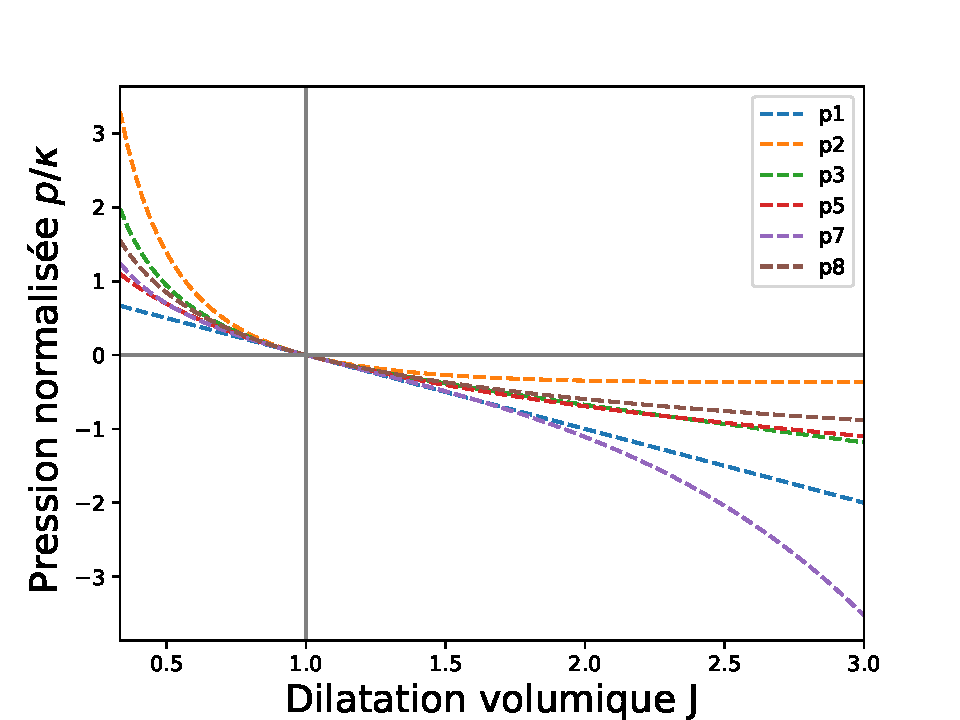
\includegraphics[width=0.7\textwidth]{fig/U_EOS}
\caption{Comparaison des pressions associées aux différentes énergies $U_{i}$}
\label{eq:p_Ui}
\end{figure}
\FloatBarrier
A ces lois ne disposant que d'un seul paramètre de compressibilité $\BulkModulus$, nous pouvons ajouter les deux lois suivantes comportant respectivement deux et trois paramètres:
\begin{table}
\centering \begin{tabular}{|c|l|}\hline
\widecellh{2.5}{1.5}{$U_{4}$} & $U_{4}(J)=\BulkModulus\theta^{-2}\pa{\theta\ln J +J^{-\theta} - 1}; \theta<-1$\\\hline
\widecellh{3}{2.5}{$U_{6}$} & $U_{6}(J)=\BulkModulus\pa{(1+\alpha)^{-1}J^{1+\alpha}+(\beta - 1+)^{-1}J^{1-\beta)}}(\alpha+\beta) - \dfrac{\BulkModulus}{(1+\alpha)(\beta-1)}$\\\hline
\end{tabular}
\label{tableau:energie_isotherme_hyperelast_complique}
\end{table}
\FloatBarrier
\paragraph{Lois d'état anisothermes associées}
Pour étendre ces lois au cas anisotherme, nous postulons que dans une expérience de dilatation libre, la dilatation volumique $\J_{libre}$ à pression nulle s'exprime en fonction de l'écart à une température de référence par:
$$\J_{libre} = 1 +\beta(T-T_{0}) \quad \beta:\text{coef de dilatation thermique à contrainte nulle}$$
Nous supposons de plus que la pression s'écrit:
$$p(T,\J)=p_{th}(T)+p_{vol}(\J)$$
Expression dans laquelle $p_{vol}(\J)$ désigne la pression donnée dans le \tableref{tableau:energie_isotherme_hyperelast}.
Nous prenons, pour exemple, la loi d'état $p_{8}$. La condition de pression nulle en dilatation libre nous donne:
$$p(T,J_{libre})=0 \implique p_{th}(T) =\dfrac{\BulkModulus}{2}\pa{\ln\pa{1+\beta(T-T_{0})} +1-\dfrac{1}{1+\beta(T-T_{0})}}$$
Dont on déduit la pression actuelle simplifiée ainsi que l'énergie dont dérive cette pression:
$$\begin{aligned}
p_{8}(T,J)&=-\dfrac{\BulkModulus}{2}\pa{\ln J-\dfrac{1}{J}-\ln\pa{1+\beta(T-T_{0})} +\dfrac{1}{1+\beta(T-T_{0})}}\\
U_{8}(T,J)&=\dfrac{\BulkModulus}{2}(J-1)\pa{\ln J-\ln\pa{1+\beta(T-T_{0})}-1+\dfrac{1}{1+\beta(T-T_{0})}}\\
\end{aligned}$$
Par le même raisonnement, nous en déduisons les pressions anisothermes $p_{i}(T,\J)$ généralisant celles du \tableref{tableau:energie_isotherme_hyperelast}:
\begin{table}
\centering \begin{tabular}{|l|}\hline
\widecellh{2.5}{1.5}{$p_{1}(\J,T)=-\BulkModulus(J-1-\beta(T-T_{0}))$}\\\hline
\widecellh{4.5}{2.5}{$p_{2}(\J,T)=-\BulkModulus\left(\dfrac{\ln \J}{J}-\dfrac{\ln\left(1+\beta(T-T_{0})\right)}{1+\beta(T-T_{0})}\right)$}\\\hline
\widecellh{4.5}{3.5}{$p_{3}(\J,T)=-\dfrac{\BulkModulus}{2}\left(\J-1 -\beta(T-T_{0})+\dfrac{\ln \J}{J}-\dfrac{\ln\left(1+\beta(T-T_{0})\right)}{1+\beta(T-T_{0})}\right)$}\\\hline
\widecellh{2.5}{1.5}{$p_{5}(\J,T)=-\BulkModulus\left(\ln\J-\ln\left(1+\beta(T-T_{0})\right)\right)$}\\\hline
\widecellh{4.5}{3.5}{$p_{7}(\J,T)=-\dfrac{\BulkModulus}{2}\left(\exp(J-1)-\exp(\beta(T-T_{0}))-\dfrac{1}{J}+\dfrac{1}{1+\beta(T-T_{0})}\right)$}\\\hline
\widecellh{4.5}{3.5}{$p_{8}(\J,T)=-\dfrac{\BulkModulus}{2}\left(\ln\J-\ln\left(1+\beta(T-T_{0})\right)-\dfrac{1}{J}+\dfrac{1}{1+\beta(T-T_{0})}\right)$}\\\hline
\end{tabular}
\caption{Energies volumiques et lois d'états anisothermes}
\label{tableau;energie_anisotherme_hyperelast}
\end{table}
\FloatBarrier
\subsection{Équation d'état Mie-Grunensien}
Deux lois d'états de Mie-Gruneïsen, respectivement référencées par \og
MG \fg{} et \og xMG \fg{} sont actuellement codées dans le code CHARON. La pression actuelle est paramétrée dans les deux cas par la masse volumique et l'énergie interne. Nous rappelons que la masse volumique actuelle et sa valeur de référence sont reliées par $\dfrac{\rho_{0}}{\rho}=\det\GT$.
\begin{Propo}{Loi d'état xMG} La loi d'état xMG reliant la pression à $T$ et $J$ s'écrit:
$$p(T,J)=\dfrac{\rho_{0}c_{0}^{2}\ppart{\mu}\left(1+\left(1-\Gamma_{0}/2\right)\mu-b/2\mu^{2}\right)}{1-(s_{1}-1)\mu-s_{2}\mu^{2}J-s_{3}\mu^{3}J^{2}}+\rho_{0}c_{0}^{2}\npart{\mu}+\dfrac{\rho_{0}}{J}\left(\Gamma_{0}+b\ppart{\mu}\right)e$$
expression dans laquelle nous avons introduit la variable réduite $\mu$ définie par:
$$\mu=\dfrac{\rho}{\rho_{0}}-1=\dfrac{1}{\det\GT}-1=\dfrac{1}{\J}-1$$
\end{Propo}
\subsubsection{Loi d'état MG}
\begin{equation}
p=P_{A}+\Gamma_{0}\rho e+C\mu+D\mu^{2}+S\mu^{3}=h(\rho,e)
\label{eq:PMG}
\end{equation}
Cette loi est parfois simplifiée en isotherme et sans pression initiale $P_{A}$. Dans ce cas, dans la limite des petites déformations on a $\mu \approx -\tr\DefoHPP$, et $C$ peut s'identifier à un module de compressibilité tangent.
Notons que cette équation n'est valable que si $\tilde{\rho}>1$. Dans le cas contraire, la loi s'écrit:
$$p=p_{A}+\rho_{0}\tilde{\rho}\left(H+(\Gamma_{0}-H)\left(\tilde{\rho}\right)^{n}\right)\left(e-e_{s}A\left[1-\exp\left(B(e)\frac{1}{\tilde{\rho}}\left(1-\frac{1}{\tilde{\rho}}\right)\right)\right]\right)$$
avec $B$ une fonction assurant la continuité de la dérivée avec le cas $\tilde{\rho}>1$ définie par:
$$B(e)=\max\left(0,\dfrac{C-e\rho_{0}(\Gamma_{0}-H)n}{\Gamma_{0}\rho_{0}e_{s}A}\right)$$
Nous pouvons réécrire ces deux lois en définitive en introduisant la partie positive aussi appelée crochet de MacKauley.
\begin{Propo}{Loi d'état MG} La loi d'état MG reliant la pression à $T$ et $J$ s'écrit:
$$\begin{aligned}
p =& \left\{P_{A}+\Gamma_{0}\rho e+C\left(\dfrac{\rho}{\rho_{0}}-1\right)+D\left(\dfrac{\rho}{\rho_{0}}-1\right)^{2}+S\left(\dfrac{\rho}{\rho_{0}}-1\right)^{3}\right\}\Heav(\tilde{\rho}-1)\\
&+\left\{P_{A}+\rho_{0}\tilde{\rho}\left(H+(\Gamma_{0}-H)\left(\tilde{\rho}\right)^{n}\right)\left(e-e_{s}A\left[1-\exp\left(B(e)\frac{1}{\tilde{\rho}}\left(1-\frac{1}{\tilde{\rho}}\right)\right)\right]\right)\right\}\Heav(1-\tilde{\rho})
\end{aligned}$$
\end{Propo}
\subsection{Loi d'état de Vinet}
La loi d'état de Vinet \cite{vinet1987temperature} postule la relation suivante entre la dilatation volumique $\J$, la température $T$ et la pression:
\begin{equation}
p_{\mathrm{Vinet}}(T,\J)=3K_{0}(T)\J^{-2/3}(1-\J^{1/3})e^{\frac{3}{2}(K_{1}(T)-1)(1-\J^{1/3})} \avec \left\lbrace
\begin{aligned}
K_{0}(T)&=K_{0}^{iso-T}+K_{0}^{T}T\\
K_{1}(T)&=K_{1}^{iso-T}+K_{1}^{T}T
\end{aligned}\right. 
\label{eq:eos_Vinet}
\end{equation}
La rigidité tangente (initiale) du modèle de Vinet est donnée par:
$$\begin{aligned}
\BulkModulus_{0} &= \dfrac{\partial p_{\mathrm{Vinet}}}{\partial \J}(\J=1, T=0)=\left[3K_{0}(T)\times \dfrac{1}{3}J^{-2/3}\J^{-2/3}e^{\frac{3}{2}(K_{1}(T)-1)(1-\J^{1/3})}+\underbrace{\dots}_{\text{termes nuls en }\J=1}\right](\J=1,T=0)\\
&=K_{0}(T)
\end{aligned}$$
\newcommand{\Gruneisen}{\Gamma}
\subsection{Loi d'état JWL}
L'équation d'état JWL utilisée pour la simulation de produits (et parfois de réactifs) d'explosif à forte puissance. La forme analytique dans une forme simplifiée, précisée par \cite{menikoff2015jwl} équation (16.b), est implémenté dans le code CHARON, et s'écrit comme suite:
$$p(V,T) = A \exp(-R_1 v) + B \exp(-R_2 v) +\dfrac{\Gruneisen }{V}C_{V}T$$
avec $v=\dfrac{V}{V_{0}}=\dfrac{\rho_{0}}{\rho}=\J$, $C_{V}$ en $\joule.\kelvin^{-1}$, $\dfrac{C_{V}}{V}=\rho \Cm$ où $\Cm$ en $\joule.\kelvin^{-1}\kilo\gram^{-1}$ désigne la capacité thermique massique.

Cette loi souffre d'un domaine d'utilisation restreint en dehors duquel des solutions fantaisistes peuvent apparaître (coefficient de compressibilité négatif par exemple) (voir à nouveau \cite{menikoff2015jwl} pour une discussion à ce sujet).
\begin{Defi}{Loi d'état JWL} Nous postulons la forme suivante pour la partie sphérique de la contrainte:
\begin{equation}
p_{\mathrm{JWL}}(T,\J)=Ae^{-R_{1}J}+Be^{-R_{2}J}+\Gruneisen  \rho \Cm T
\label{eq:loi_etat_JWL}
\end{equation}
\end{Defi}
Nous pouvons ainsi proposer une approximation de la célérité des ondes acoustiques en évaluant comme dans la \secref{Section:Exercices développeurs}:
$$\begin{aligned}
\dfrac{\partial p}{\partial \rho}&=\dfrac{\partial p}{\partial J}\dfrac{\partial J}{\partial \rho}=-\dfrac{J^{2}}{\rho_{0}}\left(-AR_{1}e^{-R_{1}J}-BR_{2}e^{-R_{2}J}\right)\\
c&=\sqrt{\dfrac{\partial p}{\partial \rho}(\rho=\rho_{0})}=\sqrt{\dfrac{AR_{1}e^{-R_{1}}+BR_{2}e^{-R_{2}}}{\rho_{0}}}
\end{aligned}$$
La loi d'état \eqref{eq:loi_etat_JWL} impose les paramètres suivants en entrée:
\begin{itemize}
\item $A$, en \pascal
\item $R_{1}$, sans dimension
\item $B$, rôle symétrique au coefficient $A$
\item Coefficient $R_{2}$, rôle symétrique au coefficient $R_{1}$.
\item $\Gruneisen$, paramètre de Gruneisen
\item $\Cm$, capacité thermique massique.
\item $\rho_{0}$, masse volumique initiale.
\end{itemize}
En linéarisant \eqref{eq:loi_etat_JWL} pour des déformations volumique $\J$ proches de l'unité, nous remarquons que:
$$\begin{aligned}
p_{\mathrm{JWL}}(T,\J)&=Ae^{-R_{1}}e^{-R_{1}\tr\DefoHPP}+Be^{-R_{2}}e^{-R_{2}\tr\DefoHPP}+\Gruneisen  \rho \Cm T\\
&\approx Ae^{-R_{1}}(1-R_{1}\tr\DefoHPP)+Be^{-R_{2}}(1-R_{2}\tr\DefoHPP)+\Gruneisen  \rho \Cm T\\
&\approx p_{0}(T)-\BulkModulus \tr\DefoHPP \avec \BulkModulus = AR_{1}e^{-R_{1}}+BR_{2}e^{-R_{2}}
\end{aligned}$$
Le groupement $AR_{1}e^{-R_{1}}+BR_{2}e^{-R_{2}}$ joue donc le rôle d'un module de compressibilité initial tangent et doit être choisit avec cohérence. Nous aurions pu également évaluer cette rigidité tangente en calculant $\dfrac{\partial p}{\partial \J}(\J=1)$
\begin{Rem}{Si $\J \gg 1$, les deux premiers termes de \eqref{eq:loi_etat_JWL} deviennent négligeable et la loi d'état se ramène à celle d'un gaz parfait mentionnée dans la prochaine partie. En effet, $\Cm T =\EIntMass$ et $\Gamma = \gamma - 1$.}\end{Rem}
\subsection{Loi d'état MACAW}
\paragraph{Partie froide}
Basé sur \cite{lozano2022robust}, nous appelons courbe froide de Macaw l'équation d'état (anisotherme) suivante:
\begin{equation}
P_{c}(\J)=A\J^{-B+1}\exp\left(\dfrac{2}{3}C\left(1-\J^{3/2}\right)\right)\left(C\J^{3/2}+B\right) - A(B+C)
\label{eq:P_isoT_MACAW}
\end{equation}
où $A$ (en \pascal), $B$ (sans dimension), $C$ (sans dimension) sont trois constantes positives (voir eq(7) de \cite{lozano2023analytic}).
\paragraph{Partie thermique} La partie thermique \cite{lozano2023analytic} nécessite de nouveaux coefficients: $\{\eta, V_{0}, \theta_{0}, a_{0}, m, n,\Gamma_{\infty},\Gamma_{0}\}$ dont l'interprétation sera donnée ultérieurement. Afin de simplifier l'écriture de équation d'état, nous introduisons les fonctions auxiliaires $\theta$ et $a$ suivantes:
\begin{equation}
\begin{aligned}
\theta(\J)&=\theta_{0}\J^{-\Gamma_{0}}\eta^{-\Gamma_{0}}\left(\J^{-m}\eta^{-m}+1\right)^{\frac{\Gamma_{\infty}-\Gamma_{0}}{m}}\\
a(\J)&=\dfrac{a_{0}}{1+\J^{-n}\eta^{-n}}
\end{aligned}
\label{eq:theta_J_a_J_MACAW}
\end{equation}
Dans le code CHARON, et contrairement au travail de \cite{lozano2022robust} qui considère que les fonctions ci-dessus dépendent du volume massique $V$, nous paramétrons $\theta$ et $a$ par la dilatation volumique $\J$. Nous rappelons que $\dfrac{\d\theta(V)}{\d V}=\dfrac{1}{V_{0}}\dfrac{\d\theta(\J)}{\d\J}$. Nous avons alors:
\begin{equation}
\begin{aligned}
\dfrac{\d\theta(V)}{\d V}=&\dfrac{1}{V_{0}}\left(-\dfrac{\Gamma_{0}}{\J}\theta(\J)+\dfrac{\Gamma_{\infty}-\Gamma_{0}}{m}\dfrac{1}{1+\J^{-m}\eta^{-m}}\eta^{-m}(-m)\J^{-m-1}\theta(\J)\right)\\
&=\dfrac{\theta(\J)}{V_{0}\J}\left(-\Gamma_{0}-\dfrac{\Gamma_{\infty}+\Gamma_{0}}{1+\J^{m}\eta^{m}}\right)\\
&=-\dfrac{\theta(\J)}{V_{0}\J}\dfrac{\Gamma_{\infty}+\Gamma_{0}\J^{m}\eta^{m}}{1+\J^{m}\eta^{m}}
\end{aligned}
\label{eq:deriv_theta_J_MACAW}
\end{equation}
Par ailleurs:
\begin{equation}
a'(V)=\dfrac{1}{V_{0}}\dfrac{a_{0}n\eta^{-n}\J^{-n-1}}{(1+\J^{-n}\eta^{-n})^{2}}=\dfrac{1}{V_{0}}\dfrac{a_{0}n\eta^{n}\J^{n}}{\J(1+J^{n}\eta^{n})^{2}}
\label{eq:deriv_aJ_MACAW}
\end{equation}
$\theta$, $a$ et leurs dérivées nous permettent alors de définir trois fonctions $q_{0}$, $q_{1}$, $q_{2}$:
$$\begin{aligned}
q_{0}&=\dfrac{1}{3}a'(V)-\dfrac{1}{\theta(\J)}\theta'(V)\\
q_{1}&=\dfrac{5\theta}{6}a'(V)-\dfrac{a}{6}\theta'(V)\\
q_{2}&=\dfrac{\theta^{2}}{2}a'(V)-\dfrac{a\theta}{2}\theta'(V)\\
\end{aligned}$$
qui sont homogènes à l'inverse d'un volume massique \ie à une densité (en $\kilo\gram.\metre^{-3}$).

Et d'écrire la partie thermique de l'équation d'état sous la forme:
\begin{equation}
P_{th}(T,V)=\dfrac{C_{v}^{\infty}}{(T+\theta)^{3}}\left(q_{0}T^{4}+q_{1}T^{3}+q_{2}T^{2}\right)
\label{eq:P_T_MACAW}
\end{equation}
où $C_{v}^{\infty}$ (en $\joule.\kelvin^{-1}\kilo\gram^{-1}$) désigne la capacité thermique massique à volume constant. Pour plus de clarté, nous la noterons dans la suite $C_{v}^{\infty} = \Cm^{\infty}$.\\

L'expression de la pression totale $P$ s'écrit ensuite en superposant les contributions \eqref{eq:P_isoT_MACAW}, \eqref{eq:P_T_MACAW}.
\paragraph{Célérité}
Comme habituellement une estimation de la célérité des ondes est obtenue en calculant 
$$c = \dfrac{\partial P}{\partial \rho}(\rho = \rho_{0})=-\dfrac{\J^{2}}{\rho_{0}}\dfrac{\partial P}{\partial \J}(J=1)$$
Cette expression étant particulièrement lourde, nous la calculons ici avec Sympy.

Une estimation plus simple de la célérité peut être obtenue en supposant la correction de la température négligeable. Le module de compressibilité du modèle de MACAW est donné par (voir eq (18) de \cite{lozano2022robust}) et peut être utilisé pour donné l'estimation suivante de la vitesse des ondes:
$$c\approx \sqrt{\dfrac{K_{0}}{\rho_{0}}} \avec K_{0}=A\left(B-\dfrac{1}{2}C+(B+C)^{2}\right)$$
\paragraph{Capacité thermique} La capacité thermique massique dans ce cas est donnée par:
$$\Cm(\J,\tau)=\Cm^{\infty}\dfrac{\tau^{4}+4\tau^{3}+a(\J)\tau}{(\tau+1)^{4}} \avec \tau = T/\theta(\J)$$
\paragraph{Synthèse} Nous rappelons ici l'ensemble des paramètres et des fonctions nécessaire à la définition de la loi d'état de Macaw. L'expression de la pression $P$ est la superposition de deux termes:
$$\begin{aligned}
P_{c}(\J)&=A\J^{-B+1}\exp\left(\dfrac{2}{3}C\left(1-\J^{3/2}\right)\right)\left(C\J^{3/2}+B\right)-A(B+C)\\
P_{th}(T,\J)&=\dfrac{\rho_{0}\Cm^{\infty}}{(T+\theta)^{3}}\left(\tilde{q}_{0}T^{4}+\tilde{q}_{1}T^{3}+\tilde{q}_{2}T^{2}\right)
\end{aligned}$$
avec les trois fonction $\tilde{q}_{i}$ sans dimension:
$$\begin{aligned}
\tilde{q}_{0}&=\dfrac{1}{3}a'(\J)-\dfrac{1}{\theta(\J)}\theta'(\J)\\
\tilde{q}_{1}&=\dfrac{5\theta}{6}a'(\J)-\dfrac{a}{6}\theta'(\J)\\
\tilde{q}_{2}&=\dfrac{\theta^{2}}{2}a'(\J)-\dfrac{a\theta}{2}\theta'(\J)\\
\end{aligned}$$
lesquelles font intervenir:
$$\begin{aligned}
\theta(\J)&=\theta_{0}\J^{-\Gamma_{0}}\eta^{-\Gamma_{0}}\left(\J^{-m}\eta^{-m}+1\right)^{\frac{\Gamma_{\infty}-\Gamma_{0}}{m}}\\
a(\J)&=\dfrac{a_{0}}{1+\J^{-n}\eta^{-n}}\\
\theta'(\J)&=-\dfrac{\theta(\J)}{\J}\dfrac{\Gamma_{\infty}+\Gamma_{0}\J^{m}\eta^{m}}{1+\J^{m}\eta^{m}}\\
a'(\J)&=\dfrac{a_{0}n\eta^{n}\J^{n}}{\J(1+J^{n}\eta^{n})^{2}}
\end{aligned}$$
Ces lois nécessitent la donnée de 12 coefficients :
\begin{center}
\begin{tabular}{ll|ll|ll|ll}
$A$ & Pascal & $\eta$ & Sans dimension ($=\frac{V_{0}}{V_{\infty}}$) & $m$ & Sans dimension & $\Gamma_{0}$ & Sans dimension\\
&&&&&&&\\
$B$ & Sans dimension & $a_{0}$ & Sans dimension & $n$ & Sans dimension & $\Cm^{\infty}$ & $\joule.\kelvin^{-1}\kilo\gram^{-1}$ ($=C_{v}^{\infty}$)\\
&&&&&&&\\
$C$ & Sans dimension & $\theta_{0}$ & Kelvin & $\Gamma_{\infty}$ & Sans dimension & $\rho_{0}$ & $\kilo\gram.\metre^{-3}$ ($=\frac{1}{V_{0}}$)\\
\end{tabular}
\end{center}
La capacité thermique massique est alors donné par:
$$\Cm(T,\J)=\Cm^{\infty}\dfrac{\tau^{4}+4\tau^{3}+a(\J)\tau}{(\tau+1)^{4}} \avec \tau = T/\theta(\J)$$
\begin{Rem}{La calibration de paramètres sur des expériences de dynamique moléculaires pour reproduire l'équation d'état peut parfois donner une estimation incorrecte de la capacité thermique $\Cm^{\infty}$ c'est pourquoi il est parfois nécessaire d'introduire un nouveau paramètre matériau $\Cm$ (bien qu'incohérent) qui intervient dans l'équation de la chaleur.}\end{Rem}
\subsection{Loi de comportement gaz parfait} 
\begin{Defi}{Loi d'état du gaz parfait} Dans ce modèle, la pression est donnée par la loi des gaz parfaits:
\begin{equation}
p_{\mathrm{GP}}=\dfrac{\rho R T}{M}
\label{eq:loi_pression_GP}
\end{equation}
\end{Defi}
La contrainte tridimensionnelle $\SC = -p\TU$ est bien une fonction seule de la température et de la déformation. \eqref{eq:loi_pression_GP} décrit bien une loi élastique au sens du point \ref{point:3_defi_elast} de la \defiref{Defi:Solide_elastique}.
Si l'on introduit le coefficient de Laplace $\gamma$ , \eqref{eq:loi_pression_GP} peut se réécrire:
$$p_{\mathrm{GP}}(T,\J) = (\gamma - 1)\rho \Cm T\avec \rho = \dfrac{\rho_{0}}{\J}$$
En effet on a les relations :
$$\begin{aligned}
C_{p}-C_{v} &= \dfrac{n R \gamma}{\gamma-1} - \dfrac{n R}{\gamma-1} = \dfrac{m R}{M}\\
&=(\gamma - 1)C_{v}
\end{aligned}$$
Autrement dit en introduisant $\Cm$ la capacité thermique massique à volume constant $\Cm = C_{v}/m$ :
$$\dfrac{R}{M} = (\gamma - 1)\Cm \implique p_{\mathrm{GP}} = \rho(\gamma - 1)\Cm T$$
Il est également possible de ré-exprimer cette loi avec le paramètre de Gruneisen $\Gamma$ qui dans le cas d'un gaz parfait vaut:
$$\Gruneisen = \gamma - 1$$
mais aussi en introduisant l'énergie interne massique que l'on prend ici égale à $\EIntMass = \Cm T$.

La célérité du son, notée $c$, est définie thermodynamiquement comme la racine carrée de la dérivée partielle de la pression par rapport à la masse volumique à entropie constante :
\begin{equation}
c^2 = \left(\frac{\partial p}{\partial \rho}\right)_s
\end{equation}
Cette définition découle de l'analyse des petites perturbations dans un fluide compressible, où les ondes acoustiques se propagent de manière isentropique. Or, pour un processus isentropique dans un gaz parfait, on a la relation suivante :
$$\frac{p}{\rho^\gamma} = \text{constante} \equivalent p = C\rho^\gamma$$
où $C$ est une constante pour un processus isentropique donné. À partir de la définition thermodynamique et de la propriété isentropique, calculons la célérité du son :
$$\begin{aligned}
c^2 &= \left(\frac{\partial p}{\partial \rho}\right)_s = \frac{\partial}{\partial \rho}(C\rho^\gamma)=\gamma C \rho^{\gamma - 1}\\
&= \gamma \frac{p}{\rho^\gamma}\rho^{\gamma-1} \quad \text{car }C = \dfrac{p}{\rho^{\gamma}}\\
&= \gamma \frac{p}{\rho}\\
&= \gamma (\gamma - 1) \EIntMass
\end{aligned}$$
\section{Juxtaposition ad-hoc de la loi déviatorique}\label{Section:Juxtaposition ad-hoc de la loi déviatorique}
Le terme \og hydrodynamique \fg{}, associé à un problème de mécanique du solide, précise que les sollicitations déformant le matériau à l'étude, induisent un champ de pression qui domine, de plusieurs ordres de grandeur, le déviateur des contraintes.\\

La loi d'état, objet d'étude de la précédente \secref{Section:Loi d'état} est donc de loin la partie la plus critique de la relation de comportement. Toutefois, les métaux soumis aux ondes de chocs ne se comportent pas complètement comme des fluides et exhibent toujours des comportements plastiques. Ces comportements ne sont envisageables que si la l'équation d'état est complétée par une loi déviatorique. Cette complétion est \emph{ad-hoc} en postulant, tantôt une loi déviatorique HPP, tantôt une loi corrigée pour prendre en compte les effets de compressibilité sur le module de cisaillement. Dans le code CHARON, trois lois déviatoriques sont actuellement implémentées et correspondent à celle présentées dans le \chapref{Chapitre:Elasticité}. La loi de comportement globale s'écrit donc:
$$\SC = -\underbrace{p(T,\rho)}_{EOS}\TU+\devia$$
\subsection{Loi déviatorique élastique linéaire}
\begin{Propo}{Loi déviatorique élastique linéaire isotrope} Nous postulons le déviateur des contraintes suivant \cite{forest2015mecanique}:
\begin{equation}
\devia =2\mu\dev\DefoHPP
\label{eq:loi_deviateur_HPP_analytique}
\end{equation}
\end{Propo}
\subsection{Loi déviatorique Néo-Hookéenne}
La loi déviatorique Néo-Hookéenne correspond à un développement au premier ordre de l'énergie libre de Helmholtz par rapport au premier invariant du tenseur de déformation de Cauchy-Green gauche isochore \cite{bouteiller2023complete}:
\begin{equation}
\eHelmMass = U(J) + \dfrac{\mu}{2}\left(\BBarI -3\right)
\label{eq:postulat_eHelm_NH}
\end{equation}
\begin{Propo}{Comportement déviatorique Néo-Hookéen} Le comportement déviatorique résultant de l'énergie \eqref{eq:postulat_eHelm_NH} est:
\begin{equation}
\devia = \frac{\mu}{\J^{\frac{5}{3}}}\dev\CGG
\label{eq:loi_deviateur_NH_analytique}
\end{equation}
\end{Propo}
Pour des transformations infinitésimales, on a au premier ordre:
$$\CGG \approx \TenUnit + 2\DefoHPP \implique \dev\CGG \approx 2\dev\DefoHPP$$
De sorte que le coefficient de cisaillement $\mu$ intervenant dans \eqref{eq:loi_deviateur_NH_analytique} a la même interprétation que celui dans \eqref{eq:loi_deviateur_HPP_analytique}.
\subsection{Loi déviatorique de Mooney-Rivlin}
La loi déviatorique de Mooney-Rivlin correspond à un développement au premier ordre de l'énergie libre de Helmholtz par rapport aux deux invariants du tenseur de déformation de Cauchy-Green gauche isochore:
\begin{equation}
\eHelmMass = U(J) + \dfrac{C_{10}}{2}\left(\BBarI -3\right)+ \dfrac{C_{01}}{2}\left(\BBarII -3\right)
\label{eq:postulat_eHelm_NH}
\end{equation}
\begin{Propo}{Comportement déviatorique de Mooney-Rivlin} Le comportement déviatorique résultant de l'énergie \eqref{eq:postulat_eHelm_NH} est:
$$\devia=\dfrac{\mu}{\J^{\frac{5}{3}}}\dev\CGG-\dfrac{C_{01}}{\J^\frac{7}{3}}\dev\left(\CGG^{2}-\tr(\CGG)\CGG\right)$$
\end{Propo}
Cette loi est une correction d'ordre supérieure au modèle Néo-Hookéen généralisé précédemment présenté. 

Si l'on suppose à nouveau que la transformation infinitésimale:
$$\CGG^{2}-\tr(\CGG)\CGG\approx (\TenUnit+4\DefoHPP) - (3+2\tr\DefoHPP)(\TenUnit+2\DefoHPP) \implique \dev\left(\CGG^{2}-\tr(\CGG)\CGG\right)\approx -2\dev\DefoHPP$$
De sorte que l'on doit assurer $C_{10}+C_{01}=\mu$ afin d'être cohérent avec la modélisation en petites perturbations.

%\newcommand{\TenVMAnis}{\PP}
%\newcommand{\DeltaSC}{\ten{\Delta}\SC}
\newcommand{\DeltaDefoHPP}{\ten{\Delta}\DefoHPP}
\newcommand{\DeltaEpsP}{\DeltaDefoHPP^{p}}
%\newcommand{\ConvElas}{C}
%\newcommand{\TenNormale}{\ten{N}}
%\newcommand{\CentreConv}{\ten{X}}
%\newcommand{\HatSigRel}{\hat{\ten{\psi}}_{Rel}}
%\newcommand{\ChalMassUn}{q_{exp}^{m\, (1)}}
\chapter{Plasticité}\label{Chapitre:Plasticité}
\section*{\emph{Introduction}}
Soumise à des sollicitations plus importantes, une vaste gamme de métaux exhibe un comportement anélastique caractéristique appelé \emph{plasticité}. Ce comportement traduit macroscopiquement la réorganisation et le mouvement de dislocations à l'échelle du réseau cristallin.\\

Il est possible d'envisager la plasticité dans deux régimes. Celui des petites perturbations et le cadre des transformations finies. Historiquement au CEA, la plasticité a été introduite comme une correction aux lois d'états utilisées et par conséquent restreinte au cadre des petites perturbations malgré le fait que les expériences envisagées s'en écartent résolument...
\begin{itemize}[label=$\star$]
\item  La \secref{Section:Introduction de la plasticité HPP} présente les lois de plasticités dans l'hypothèse des petites perturbations actuellement implémentées dans le code CHARON.
\end{itemize}
\section{Plasticité dans l'hypothèse des petites perturbations}\label{Section:Introduction de la plasticité HPP}
\begin{Postulat}{Plasticité isotrope dans l'hypothèse des petites perturbations} La contrainte tridimensionnelle est \emph{postulée de la forme}:
$$\SC=-p(T,\J)\TenUnit+2\mu(\dev\Eps-\EpsP)$$
\end{Postulat}
La plasticité est matérialisée par un tenseur de déformation plastique $\EpsP$, lequel abat la contrainte tridimensionnelle de Cauchy. Le tenseur de déformation plastique évolue lorsque la contrainte locale dépasse un certain seuil caractérisé par une fonction $\FChargeConvexe$ appelée \emph{fonction de charge} qui délimite une zone convexe dans le domaine des contraintes. Si la contrainte actuelle demeure à l'intérieur de ce convexe, la plasticité n'évolue pas. Par isotropie, la fonction $\FChargeConvexe$ ne dépend habituellement que des invariants du tenseur des contraintes: $\tr(\SC)$, $J_{2}(\devia) = \dfrac{1}{2}\devia:\devia$, $J_{3}(\devia) = \dfrac{1}{3}\tr\devia^{3}$.
\paragraph{L'écrouissage} Le domaine de réversibilité peut varier au cours du temps ou plus exactement au fur et à mesure que la déformation plastique évolue. Lorsque le domaine est fixe, on parle de \emph{plasticité parfaite}, alors que quand il varie, on parle de \emph{plasticité avec écrouissage}. Cet écrouissage s'interprète comme la difficulté qu'ont les dislocations de se développer du fait de la présence d'amas de dislocations précédemment créées.
\section{Elasto-plasticité en transformations finies}\label{Section:Elasto-plasticité en transformations finies}
\newcommand{\argmin}{\mathrm{arg}\,\min}
\newcommand{\PPot}{\Phi}
\chapter{Endommagement}\label{Chapitre:Endommagement}
\section*{\emph{Introduction}}
Pour finir, lorsque le matériau est soumis à des conditions extrêmes, la création et la coalescence de trous conduisent à une rupture macroscopique du matériau. Pour modéliser ce phénomène, une variable d'endommagement $d$ scalaire, prenant ses valeurs entre 0 et 1 dégrade continûment la rigidité du matériau. La contrainte actuelle est donc pondérée de la manière suivante:
$$\SC = g(d)\SC(\Dep,T)$$
où $g$ désigne une fonction décroissante vérifiant $g(0)=1$ (lorsque le matériau n'est pas endommagé la contrainte égalise sa valeur de référence), et $g(1)=0$ (lorsque le matériau est complètement endommagé la contrainte est nulle). Un modèle simple consiste par exemple à prendre  $g(d)=1-d$.
Nous envisageons ici le modèle de Johnson comme un cas particulier de l'endommagement dans lequel la variable $d$ correspond à la porosité du matériau. L'objectif des sections à suivre et de préciser comment la variable d'endommagement est calculée.
\begin{itemize}
\item La première \secref{Section:Ajout de l'endommagement fragile} présente de manière succincte la prédiction de l'endommagement par la méthode de \og champ de phase \fg{}, historiquement développé pour la prédiction de la rupture fragile.
\item Une deuxième \secref{Section:Modèle cohésif} aborde la formulation cohésive de la rupture au travers d'éléments d'interface.
%\item Une troisième \secref{Section:Modèle de Johnson} présente le modèle de Johnson actuellement massivement utilisé. Il s'agit d'un modèle pilotant la croissante de la porosité d'un matériau soumis à une onde de choc. 
\end{itemize}
\section{Formulation variationnelle de la rupture fragile}\label{Section:Ajout de l'endommagement fragile}
Un premier modèle d'endommagement fragile a été implémenté sur le code CHARON. Une variable d'endommagement, définie sur l'ensemble du domaine $\Configuration_{t}$, traduit l'abattement des propriétés mécaniques du matériaux consécutif à une sollicitation excessive. La variable dégrade les propriétés mécaniques de manière isotrope:

L'évolution de la variable $d$ résulte d'une équation non locale, résolue avec le solveur TAO. Ce modèle s'inscrit dans le cadre de l'endommagement par champ de phase.
\subsection{Formulation variationnelle incrémentale}
La solution $(\Dep_{k+1},d_{k+1})$ au $k+1^{\text{ème}}$ pas de chargement est obtenue en minimisant la fonctionnelle énergie totale $\Etot_{k}$:
\begin{equation}
(\Dep_{k+1},d_{k+1}) = \argmin_{\Dep,d} \Etot_{k}(\Dep,d)
\label{eq:Minimisation_intra}
\end{equation}
où $\Etot_{k}$, sur ce pas de chargement, est la somme de l'énergie potentielle et d'une contribution du pseudo-potentiel de dissipation donnée par:
\begin{align}
\Etot_{k}(\Dep,d) &= \EPot(\Dep,d)+\mathcal{D}_{k}(d)\\
\EPot(\Dep,d) &=\int_{\Omega} \eHelm(\Dep,d)\dvt-\Wext(\Dep)\\
\mathcal{D}_{k}(d) &= \int_{\Omega}\varphi(d)\dvt
\avec \varphi(d)=\dfrac{\Gc}{\ell c_{w}}\left(w(d)+\ell^{2}\vec{\nabla d}\cdot\vec{\nabla d}\right)
\end{align}
$\Wext$ désigne le travail des forces extérieures, nous obtenons alors:
\begin{equation}
(\Dep_{k+1},d_{k+1})= \argmin_{\Dep,d \geq d_{k}} \Etot_{k}(\Dep,d) \avec 
\label{eq:incremental-energy-minimization}
\end{equation}
où la condition d'irréversibilité $\dot{d}\geq 0$ a été remplacée par la condition incrémentale $\d \geq d_{k}$. Le problème se résume alors à rechercher, de manière incrémentale, le minimum de la fonctionnelle énergie suivante:
\begin{equation}
\Etot(\Dep,d)=\int_{\Omega}\eHelm(\Dep,d)+\varphi(d,\vec{\nabla d}) \dvt -\Wext(\Dep)
\label{eq:fonctionnelle_energie_intra}
\end{equation}
Nous utilisons un algorithme de minimisation alternée:
\begin{itemize}[label=-]
\item La stationnarité par rapport à $\Dep$ nous donne un problème d'élasticité à $\d$ fixé.
\item La stationnarité par rapport à $\d$ se traduit par la minimisation sous contrainte d'inégalité:
\begin{equation}
d_{k+1}= \argmin_{\d \geq d_{k}} \Etot_{k}(\Dep,d)
\label{eq:minimisation_intralam_d}
\end{equation}
En pratique, l'évolution est assurée ($\dot{d}>0$) si la solution $d^{*}$ de \eqref{eq:evol_generale_intra}
\begin{equation}
-\dfrac{\partial \eHelm}{\partial d}(d^{*})=\dfrac{G_{c}}{\ell c_{w}}\left(w'(d^{*})-\ell^{2}\Delta d^{*}\right)
\label{eq:evol_generale_intra}
\end{equation}
est telle que $d^{*}>d_{k}$ sinon $d_{k+1}=d_{k}$.
\end{itemize}
\subsection{Expression de l'énergie libre de Helmolhtz}
Pour les modèles HPP et Néo-Hookéen, nous pouvons écrire les énergies libre de helmokhtz suivante:
$$\psi_{HPP}=\dfrac{\lambda}{2}(\tr\DefoHPP)^{2}+\mu\tr\left(\DefoHPP^{2}\right)$$
\section{Modèle phase-field de Miehe}
Miehe (METTRE REF) propose plutôt que d'imposer par un solveur d'optimisation sous contrainte. la formulation variationnelle suivante:
$$-g'(d^{*})\mathcal{H}^{+}=\dfrac{G_{c}}{\ell c_{w}}\left(w'(d^{*})-\ell^{2}\Delta d^{*}\right)$$
où $\Hh^{+}$ désigne une variable d'histoire définie comme suit:
$$\Hh^{+}=\max_{\tau\in[0,t]}\psi^{+}(\Dep)$$
Cette fois il s'agit d'un problème variationnelle linéaire en $d$ qui peut se réécrire en sélectionnant par exemple un modèle AT2 $g(d)=(1-d^{2})$, $w(d)=d^{2}$:
$$\int_{\Dmt}\left(\dfrac{\Gc}{2\ell}+\Hh^{+}\right)d\hat{d}+\dfrac{\Gc\ell}{2}\nabla d\cdot\nabla\hat{d}\dvt = \int_{\Dmt}\Hh^{+}\hat{d}\dvt$$
\section{Modèle cohésif}\label{Section:Modèle cohésif}
Un modèle de zone cohésif est disponible dans Charon. Les éléments finis retenus pour l'interpolation du champ de déplacement ne sont plus du type \emph{Continous Galerkin} mais de type \emph{Galerkin discontinu}. Une relation supplémentaire est alors nécessaire pour rattacher les différents éléments entre eux. Nous postulons qu'il existe une force cohésive supplémentaire, agissante entre les éléments:
$$\vec{T}(\jump{\Dep})=\dfrac{\Gc}{\delta_{0}^{2}}e^{-\frac{u_{eff}}{\delta_{0}}}\jump{\Dep}$$
$u_{eff}$ désigne un saut de déplacement effectif donné par exemple par:
$$u_{eff}=\sqrt{(\jump{\Dep}\cdot\vec{n})^{2}+\beta^{2}\left(\jump{\Dep}-\jump{\Dep}\cdot\vec{n}\vec{n}\right)^{2}}$$
La formulation variationnelle du problème est donc augmenté du travail de cette force de traction, agissant uniquement sur les frontières des éléments intérieures au domaine:
$$\Ww(\vec{T})=\int_{\partial\Omega_{int}}\vec{T}(\jump{\Dep})\cdot\jump{\DepVirt}\ds$$

\section{Modèle de Johnson}
\subsection{Position du problème}
\begin{Not}{Rayon du pore, de la boule et porosité} Nous notons $a(t)$ le rayon actuel de la cavité sphérique, $b(t)$ le rayon de la boule creuse englobant cette cavité sphérique (voir Figure \ref{pore_unique}). $\displaystyle f(t)=\dfrac{a(t)^3}{b(t)^3}$ désigne la porosité associée, sa valeur initiale est notée $f_0$.
 \end{Not}
\begin{Hypothese}{ de travail}Pour cette section, nous réalisons les hypothèses suivantes
\begin{enumerate}
\item Nous négligeons le comportement élastique du matériau
\item Nous supposons que le problème est à symétrie sphérique.
\item Les conditions aux limites en efforts sont les suivantes: la pression est nulle au sein de la cavité $p(a(t))=0$. Sur la surface extérieure de la coquille, $r=b(t)$, nous imposons la contrainte $\sigma_{rr}(b(t)) =p_e$.
\item\label{hyp4:incompressible} L'écoulement plastique est considéré incompressible
\item Nous négligeons l'influence des forces de volume.
\end{enumerate}
\end{Hypothese}
\begin{figure}[h!]
%\centering    \includegraphics[width=0.3\textwidth]{doc/pore_solitaire.png}
\captionof{figure}{Sphère creuse de rayon $b$ contenant un pore en croissance de rayon $a$.}
\label{pore_unique}
\end{figure}
\subsubsection{Aspects cinématiques}
L'écoulement plastique étant supposé incompressible (\ref{hyp4:incompressible}), les volumes de matière sont donc conservés tout au long de l'évolution.
 $$b^3(t)-a^3(t) = (1-f_0)\,b^3(0)$$
On définit, comme proposé dans \cite{Duplay_RI2004}, une fonction $\omega$ mesurant la différence de volume entre la cavité sphérique dans la configuration actuelle et initiale. Cette fonction mesure donc le \og volume additionnel de vide \fg{}.
\begin{equation}
\omega(t):=a^3(t)-a^3(0)=a^3(t)-f_0\,b^3(0)
\label{eq:defi_fonction_omega}
\end{equation}
Si nous écrivons la conservation du volume entre un point situé en $r(t)=a(t)$ et $r(t)$, la condition d’incompressibilité entre les instants initial et courant s'écrit:
$$r^{3}(t)-r^{3}_{0}=a^{3}(t)-a^{3}(0)$$
Autrement dit, si nous définissons $\tilde{\omega}:t\mapsto r^{3}(t)-r^{3}(0)$, alors $\forall t$, $\tilde{\omega}(t)=\omega(t)$.\\

L'hypothèse d'axi-symétrie indique que la vitesse et purement radiale $\vec{v}=v_{r}\er=\dot{r}(t)\er$. Elle peut s'obtenir en dérivant $\omega(t)=r^3(t)-r_0^3$ par rapport au temps:
\begin{equation}
\dot{r}(t)=\dfrac{\dot{\omega}(t)}{3\,r^2(t)}
\label{eq:rel_dot_r_omega}
\end{equation}
Le tenseur taux de déformation $\TD$ est donné par : $\TD=\dfrac{1}{2}\pa{\ten{\textmd{grad}}(\underline{v})+\ten{\textmd{grad}}^\top(\underline{v})}$
$$\TD= \begin{pmatrix}
\dfrac{v_r}{r}  & 0 & 0 \\
0 & \dfrac{v_r}{r}  & 0 \\
0 & 0 & \dfrac{v_r}{r} 
\end{pmatrix} = \begin{pmatrix}
\dfrac{\dot{r}}{r}  & 0 & 0 \\
0 & \dfrac{\dot{r}}{r}  & 0 \\
0 & 0 & \dfrac{\dot{r}}{r} 
\end{pmatrix} = \begin{pmatrix}
-\dfrac{2\,\dot{\omega}(t)}{3\,r^3} & 0 & 0 \\
0 & \dfrac{\dot{\omega}(t)}{3\,r^3}  & 0 \\
0 & 0 & \dfrac{\dot{\omega}(t)}{3\,r^3} 
\end{pmatrix}$$
Pour plus de concision, nous pouvons introduire un \og taux de déformation équivalent \fg{}:
\begin{equation}
d_{eq}:=\sqrt{\dfrac{2}{3}\,\TD:\TD}=\dfrac{2}{3}\dfrac{\dot{\omega}(t)}{r^3}
\label{eq:defi_taux_defo_equiv}
\end{equation}
\subsubsection{Équations d'équilibre}
Les symétries du problème permettent d'écrire le tenseur des contraintes de Cauchy: 
$$\ten{\sigma}= 
\begin{pmatrix}
\sigma_r  & 0 & 0 \\
0 & \sigma_\theta  & 0 \\
0 & 0 & \sigma_\theta 
\end{pmatrix} \implique \ten{s}= \begin{pmatrix}
\dfrac{2}{3}\left(\sigma_r-\sigma_\theta\right)  & 0 & 0 \\
0 & -\dfrac{1}{3}\left(\sigma_r-\sigma_\theta\right)  & 0 \\
0 & 0 & -\dfrac{1}{3}\left(\sigma_r-\sigma_\theta\right)
\end{pmatrix}$$
Dans la configuration déformée, la conservation de la quantité de mouvement s'écrit en négligeant les forces de volume:
\begin{align}\nonumber
\rho\,\dfrac{\underline{v}}{t} &= \vdiv_E\,\ten{\sigma}\\\nonumber
\implique \rho\,\ddot{r} &= (\vdiv_E\,\ten{\sigma})\cdot \er \quad \text{projection sur $\er$}\\\label{eq:equilibre_dyna}
\implique \rho\,\ddot{r} &=\dfrac{\sigma_r}{r}+ 2\dfrac{\sigma_r-\sigma_{\theta}}{r}
\end{align}
\subsection{Modèle de Johnson quasi-statique}
\begin{Hypothese}{Modèle quasi-statique} Nous choisissons pour la construction du modèle de Johnson quasi-statique de négliger le terme inertiel dans l'équation de la dynamique \eqref{eq:equilibre_dyna}.
\end{Hypothese}
Sous cette hypothèse, l'équation \eqref{eq:equilibre_dyna} se réduit à:
\begin{equation}
\dfrac{\sigma_r}{r} = 2 \,\dfrac{\sigma_\theta-\sigma_r}{r}
\label{eq:equillibre_statique}
\end{equation}
\begin{Hypothese}{Milieu complètement plastifié} Nous supposons de plus que le milieu est complètement plastifié et obéit à un critère de plasticité de Von-Mises:
\begin{equation}
\sigma_{eq} = \sqrt{\dfrac{3}{2}\ten{s}:\ten{s}}=|\sigma_r-\sigma_\theta| = \sigma_Y
\label{eq:critère_VM}
\end{equation}
avec une loi de comportement rigide visco-plastique parfait:
\begin{equation}
\sigma_Y = \sigma_0 +\eta \,\dot{\epsilon}_p
\label{eq:limite_elastique_visco_plast}
\end{equation}
où $\sigma_{Y}$ désigne classiquement la limite élastique du matériau. $\sigma_{0}$ désigne une limite élastique initiale, $\eta$ un coefficient de viscosité plastique et $\dot{\epsilon}_p$ le taux de déformation plastique défini par : 
 $$\dot{\epsilon}_p:=d_{eq} \quad d_{eq} \text{ donné par \eqref{eq:defi_taux_defo_equiv}}$$
\end{Hypothese}
La limite élastique $\sigma_{Y}$ \eqref{eq:limite_elastique_visco_plast} peut se réécrire en utilisant \eqref{eq:defi_taux_defo_equiv}:
\begin{equation}
\sigma_Y = \sigY + 2\,\eta\,\dfrac{\dot{\omega}(t)}{r^3}
\label{eq:nouvelle_expression_sigma_yield}
\end{equation}
En intégrant l'équation d'équilibre statique \eqref{eq:equillibre_statique} entre le rayon du pore $a(t)$ et le rayon extérieur $b(t)$, nous obtenons alors:
\begin{align}\nonumber
\Int{a(t)}{b(t)} \dfrac{\sigma_r}{r} \dr & = 2 \, \Int{a(t)}{b(t)}\dfrac{\sigma_\theta-\sigma_r}{r} \dr\\ &= 2\Int{a(t)}{b(t)}\pa{\dfrac{\sigma_0}{r}+   2\, \eta \,\dfrac{\dot{\omega}(t)}{r^4} }\, \dr \quad \eqref{eq:critère_VM} \et \eqref{eq:nouvelle_expression_sigma_yield}\\\nonumber
-p_e(t) & = 2 \,\sigma_0 \,\ln{\dfrac{b(t)}{a(t)}} +\dfrac{4}{3}\,\eta\,\dot{\omega}(t)\pa{\dfrac{1}{a(t)^3}-\dfrac{1}{b(t)^3}}\\\label{eq:porosite_avant_simpli}
-p_e(t) & = 2 \,\sigma_0 \,\ln{\dfrac{b(t)}{a(t)}} +\dfrac{4}{3}\,\dfrac{\eta\,\dot{\omega}(t)}{a^{3}(t)}\pa{1-f}
\end{align}
Or en dérivant temporellement la relation d'incompressibilité, nous obtenons:
$$b^{2}\dot{b}-a^{2}\dot{a}=0$$
Par ailleurs en dérivant toujours par rapport au temps la définition de la porosité, nous obtenons successivement:
$$\dot{f}=3\dfrac{a^{2}\dot{a}b^{3}-b^{2}\dot{b}a^{3}}{b^{6}}=3\left(\dfrac{\dot{a}f}{a}-\dfrac{a^{5}\dot{a}}{b^{6}}\right)=3\dfrac{\dot{a}}{a}f(1-f)$$
Pour finir, nous pouvons ré-exprimer la dérivée $\dot{f}$ à l'aide de la fonction $\omega$ définie à l'équation \eqref{eq:defi_fonction_omega}:
$$\dot{\omega}=3a^{2}\dot{a} \implique \dot{f}=\dfrac{\dot{\omega}}{a^{3}}f(1-f)$$
En remplaçant dans l'équation \eqref{eq:porosite_avant_simpli}, nous en déduisons alors:
$$-p_e(t)  = -\dfrac{2}{3} \,\sigma_0 \,\ln{f} +\dfrac{4}{3}\,\eta\,\dfrac{\dot{f}}{f}$$
Puis l'équation pilote de la porosité, également appelée équation de \og Johnson statique \fg{}:
\begin{equation}
\boxed{\dot{f} = -\dfrac{3}{4\,\eta}f\pa{p_e(t)-\dfrac{2}{3}\sigma_0\ln{f}}}
\label{eq:johnson_statique}
\end{equation}
Pour résoudre cette équation, seule la connaissance de $f(t=0)=f_0$ est nécessaire. Dans le code CHARON, les paramètres d'entrées du modèle de Johnson quasi-statique sont $\eta$ et $\sigma_{0}$ intervenant dans \eqref{eq:johnson_statique}. 
\subsection{Modèle de Johnson dynamique}
Le modèle de Johnson dynamique se distingue du cas précédent par la prise en compte du terme d’accélération dans l'équation de conservation de la quantité de mouvement \eqref{eq:equilibre_dyna}:
$$\rho\,\ddot{r}  = \dfrac{\sigma_r}{r} -2\, \dfrac{\sigma_\theta-\sigma_r}{r}$$
En intégrant entre $r=a$ et $r=b$, nous obtenons successivement:
\begin{align} 
\rho \, \Int{a}{b} \ddot{r} \, \dr & =\Int{a}{b} \dfrac{\sigma_r}{r} \dr -2 \, \Int{a}{b}\pa{\dfrac{\sigma_0}{r}+2 \eta \dfrac{\dot{\omega}(t)}{r^4} }\, \dr \\[3mm]
\rho \, \Int{a}{b} \ddot{r} \,  \dr & = -p_e(t) - 2 \,\sigma_0 \,\ln{\dfrac{b}{a}} - \dfrac{4}{3}\,\eta\,\dfrac{\dot{f}}{f}\\
\rho \, \Int{a}{b}\ddot{r} \,  \dr & = -p_e(t) + \dfrac{2}{3} \,\sigma_0 \,\ln{f} - \dfrac{4}{3}\,\eta\,\dfrac{\dot{f}}{f} \label{eq:fin_ddot_r_dyn}
\end{align}
Pour simplifier les calculs ultérieurs, nous pouvons introduire un potentiel $\psi$:
\begin{equation}
\dfrac{\psi(r,t)}{r}:=\ddot{r}
\label{eq:potentiel_psi_r}
\end{equation}
Or nous savons d'après \eqref{eq:rel_dot_r_omega} que l’accélération peut également s'écrire:
$$\ddot{r}=\dfrac{\ddot{\omega}}{3\,r^2}-\dfrac{2}{9}\dfrac{\dot{\omega}^2}{r^5}$$
En intégrant \eqref{eq:potentiel_psi_r}, nous en déduisons le potentiel: 
\begin{equation}
\psi(t)=-\dfrac{\ddot{\omega}(t)}{3\,r}+\dfrac{\dot{\omega}(t)}{18\,r^4} \text{ avec } \ddot{\omega}=3r^2\pa{\ddot{r}+2\dfrac{\dot{r}}{r}}
\label{eq:expression_explicite_psi}
\end{equation}
Cette expression de $\psi$ \eqref{eq:expression_explicite_psi} nous permet d'évaluer le terme intégral de gauche de \eqref{eq:fin_ddot_r_dyn}
$$\begin{aligned}
\Int{a}{b} \ddot{r}(t)\,  \dr &= \Int{a}{b}\dfrac{\psi(r,t)}{r} \,  \dr = \psi(b)-\psi(a)\\
&= \ddot{\omega}\pa{\dfrac{1}{3\,a}-\dfrac{1}{3\,b}}+\dot{\omega}^2\pa{\dfrac{1}{18\,b^4}-\dfrac{1}{18\,a^4}}\\
&= 3\,a^2\,\ddot{a}\pa{\dfrac{1}{3\,a}-\dfrac{1}{3\,b}}+6\,a\,\dot{a}^2\,\pa{\dfrac{1}{3\,a}-\dfrac{1}{3\,b}}+9\,a^4\,\dot{a}^2\,\pa{\dfrac{1}{18\,b^4}-\dfrac{1}{18\,a^4}}\\
&= a\,\ddot{a}\pa{1-\dfrac{a}{b}}+\dot{a}^2\,\pa{2-2\dfrac{a}{b}}+\dot{a}^2\,\pa{\dfrac{a^4}{2\,b^4}-\dfrac{1}{2}}\\
\psi(b)-\psi(a) &= a\,\ddot{a}\pa{1-f^{1/3}}+\dot{a}^2\,\pa{2-\dfrac{1}{2}-2\dfrac{a}{b}+\dfrac{1}{2}\dfrac{a^4}{b^4}}
\end{aligned}$$
Dont on déduit:
\begin{equation}
\rho \, \Int{a}{b} \dfrac{{v_r}}{t}  \dr = \rho\,\pa{1-f^{1/3}}\,a\ddot{a}+\rho\pa{\dfrac{3}{2}-2f^{1/3}+\dfrac{1}{2}f^{4/3}}\,\dot{a}^2
\label{eq:expr_partial_vr_dyn}
\end{equation}
En injectant \eqref{eq:expr_partial_vr_dyn} dans \eqref{eq:fin_ddot_r_dyn}, nous obtenons l'équation dynamique: 
$$\boxed{\rho \pa{1-f^{1/3}}\,a\,\ddot{a} + \rho \pa{\dfrac{3}{2}-2\,f^{1/3} + \dfrac{1}{2}\,f^{4/3}}\,\dot{a}^2 = - p_e(t) + \frac{2}{3}\,\sigma_0\,\ln{f} - 4\,\eta\,\dfrac{\dot{a}}{a}(1-f)}$$
La résolution de cette équation différentielle non-linéaire, fonction de la taille du pore $a$ nécessite la donnée de conditions initiales $a(t=0)=a_{0},\dot{a}(t=0)=\dot{a}_{0}$. Pour faciliter la comparaison à l'équation quasi-statique \eqref{eq:johnson_statique}, nous privilégions les conditions initiales $f(t=0)=f_0$ et $b(t=0)=b$ déterminant sans ambiguïté la condition $a(t=0)=b\,f_0^{1/3}$. Nous verrons dans la suite que la criticité du choix de $b$. 
\section{\'Equivalence entre les modèles quasi-statique et dynamique}
La principale différence entre les modèles quasi-statique et dynamique est que le modèle quasi-statique ne dépend que de la porosité, la choix du rayon extérieur de la coquille n'influe pas sur la solution du problème contrairement au cas dynamique où le choix de $b(t=0)=b$ est critique ce qu'on montrera dans cette partie.
\subsection{Adimensionnement}
\begin{Not}{Temps caractéristique visqueux et variable temporelle adimensionnée} Nous introduisons un temps caractéristique $\tau_{\eta}$ défini par:
$$\tau_{\eta}=\dfrac{\eta}{\sigma_{0}}$$
ainsi qu'une variable temporelle adimensionnée:
$$t=\tilde{t}\tau_{\eta} \implique \partial_{t} = \dfrac{1}{\tau_{\eta}}\partial_{\tilde{t}}$$
\end{Not}
\begin{Not}{Longueur caractéristique et rayon adimensionnée} Nous introduisons une longueur caractéristique $\ell_{dyn}$ définie par:
$$\ell_{dyn}=v_0\,\tau_{\eta} \avec v_0 = \sqrt{\dfrac{\sigma_0}{\rho}}$$
Cette longueur nous permet d'adimensionner la taille du pore en posant:
$$a = \tilde{a}\ell_{dyn}$$
\end{Not}
Avec ces deux expressions, nous pouvons reformuler l'équation de Johnson-dynamique sous la forme:
$$\begin{aligned}
&\rho \pa{1-f^{1/3}}a\ddot{a} + \rho \pa{\dfrac{3}{2}-2f^{1/3} + \dfrac{1}{2}f^{4/3}}\dot{a}^2 = - p_e(t) + \frac{2}{3}\sigma_0\ln{f} - 4\eta\dfrac{\dot{a}}{a}(1-f)\\
&\dfrac{\rho}{\sigma_0}\ell_{dyn}^{2}\pa{\pa{1-f^{1/3}}\tilde{a}\ddot{\tilde{a}} + \pa{\dfrac{3}{2}-2f^{1/3} + \dfrac{1}{2}f^{4/3}}\dot{\tilde{a}}^2}= - \dfrac{p_e(t)}{\sigma_0} + \frac{2}{3}\ln{f} - 4\dfrac{\eta}{\sigma_0}\dfrac{\dot{\tilde{a}}}{\tilde{a}}(1-f)\\
&\dfrac{\ell_{dyn}^{2}}{v_{0}^{2}}\dfrac{1}{\tau_{\eta}^{2}}\pa{\pa{1-f^{1/3}}\tilde{a}\partial^{2}_{\tilde{t}\tilde{t}}\tilde{a} + \pa{\dfrac{3}{2}-2f^{1/3} + \dfrac{1}{2}f^{4/3}}\pa{\partial_{\tilde{t}}\tilde{a}}^2}= - \dfrac{p_e(t)}{\sigma_0} + \frac{2}{3}\ln{f} -4\dfrac{\partial_{\tilde{t}}{\tilde{a}}}{\tilde{a}}(1-f)
\end{aligned}$$
Pour alléger l'écriture, nous utilisons à nouveau la notation $\dot{\bullet}$ pour représenter la dérivée temporelle par rapport à la variable adimensionnée $\tilde{t}$, et nous obtenons en définitive:
$$\left(1-f^{1/3}\right)\tilde{a}\ddot{\tilde{a}}+  \left(\frac{3}{2}-2f^{1/3} + \frac{1}{2}f^{4/3}\right)\dot{\tilde{a}}^2  = - \dfrac{p_e(t)}{\sigma_0} +    \frac{2}{3}\ln{f} - 4\frac{\dot{\tilde{a}}}{\tilde{a}}(1-f)$$
Expression qui nous permet d'exprimer l'accélération adimensionnée $\ddot{\tilde{a}}$ sous la forme:
$$\ddot{\tilde{a}}=\dfrac{1}{\left(1-f^{1/3}\right)\tilde{a}}\left(F_{motrice}^{stat}-F_{visc}-F_{steady}\right)$$
avec les forces motrices statiques visqueuse et steady-state définie par:
$$F_{motrice}^{stat}=- \dfrac{p_e(t)}{\sigma_0} +    \frac{2}{3}\ln{f}; \quad F_{visc}=4\frac{\dot{\tilde{a}}}{\tilde{a}}(1-f); \quad F_{steady} = \left(\frac{3}{2}-2f^{1/3} + \frac{1}{2}f^{4/3}\right)\dot{\tilde{a}}^2$$
Nous prendrons garde que l'actualisation temporelle des grandeurs adimensionnée doit maintenant s'opérer avec le pas de temps adimensionné:
$$\tilde{\dt}=\dfrac{\dt}{\tau_{\eta}}$$\\

Dans le code CHARON les paramètres d'entrée du modèle de Johnson dynamique sont: $f_{0}$, $b_{0}$, $\sigma_{0}$, $\eta$, $\rho$. 
De ces paramètres, sont déduits les longueurs et vitesse et temps caractéristiques.
\subsection{Solutions analytiques}
Le paramètre $f_0$, plus qu'une porosité initiale, détermine surtout la pression à cavitation qui dans ce cas vaut $\displaystyle \dfrac{2}{3}\sigma_0 \ln{f_0}$.  L'écart au seuil de cavitation à l'instant initiale est noté,
$$\sigma_m = p_e(t=0)-\dfrac{2}{3}\,\sigma_0\ln{f_0}.$$
Pour qu'il y ait croissance, il faut que $\sigma_m<0$. On peut définir un temps typique visqueux par : 
$$\tau_{\eta}=\dfrac{\eta}{\sigma_0}$$
Solution analytique pour Johnson quasi statique \cite{Duplay_RI2004}, sous pression constante au bord de la cavité $p_0$, $\sigma_m=p_0-\dfrac{2}{3}\sigma_0\ln{f_0}$
$$f(t)=f_0\exp{\left[-\dfrac{3}{2}\dfrac{\sigma_m}{\sigma_0}\pa{\exp{\pa{\dfrac{t}{2\tau_{\eta}}}}-1}\right]}$$
Si la variation de la pression au bord de la cavité suit $p_e(t)=p_0+\dot{P}t$, et que $|\sigma_m|\ll |\dot{P}t|$, alors l'équation à résoudre devient $\displaystyle \dfrac{\dot{f}}{f} = -\dfrac{3}{4\eta}\dot{P} t$. On peut définir un temps typique de chargement : 
$$\tau_{load}=\dfrac{\sigma_0}{\dot{P}}$$
La solution analytique est alors :
$$f(t)=f_0\exp{\pa{-\dfrac{3}{8}\,\dfrac{\dot{P}}{\eta}\,t^2}}$$
Attention ici, la pression est négative, $\dot{P}<0$, la solution explose en un temps typique : 
$$\tau_{co} = \sqrt{\dfrac{\eta}{\dot{P}}}=\tau_{\eta}^{1/2}\,\tau_{load}^{1/2}$$
\section{Modèle de Johnson, de Gurson et régularisation}
Une fois que l'on a calculé une version locale de l'endommagement (par exemple $f$), on régularise en calculant un $\bar{f}$ déterminé par:
$$-\ell_{c}\Delta\bar{f} +\bar{f} = f$$
Il s'agit d'une manière simple 
$q_{3}=q_{1}^{2}$ dans les slides. En pratique on délocalise les incréments des variables non locales. 


$$\dot{f}_g = (1-f_g)\dot{\bar{w}}$$
$$\Delta f_g = (1-f_g|_t)\Delta \bar{w}$$
$$\Delta f_g = (1-f_g|_t-\Delta f|_t)\Delta \bar{w}$$
Ou encore expression plus précise on résout explicitement:
$$\int_t^{t+\Delta t} \dfrac{\dot{f}_g }{1-f_g}\dt = \Delta t\bar{w}$$
$$-\ln(1-f_g(t+\Delta t))+\ln(1-f_g(t))= \Delta t\bar{w}$$
On en déduit alors l'expression de $f_g(t+\Delta t)$
\chapter{Modèle multiphasique}\label{Chapitre:Modèle multiphasique}
\section*{\emph{Introduction}}
Le code CHARON permet la modélisation d'un milieu continu multiphasique. Les équations générales résolues sont identiques à celles présentées dans le \chapref{Chapitre:Problème hydrodynamique}. Les différentes phases partagent le même champ de déplacement ainsi que de température. L'équation d'équilibre \eqref{eq:forme_faible_config_ref_finale} devient
$$-\int_{\Configuration_{0}}\SC^{eq}_{L}:\left(\tgrad_{L}\DepVirt\cdot\GT^{-1}\right)\det\GT\dvo+\int_{\dNOm_{0}}\FSurf\cdot\DepVirt\Vert\GT^{-\top}\cdot\NormaleInit\Vert\det\GT\dso=\int_{\Configuration_{0}}\rho_{0}^{eq}\dfrac{\partial^{2}\Dep}{\partial t^{2}}\cdot\DepVirt\dvo$$
Dans cette expression les champs \og équivalents \fg{} sont obtenues par une pondération associée à la concentration de chacune des phases:
\begin{equation}
\SC^{eq}=\sum_{\varphi\in phase}c^{\varphi}\SC^{\varphi} \et \rho_{0}^{eq}=\sum_{\varphi}c^{\varphi}_{init}\rho_{0}^{\varphi}
\label{eq:champ_equivalent_SC_rho}
\end{equation}
Dans cette expression, $c^{\varphi}$ désignent des champs scalaires, compris entre 0 et 1, désignant la concentration de la phase. Ils doivent vérifier à chaque instant:
$$\sum c^{\varphi}=1$$
\textbf{Attention!}Contrairement au champ de contrainte équivalent, le champ de densité volumique initial équivalent dans \eqref{eq:champ_equivalent_SC_rho}, est évalué au début de la simulation et n'évolue par comme pourrait le laisser suggérer la pondération par la concentration $c^{\varphi}$.\\

L'égalité des températures entres le deux phase est assurée lors de la résolution de l'équation pilotant l'énergie interne. A une variation d'énergie interne globale de l’élément est associée une variation globale de température contrôlé par:
$$\dot{T}=\sum_{\varphi\in phase}c^{\varphi}\dot{T}^{\varphi}$$
expression dans laquelle $\dot{T}^{\varphi}$ désigne la variation de température consécutive à une élévation de l'énergie interne.
\section{Couplage d'une transition de phase avec l'hydrodynamique}
Le couplage des transitions de phase avec le modèle mécanique peut se faire de plusieurs manières. Soit en accordant une loi de comportement différentes aux produits et aux réactifs auquel cas la variation des concentrations va induire une modification des propriétés du matériaux. Soit (et/ou) il existe également une rétroaction de la transition de phase sur l'équation énergétique. Par exemple, dans le cadre d'un explosif, la libération de chaleur induite par la transition de la phase inerte vers la phase brûlée s'accompagne d'une libération d'énergie d'origine chimique. Cette libération d'énergie constitue un terme dans l'équation portant sur l'énergie interne peut augmenter cette dernière et donc localement la température. Enfin, en retour, cette élévation de température va augmenter la contrainte en accord avec la relation de comportement.
\subsection{Correction de la dilatation volumique pour prendre en compte la loi d'état}
Dans toute les loi d'états de la \secref{Section:Loi d'état} les équations ont été paramétrées indifféremment par le quotient des masse volumiques initiales et actuelles $\frac{\rho_{0}}{\rho}$, ou par la dilatation volumique locale $\J$. Pour un système ne pouvant subir de transition de phase, ces formulations sont équivalentes car l'équation locale de conservation de la masse implique que $\J = \frac{\rho_{0}}{\rho}$. 

En revanche, si un transition de phase se produit il est nécessaire de conserver la forme en \og $\frac{\rho_{0}}{\rho}$ \fg{}. Pour simplifier la présentation, CHARON code les lois d'états avec le paramétrage en $\J$ et calcule donc la loi d'état en introduisant un champ \og masse volumique relative initiale \fg{} tel que: 
$$\dfrac{\rho_{0}^{\varphi}}{\rho} = \J\dfrac{\rho_{0}^{\varphi}}{\rho_{0}^{eq}} \text{ où } \rho_{0}^{eq}=\sum_{\varphi}c^{\varphi}_{init}\rho_{0}^{\varphi}$$
\section{Étude d'une transition de phase}
Il est également possible de réaliser de manière explicite des changements de phase en décrivant une loi pilotant l'évolution des concentrations $\dot{c}_{\varphi}$. Par exemple, on peut imaginer des critères portant sur la pression, sur la température faisant évoluer les concentrations. Il est important cependant que les évolutions de chacune des phase soient cohérentes (par exemple la disparition d'un réactif doit s'accompagner de l'apparition du produit). Nous décrivons ici quelques lois d'évolutions.
\subsection{Présentation de la loi d'Arrhénius}
La loi d'Arhénius est un modèle simple pour prédire la transition d'une phase vers une autre. Si une espèce $i$ est susceptible d’apparaître suite à la disparition d'une espèce $i-1$ et si l'espèce $i$ est elle même capable de se transformer en $i+1$ alors. Elle est caractérisée généralement par une loi d'évolution de la forme:
$$\dot{c}_{i}=c_{i-1}k_{i-1}\exp\left(-\dfrac{E_{i-1}}{RT}\right)-c_{i}k_{i}\exp\left(-\dfrac{E_{i}}{RT}\right)$$
Expression dans laquelle $c_{i}$ désigne classiquement la concentration de l'espèce $i$, $k_{i}$ un préfacteur cinétique $E_{i}$ une énergie d'activation, $R$ la constante des gaz parfaits, $T$ la température.

\subsection{Présentation du modèle JMAK}
Le modèle de Kolmogorov-Johnson-Mehl-Avrami (KJMA) est fréquemment rencontré afin de décrire la recristallisation des solides. Supposons que le matériau à l'étude admette deux phases, l'une liquide indexée par $_{L}$, l'autre solide indexée par $_{S}$. Le modèle donne une relation entre les inconnus $\rho$, $T$, 9 paramètres scalaires et la variation de concentration du solide. Nous détaillons ici les équations pilotes. 
\begin{itemize}[label=$\star$]
\item Le modèle admet 9 paramètres scalaires:
\begin{equation}
a_{0},\; a_{1},\; \gamma_{0},\; (\alpha_{i})_{i\in\llbracket 1,3\rrbracket},\; (\tau_{i})_{i\in\llbracket 1,3\rrbracket}
\label{eq:defi_9_param_scal}
\end{equation}
\item Ces 9 paramètres scalaires et les données d'entrées $\rho$, $T$ permettent de définir de manière \emph{explicite} 5 champs: $T_{fusion}$, $\gamma$, $\alpha$, $\tau$ et $\alpha_{transient}$.
\item Ces 5 champs servent alors à définir les dérivées temporelles successives  des trois champs principaux $U$, $G$ et $J$.
\item Puis $U$ est relié directement à la dérivée temporelle première de la concentration en solide $c_{S}$.
\end{itemize}
\subsubsection{Équations des champs}
\paragraph{Définition des champs explicites} Une fois les 9 paramètres scalaires \eqref{eq:defi_9_param_scal} renseignés, ainsi que les champs $\rho$ et $T$, nous définissons de manière explicite les 5 champs suivants:
\begin{itemize}
\item La température de fusion:
\begin{equation}
T_{fusion} = a_{0}\rho^{a_{1}}
\label{eq:defi_T_fus}
\end{equation}
\item Un champ $\gamma$ correspondant à la vitesse d'interface liquide-solide:
\begin{equation}
\gamma = -\gamma_{0}(T-T_{fusion})
\label{eq:defi_vitesse_interface}
\end{equation}
\item Un champ $\alpha$ correspondant aux taux de germination:
\begin{equation}
\alpha = \exp\left(\alpha_{0}+\alpha_{1}\rho + \alpha_{2}T\right)
\label{eq:defi_taux_germination}
\end{equation}
\item Un temps d'induction $\tau$:
\begin{equation}
\tau = \exp\left(\tau_{0}+\tau_{1}\rho + \tau_{2}T\right)
\label{eq:defi_temps_induction}
\end{equation}
\item Un taux de germination dynamique $\alpha_{transient}$:
\begin{equation}
\alpha_{transient} = \alpha \times \sum_{i=0}(-1)^{i}\exp\left(-i^{2}t /\tau\right)
\label{eq:defi_alpha_transient}
\end{equation}
\end{itemize}
\paragraph{Définition des dérivées temporelles des champs principaux} Les 5 champs \eqref{eq:defi_T_fus}--\eqref{eq:defi_alpha_transient} permettent de définir les dérivées temporelles successives de $U$, $G$, $J$:
$$\dot{U}(t)= 2\gamma G; \quad \ddot{U}(t)=2\gamma^{2} J; \quad \dddot{U}(t)=2\gamma^{2}\alpha; \quad \dot{G}(t)=\gamma J; \quad \ddot{G}= \gamma\alpha; \quad \dot{J}= \alpha$$ 
Nous actualisons alors $U$, $G$, $J$ par le schéma suivant:
$$\begin{aligned}
U(t+\dt) &= U(t)+\dt\dot{U}(t)+\dfrac{\dt^{2}}{2}\ddot{U}(t)+\dfrac{\dt^{3}}{6}\dddot{U}(t)\\
G(t+\dt) &= G(t)+\dt\dot{G}(t)+\dfrac{\dt^{2}}{2}\ddot{G}(t)\\
J(t+\dt)&=J(t)+\dt\dot{J}(t)
\end{aligned}$$
d’après (17), (19), (20) de \cite{myint2020coupling}
\paragraph{Variation de la concentration en espèce solide} Pour finir la variation de la concentration en espèce solide est donnée par:
$$\dot{c}_{S} = 4\pi(1-c_{S})\gamma U $$
d’après (7)-\cite{myint2020coupling}


La loi d'évolution Forest fire est actuellement implémentée dans le code Charon:
$$\dot{c} = (1-c_{produit})a\left(\left(\left|\dfrac{p}{p_{0}}\right|\right)^{c_{n}}+b\left(\left|\dfrac{p}{p_{0}}\right|\right)^{7}\right)\Heav(p-p_{s})$$
Les valeurs par défauts sont $a=59467$, $b=3.9\times 10^{-5}$, $c_{n}=2.5676$, $p_{0} = 3.5\times 10^{3}$, $p_{s}=1\times 10^{2}$.

\begin{appendices}
\chapter{Formulaire}\label{Annexe:Formulaire}
On donne ici (sans démonstration), les expressions des opérateurs différentiels gradient et divergence dans deux systèmes de coordonnées classiques: les coordonnées cylindriques et les coordonnées sphériques.

\section{Système de coordonnées cylindriques}
\subsection{Définition et notations}
Un point $M$ de l'espace est repéré par les trois réels $r$, $\theta$ et $z$ définis sur la \figref{fig:C_1}. À chaque point $M$ on associe une base locale orthonormée \{$\er,\etheta,\ez$\} définie par:
\begin{figure}[h]
\centering 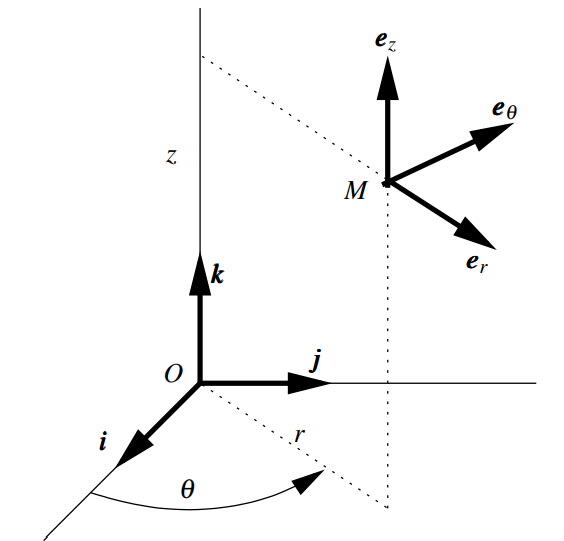
\includegraphics[width=0.5\textwidth]{\path/Coord_cyl}
\caption{Système de coordonnées cylindrique}
\label{fig:C_1}
\end{figure}
$$\begin{aligned}
&\er=\partial_{r}\OM=\cos\theta\vec{i}+\sin\theta\vec{j}\\
&\etheta=\dfrac{1}{r}\partial_{\theta} \OM=-\sin\theta\vec{i}+\cos\theta\vec{j}=\vec{k}\wedge \er\\
&\ez=\partial_{z}\OM=\vec{k}\\
\end{aligned}$$
Le point courant $M$ est défini par:
$$\OM=r\cos\theta\vec{i}+r\sin\theta\vec{j}+z\vec{k}=r\er+z\vec{k}$$
\subsection{Champs scalaires}
Soit $f$ un champ scalaire:
$$M\in \VV_{3}\overset{f}{\longmapsto}f(M)=f(r,\theta,z)\in \RR$$
Le gradient vaut:
$$\vgrad f=\partial_{r}f\er+\frac{1}{r}\partial_{\theta}f\etheta+\partial_{z}f\ez$$
\subsection{Champs vectoriels}
Soit $\vec{v}$ un champ vectoriel:
$$M\in \VV_{3}\overset{\vec{v}}{\longmapsto}\vec{v}(M)=v_{r}(r,\theta,z)\er +v_{\theta}(r,\theta,z)\etheta+v_{z}(r,\theta,z)\ez$$
alors:
\begin{equation}
\begin{aligned}
\left[(\tgrad \vec{v})_{\bullet\bullet}\right]&=
\begin{pmatrix}
\partial_{r}v_{r} & \dfrac{1}{r}\left(\partial_{\theta}v_{r}-v_{\theta}\right) & \partial_{z}v_{r}\\
\partial_{r}v_{\theta}& \dfrac{1}{r}\left(\partial_{\theta}v_{\theta}+v_{r}\right)& \partial_{z}v_{\theta}\\
\partial_{r}v_{z}& \dfrac{1}{r}\partial_{\theta}v_{z} & \partial_{z}v_{z}\\
\end{pmatrix}_{\{\er,\etheta,\ez\}}
\\
\div\vec{v}&=\partial_{r}v_{r}+\frac{1}{r} (\partial_{\theta} \vtheta+v_{r})+\partial_{z}v_{z}
\end{aligned}
\label{eq:formulaire_grad_cyl_vec}
\end{equation}
\subsection{Champs tensoriels du second ordre symétriques}
Soit $\ten{S}$ un champ tensoriel du second ordre \emph{symétrique}:
$$M\in \VV_{3}\overset{\ten{S}}{\longmapsto} \ten{S}(M)\in \Vsym_{3}$$
Les composantes de $\ten{S}$ dans la base orthonormée \{$\er,\etheta, \ez$\} forment la matrice symétrique:
$$\begin{pmatrix}
S_{rr}(r,\theta,z) & S_{r\theta}(r,\theta,z) & S_{rz}(r,\theta,z)\\
S_{r\theta}(r,\theta,z) & S_{\theta\theta}(r,\theta,z) & S_{\theta z}(r,\theta,z)\\
S_{rz}(r,\theta,z) & S_{\theta z}(r,\theta,z) & S_{zz}(r,\theta,z)
\end{pmatrix}_{\{\er,\etheta,\ez\}}$$
Le gradient de ce champ est un tenseur d'ordre 3 dont il n'est pas utile de détailler les 27 composantes sur la base physique. En revanche, les opérateurs qui suivent sont utiles en mécanique des milieux continus.\\

Le vecteur divergence de ce champ tensoriel est:
\begin{equation}
\begin{aligned}
\vdiv\ten{S}&=\left(\partial_{r}S_{rr}+\frac{1}{r}(\partial_{\theta}S_{r\theta}+S_{rr}-S_{\theta\theta})+\partial_{z}S_{rz}\right)\er\\
&\qquad +\left(\partial_{r}S_{r\theta}+\frac{1}{r}(\partial_{\theta} S_{\theta\theta}+2S_{r\theta})+\partial_{z}S_{\theta z}\right)\etheta\\
&\qquad +\left(\partial_{r}S_{rz}+\frac{1}{r}(\partial_{\theta}S_{\theta z}+S_{rz})+\partial_{z}S_{zz}\right)\ez
\end{aligned}
\label{eq:formulaire_div_cyl_ten}
\end{equation}
\section{Système de coordonnées sphériques}
Note importante Dans la littérature scientifique, il existe deux versions du système de coordonnées sphérique:
\begin{itemize}
\item dans la version présentée ici, l'angle $\phi$ est mesuré à partir du plan $(\e_{1},\e_{2})$. On pourrait les appeler \og coordonnées géographiques \fg{} ($\theta$ est la longitude, $\phi$ est la latitude, le plan $(\e_{1},\e_{2})$ est le plan équatorial). Le trièdre \{$\er,\etheta,\e_{\phi}$\} est direct;
\item dans l'autre version, l'angle $\Phi$ est mesuré sur le méridien de $M$ à partir du pôle Nord. On a donc:
$$\Phi=\frac{\pi}{2}-\phi\et \e_{\Phi}=-\e_{\phi}$$
On convertit aisément les formules avec les remplacements suivants:
$$\cos\phi\rightarrow\sin\Phi\et \sin\phi\rightarrow\cos\Phi$$
\end{itemize}
\subsection{Définition et notations}
Un point $M$ de l'espace est repéré par trois réels $r$, $\theta$ et $\phi$ définis sur la \figref{fig:C_2}. À chaque point $M$, on associe une base locale orthonormée \{$\er,\etheta,\e_{\phi}$\} définie par:
$$\begin{aligned}
&\er=\partial_{r}\OM=\cos\phi\vec{u}+\sin\phi\vec{k}=\cos\theta \cos\phi\vec{i}+\sin\theta \cos\phi\vec{j}+\sin\phi\vec{k}\\
&\etheta=\frac{\partial_{\theta}\OM}{r\cos\phi}=-\sin\theta\vec{i}+\cos\theta\vec{j}\\
&\e_{\phi}=\dfrac{\partial_{\phi}\OM}{r}=-\sin\phi\vec{u}+\cos\phi\vec{k}=-\cos\theta \sin\phi\vec{i}+\sin\theta \cos\phi\vec{j}+\sin\phi\vec{k}
\end{aligned}$$
\begin{figure}[h!]
\centering 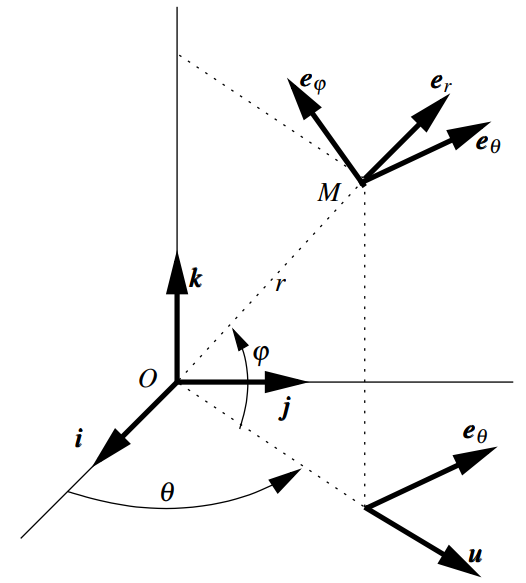
\includegraphics[width=0.5\textwidth]{\path/Coord_sphe.png}
\caption{Système de coordonnées sphériques}
\label{fig:C_2}
\end{figure}
Le point courant est:
$$\OM=r\cos\phi\cos\theta\vec{i}+r\cos\phi\sin\theta\vec{j}+r\sin\phi\vec{k}=r\er$$
\subsection{Champs scalaires}
Soit $f$ un champ scalaire:
$$M\in \VV_{3}\overset{f}{\longmapsto}f(M)=f(r,\theta,\phi)\in \RR$$
Le vecteur gradient s'écrit:
$$\vgrad f=\partial_{r}f\er+\dfrac{\partial_{\theta}f}{r\cos\phi}\etheta+\frac{\partial_{\phi}f}{r}\e_{\phi}$$
\subsection{Champs vectoriels}
Soit $\vec{v}$ un champ vectoriel:
$$M\in \VV_{3}\overset{\vec{v}}{\longmapsto}\vec{v}(M)=v_{r}(r,\theta,\phi)\er +\vtheta(r,\theta,\phi)\etheta+v_{\phi}(r,\theta,\phi)\e_{\phi}\in \VV_{3}$$
Les composantes du tenseur gradient dans la base orthonormée \{$\er,\etheta, \e_{\phi}$\} forment une matrice non symétrique:
\begin{equation}
\left[(\tgrad \vec{v})_{\bullet\bullet}\right]=\begin{pmatrix}
\partial_{r}v_{r} & \dfrac{1}{r\cos\theta}\partial_{\theta}v_{r}-\dfrac{1}{r}v_{\theta} & \dfrac{1}{r}\left(\partial_{\phi}v_{r}-v_{\phi}\right)\\
\partial_{r}v_{\theta} & \dfrac{1}{r\cos\phi}\left(\partial_{\theta}v_{\theta}-\sin\phi v_{\phi}\right)+\dfrac{1}{r}v_{r} & \dfrac{1}{r}\partial_{\phi}v_{\theta}\\
\partial_{r}v_{\phi} & \dfrac{1}{r\cos\phi}\left(\partial_{\theta}v_{\phi}+\sin\phi v_{\theta}\right) & \dfrac{1}{r}\left(\partial_{\phi}v_{\phi}+v_{r}\right)\\
\end{pmatrix}_{\{\er,\etheta,\ez\}}
\label{eq:formulaire_grad_sph_vec}
\end{equation}
La divergence est le scalaire:
$$\div\vec{v}=\partial_{r}v_{r}+\frac{\partial_{\theta}v_{\theta}-\sin\phi v_{\phi}}{r\cos\phi}+\frac{\partial_{\phi}v_{\phi}+2v_{r}}{r}$$
\subsection{Champs tensoriels du second ordre symétriques}
Soit $\ten{S}$ un champ tensoriel du second ordre \emph{symétrique}:
$$M\in \VV_{3}\overset{\ten{S}}{\longmapsto} \ten{S}(M)\in \mathbb{S}\subset \VV_{3}^{\otimes 2}$$
dont les composantes dans la base \{$\er,\etheta, \e_{\phi}$\} sont:
$$[(S)_{\bullet\bullet}]=\begin{pmatrix}
S_{rr}(r,\theta,\phi) & S_{r\theta}(r, \theta,\phi) & S_{r\phi}(r, \theta,\phi)\\
S_{r\theta}(r, \theta,\phi) & S_{\theta\theta}(r, \theta,\phi) & S_{\theta\phi}(r, \theta,\phi)\\
S_{r\phi}(r, \theta,\phi) & S_{\theta\phi}(r, \theta,\phi) & S_{\phi\phi}(r, \theta,\phi)
\end{pmatrix}_{\{\er,\etheta,\e_{\phi}\}} \quad \text{(matrice symétrique)}$$
Le gradient est un tenseur d'ordre 3 dont on ne détaille pas les 27 composantes. En revanche, les opérateurs qui suivent sont utiles en mécanique des milieux continus.

La divergence de ce champ tensoriel symétrique est le vecteur:
\begin{equation}
\begin{aligned}
\vdiv\ten{S}=&\left(\partial_{r}S_{rr}+\frac{\partial_{\theta}S_{r\theta}-\sin\phi S_{r\phi}}{r\cos\phi}+\frac{\partial_{\phi}S_{r\phi}+2S_{rr}-S_{\theta\theta}-S_{\phi\phi}}{r}\right)\er\\
&+\left(\partial_{r}S_{r\theta}+\frac{\partial_{\theta}S_{\theta\theta}-2\sin\phi S_{\theta\phi}}{r\cos\phi}+\frac{\partial_{\phi}S_{\theta\phi}+3S_{r\theta}}{r}\right)\etheta\\
&+\left(\partial_{r}S_{r\phi}+\frac{\partial_{\theta}S_{\theta\phi}+\sin\phi S_{\theta\theta}-\sin\phi S_{\phi\phi}}{r\cos\phi}+\frac{\partial_{\phi}S_{\phi\phi}+3S_{r\phi}}{r}\right)\e_{\phi}
\end{aligned}
\label{eq:formulaire_div_sph_ten}
\end{equation}
\chapter{Élasticité}\label{Chapitre:Elasticité}
\section*{\emph{Introduction}}
\begin{itemize}[label=$\star$]
\item A ce titre, nous introduisons tout d'abord à la \secref{Section:Élasticité dans l'hypothèse des petites perturbations} l'élasticité en petites perturbations, classiquement abordée en mécanique du solide \ldots pour immédiatement en souligner les limitations inhérentes à sa formulation.
\item Nous introduirons ensuite (\secref{Section:Élasticité en grandes transformations}), une loi de comportement élastique compressible en grandes transformations. Le choix concernant les invariants à utiliser pour la construction de ces modèles est immense, aussi nous ne présenterons qu'une poignée de comportements hyper-élastiques physiquement motivés.
\end{itemize}
%\clearpage
\section*{\emph{Définition}}
\begin{Defi}{Solide élastique}\label{Defi:Solide_elastique} On appelle comportement solide élastique, un modèle de milieu continu solide déformable tel que:
\begin{enumerate}[label=\arabic*)]
\item Dans toute évolution, la dissipation intrinsèque est nulle en toute particule et à tout instant:
\begin{equation}
\forall P \; \forall t,\quad \rho (T\dot{s}^{m}-\dot{e}^{m})+\SC:\TD=-\rho(\dot{\eHelm}^{m}+s^{m}\dot{T})+\SC:\TD=0
\label{Nullite_dissip_intrins_gen}
\end{equation}
\item Il n'y a pas de variable d'état interne dans la liste des variables d'état; les seules variables d'état sont donc:
\begin{itemize}[label=-]
\item la température $T$ (sa présence est imposée par la thermodynamique),
\item un tenseur de déformation actuelle $\DefoGen$ objectif (le milieu continu est un solide déformable),
%\item d'éventuelles directions actuelles d'anisotropie $\DirAnis^{i}$ (ou $\TenDirAnis_{t}^{(i)}$);
\end{itemize}
\item\label{point:3_defi_elast} Le tenseur des contraintes de Cauchy est une fonction d'état $\SC=f_{\SC}(T,\DefoGen)$donc indépendant de la vitesse de déformation actuelle $\TD)$
%$$\SC=f_{\SC}(T,\DefoGen,\TenDirAnis_{t}^{(1)}, \dots,\TenDirAnis^{(n)}_{t}) \; \text{(donc indépendant de la vitesse de déformation actuelle} \; \TD)$$
\end{enumerate}
\label{Defi_Solide_elast}
\end{Defi}
Ce modèle simple est assurément une idéalisation des matériaux réels, mais il est satisfaisant pour bon nombre de matériaux, tant que l'on ne dépasse pas certaines limites (apparition de phénomènes microscopiques dont l'effet est macroscopiquement notable). 
\clearpage
\section{Élasticité dans l'hypothèse des petites perturbations}\label{Section:Élasticité dans l'hypothèse des petites perturbations}
Malgré les limitations inhérentes à sa dérivation, il nous semble inenvisageable de commencer une présentation des lois élastiques sans mentionner l'élasticité traditionnelle de Hooke.\\
\begin{Hypothese}{des petites perturbations} Dans l'ensemble de cette \secref{Section:Élasticité dans l'hypothèse des petites perturbations}, nous retenons l'hypothèse, extrêmement restrictive des petites perturbations:
$$\Vert\tgrad_{L}\Dep\Vert\ll 1 \et T-T_{0}\ll 1$$
\end{Hypothese}
Autrement dit, le mouvement est une quasi-translation et les écarts de température à une valeur de référence sont infinitésimaux.
\subsubsection{Loi de comportement élastique linéaire}
La loi de comportement la plus simple relie linéairement la contrainte actuelle de Cauchy $\SC$ à la déformation linéarisée $\DefoHPP$ par l'intermédiaire d'un tenseur d'ordre 4 de \og rigidité \fg{} $\RigiLin$. Nous postulons que la relation entre le tenseur des contraintes et la déformation est donnée par (voir \cite{salenccon2005mecanique, forest2015mecanique}:
\begin{equation}
\SC = \RigiLin:\DefoHPP-\ten{k} \tau=\RigiLin:\GradSym(\Dep)-\ten{k} \tau
\label{eq:elasticité_lineaire_thermo}
\end{equation}
$\ten{k}$ désignant ici le tenseur de dilatation thermique, $\tau=T-T_{0}$ l'écart de température.
\paragraph{Matériau élastique isotrope} En supposant le matériau isotrope, le tenseur d'élasticité est entièrement caractérisé par deux scalaires \og mécanique \fg{} appelés \og coefficients de Lamé \fg{} $\lambda$ et $\mu$ ainsi qu'un scalaire \og thermique \fg{}:
\begin{equation}
k=\alpha(3\lambda+2\mu)=3\BulkModulus\alpha \text{ où }\alpha\text{ désigne le coefficient d’expansion thermique.}
\label{eq:defi_coeff_expansion_thermique}
\end{equation}
\begin{equation}
\SC = \left(\lambda\tr\DefoHPP-k\tau\right)\TU +2\mu\DefoHPP
\label{eq:elasticité_lineaire_thermo_iso}
\end{equation}
Cette loi s'écrit de manière complètement équivalente en séparant les parties déviatoriques et sphériques du tenseur des contraintes:
\begin{equation}
\SC = \left(\left(\lambda+\dfrac{2\mu}{3}\right)\tr\DefoHPP-k\tau\right)\TU +2\mu\dev\DefoHPP= \BulkModulus\left(\tr\DefoHPP-3\alpha\tau\right)\TU +2\mu\dev\DefoHPP=-p\TU+\devia
\label{eq:scission_lin_dev_sph_iso}
\end{equation}
Expression dans laquelle la décomposition moyenne/déviatorique d'un tenseur du second ordre est définie par:
$$\ten{X}=\underbrace{\left(\ten{X}-\dfrac{1}{3}\tr\ten{X}\right)}_{\dev\ten{X}}+\underbrace{\dfrac{1}{3}\tr\ten{X}}_{\mathrm{moy}\ten{X}}$$
Cette formulation est un petit peu plus appropriée pour les lois de comportement élasto-plastique car  la déformation plastique est purement déviatorique.\\

L'équation de la chaleur prend quand à elle la forme:
\begin{equation}
\rho C_{\varepsilon}\dot{T}+k T_{0}\tr\TD-k\Delta T=\PCaloVol
\label{eq:chaleur_HPP}
\end{equation}
$C_{\varepsilon}$ désigne la capacité thermique spécifique à déformation constante. Quelques ordres de grandeurs classiques pour les paramètres mises en jeu sont consignés dans le tableau p.186 de \cite{forest2015mecanique}.

\paragraph{Énergie libre associée}
La loi de comportement élastique linéaire en petites perturbations \eqref{eq:elasticité_lineaire_thermo} dérive de l'énergie libre de Helmholtz suivantes donnée par \citep{forest2015mecanique} p.184:
$$\SC=\dfrac{\partial \psi}{\partial \DefoHPP} \avec \psi =-\beta(T-T_{0})^{2}-3\BulkModulus\alpha(T-T_{0})\tr\DefoHPP+\dfrac{\lambda}{2}(\tr\DefoHPP)^{2}+\mu\DefoHPP:\DefoHPP$$
L'énergie libre peut s'écrit sous forme équivalent:
$$\begin{aligned}
\psi &=-\beta(T-T_{0})^{2}-3\BulkModulus\alpha(T-T_{0})\tr\DefoHPP+\dfrac{\lambda}{2}(\tr\DefoHPP)^{2}+\mu\DefoHPP:\DefoHPP\\
\psi &=-\beta(T-T_{0})^{2}-3\BulkModulus\alpha(T-T_{0})\tr\DefoHPP+\dfrac{\lambda}{2}(\tr\DefoHPP)^{2}+\mu\tr\left(\DefoHPP\cdot\DefoHPP\right)\\
\psi &=-\beta(T-T_{0})^{2}-3\BulkModulus\alpha(T-T_{0})\tr\DefoHPP+\dfrac{\lambda}{2}(\tr\DefoHPP)^{2}+\mu\pa{\dfrac{1}{3}\tr\DefoHPP\TU+\dev\DefoHPP}:\pa{\dfrac{1}{3}\tr\DefoHPP\TU+\dev\DefoHPP}\\
\psi &=-\beta(T-T_{0})^{2}-3\BulkModulus\alpha(T-T_{0})\tr\DefoHPP+\pa{\dfrac{\lambda}{2}+\dfrac{\mu}{3}}(\tr\DefoHPP)^{2}+\mu\dev\DefoHPP:\dev\DefoHPP\\
\psi &=-\beta(T-T_{0})^{2}\underbrace{-3\BulkModulus\alpha(T-T_{0})\tr\DefoHPP+\dfrac{\BulkModulus}{2}(\tr\DefoHPP)^{2}}_{\PsiVol}+\underbrace{\mu\dev\DefoHPP:\dev\DefoHPP}_{\psi ^{iso-vol}}\\
\end{aligned}$$
\section{Thermo-Élasticité en grandes transformations}\label{Section:Élasticité en grandes transformations}
Lorsque la transformation de la matière viole l'hypothèse des petites perturbations, la loi de Hooke devient caduc et doit être remplacée par une loi élastique en grandes transformations. De telles lois sont souvent appelées \og hyper-élastiques \fg{}, bien qu'elles n'aient rien \og d'hyper quoi que ce soit \fg{}. Il s'agit simplement de lois élastiques dans le cas général.
\subsection{Loi thermo-élastique de type Néo-Hookéen généralisée}
Le modèle Néo-Hookéen postule une énergie libre massique de la forme suivante:
$$\eHelmMass = U(J) + \dfrac{\mu}{2}\left(\BBarI -3\right)$$
La fonction $U(J)$ aussi appelée fonction de compressibilité admet dans la littérature de nombreuses expressions dont découle la loi d'état (voir \secref{Section:Loi d'état}). La loi thermo-élastique en grandes transformations suivante est implantée dans le code CHARON (pour les détails de sa dérivation, nous renvoyons le lecteur à \cite{simo2006computational}):
\begin{equation}
\SC=\tilde{K}_{0}\TU+\tilde{K}_{1}\dev\CGG \quad \tilde{K}_{0}=\BulkModulus\ln\frac{\J}{1+3\alpha(T-T_{0})}; \quad \tilde{K}_{1}=\frac{\mu_{0}}{\J^{\frac{5}{3}}}
\label{eq:loi_grand_transfo}
\end{equation}
Dans cette égalité:
\begin{itemize}
\item $\CGG=\GT\cdot\GT^{\top}$ désigne le tenseur de déformation de Cauchy-Green gauche.
\item $\J=\det\GT$ est le jacobien de la transformation et traduit physiquement la \emph{dilatation volumique} d'une particule.
\item $\alpha$ désigne le coefficient de dilatation volumique 
\item Les modules de compressibilité $\xi$ et de cisaillement $\mu$ {\it initiaux} sont:
$$\BulkModulus=\frac{E_{0}}{3(1-2\nu_{0})}; \qquad \mu_{0}=\frac{E_{0}}{2(1+\nu_{0})}$$
\end{itemize}
La loi de comportement Néo-Hookéenne généralisée présente naturellement une séparation moyenne/déviatorique de la contrainte $\SC = -p\TU+\devia$:
\begin{align}
p &= -\BulkModulus\ln\frac{\J}{1+3\alpha(T-T_{0})}\\\label{eq:devia_Neo_Hook}
\devia &= \frac{\mu_{0}}{\J^{\frac{5}{3}}}\dev\CGG
\end{align}
En linéarisant pour des transformations infinitésimales, cette loi se réduit à l'élasticité linéarisée précédemment développée.\\

L'équation de conservation de l'énergie est:
$$\begin{aligned}
\SC:\TD+\PCaloVol-\div_{E}\CourantChal&=\left(\dfrac{\rho_{0}}{\J}C_{p}-\dfrac{3\alpha^{2} T\BulkModulus\left(\J+3\alpha(T-T_{0})\right)}{\J\left(1+3\alpha(T-T_{0})\right)^{2}}\right)\dot{T}\\
&\qquad +\dfrac{\BulkModulus}{\J}\left(\ln\left(\dfrac{\J}{1+3\alpha(T-T_{0})}\right)+\dfrac{3\alpha T}{1+3\alpha(T-T_{0})}\right)\Configuration_{0}tDilatVol+\dfrac{\mu_{0}}{\J}\Glisss\dot{\Glisss}
\end{aligned}$$
Si nous supposons l'évolution adiabatique, nous pouvons réécrire cette équation sous la forme:
$$\SC:\TD+\PCaloVol-\dfrac{\d\mathscr{E}^{source}}{\dt}=C_{\tan}(T,\J)\dfrac{\d T}{\dt}$$
Le problème incrémental explicite, actualisant la température à chaque itération, est:
$$T_{n+1}=T_{n}+\dfrac{1}{C_{\tan}(T^{n},\J^{n})}\left(\Delta t\left(\SC:\TD+\PCaloVol\right)-\Delta\mathscr{E}^{source}(T^{n}, \J^{n}, \Glisss^{n})\right)$$
%\ToDo{Reformuler cette loi en considérant l'énergie sous la forme: $\eHelmMass = \dots +\mu_{0}\left(\BBarI-3\right)$}
\subsection{Loi thermo-élastique de type Mooney-Rivlin généralisée}
La loi thermo-élastique en grandes transformations suivante est implantée dans le code CHARON:
\begin{equation}
\SC=\tilde{K}_{0}\TU+\tilde{K}_{1}\dev\CGG+\tilde{K}_{2}\dev\left(\CGG^{2}-\tr(\CGG)\CGG\right)
\label{eq:loi_grand_transfo_MR}
\end{equation}
Expression dans laquelle $\tilde{K}_{0}$ est identique à \eqref{eq:loi_grand_transfo} et les coefficients $\tilde{K}_{1}$ et $\tilde{K}_{2}$ sont:

$$\tilde{K}_{1}=\dfrac{\mu_{0}+\alpha_{0}}{\J^{\frac{5}{3}}} \et \tilde{K}_{2}=-\dfrac{\alpha_{0}}{\J^\frac{7}{3}}$$
Cette loi est une correction d'ordre supérieure au modèle Néo-Hookéen généralisé précédemment présenté. Le déviateur de la contrainte est plus explicitement:
\begin{equation}
\devia=\dfrac{\mu_{0}+\alpha_{0}}{\J^{\frac{5}{3}}}\dev\CGG-\dfrac{\alpha_{0}}{\J^\frac{7}{3}}\dev\left(\CGG^{2}-\tr(\CGG)\CGG\right)
\label{eq:devia_MR}
\end{equation}

\section{Loi de comportement fluide}
Les fluides sont des milieux continus ne possédant aucune configuration de référence physiquement significative. L'usage d'un tenseur mesurant la déformation n'est donc pas pertinent. Nous renvoyons le lecteur à \cite{garrigues2017comportement} pour la justification de la construction de la loi de comportement des fluides simples. 
\begin{Hypothese}{Loi de comportement du fluide simple Newtonien} Nous appelons fluide Newtonien un milieu continu dont le comportement vérifie l'équation suivante:
$$\SC=(-p+k\tr(\TD))\TU+2\mu\dev\TD=\left(-p+\left(k-\frac{2\mu}{3}\right)\tr(\TD)\right)\TU+2\mu \TD$$
\end{Hypothese}
où
\begin{itemize}[label=-]
\item $p=-\rho^{2}(T\partial_{\rho}f_{s}-\partial_{\rho}f_{e})$ est une fonction d'état caractéristique du fluide simple appelée la pression thermodynamique;
\item $k(T,\rho)$ est la viscosité de volume, souvent considérée comme une constante ou seulement fonction de la température ou même parfois nulle (fluides de Stokes);
\item $\mu(T,\rho)$ est la viscosité isovolume ou viscosité de cisaillement ou viscosité dynamique, souvent considérée comme une constante ou seulement fonction de la température ou même parfois nulle (fluides non visqueux);
\item $\TD$ est le tenseur des taux de déformation défini en cinématique.
\end{itemize}
\begin{Hypothese}{}\label{Hyp:6_8} Afin d'obtenir un modèle simple et facile à identifier, on suppose que la compressibilité à température constante $\chi_{T}$ et la dilatation thermique à pression constante $\alpha_{p}$ sont des constantes: $\chi_{T}(T,p)=\chi_{0}$ et $\alpha_{p}(T,\rho)=\alpha_{0}$, \emph{sous réserve que sous ces hypothèses une fonction} $f_{\eHelm}$ \emph{existe}.
\end{Hypothese}
Dans ce cadre la pression thermodynamique est simplement égale à:
$$p=\frac{1}{\chi_{0}}\ln\frac{\rho}{\rho_{0}}+\frac{\alpha_{0}}{\chi_{0}}(T-T_{0})+p_{0}=-\frac{1}{\chi_{0}}\ln\det\GT+\frac{\alpha_{0}}{\chi_{0}}(T-T_{0})+p_{0}$$
\chapter{Retour radial analytique pour la plasticité}
\subsection{Le modèle élasto plastique de Von-Mises}
Le critère de Von-Mises compare une contrainte dite \og équivalente \fg{} $\sigma_{eq}=\sqrt{\dfrac{3}{2}}\Vert \devia-\ten{X}\Vert$ à une valeur limite $\sigma_{0}(p)$. $\ten{X}$ désigne ici le centre du convexe d'élasticité, $p$ la plasticité cumulée définie par et $\devia$ le déviateur du tenseur des contraintes $\SC$. Le critère de Von-mises \emph{borne la norme du déviateur des contraintes} \cite{maitournam2017materiaux} par l'intermédiaire de la déformation plastique. Pour garantir l'admissibilité thermodynamique du modèle, nous choisissons de nous placer dans le cadre standard généralisé. Il s'agit de dériver l'évolution de la variable plastique d'un (pseudo-) potentiel de dissipation convexe par rapport au taux $\dot{\DefoHPP}^{p}$.

Introduisons la fonction de charge suivante:
$$\FChargeConvexe(\devia)=\sqrt{\frac{3}{2}}\Vert \devia-\ten{X}\Vert-\sigma_{0}$$
L'évolution de la déformation plastique est postulée sous la forme:
\begin{equation}
\dot{\DefoHPP}^{p}=\lambda\dfrac{\partial\FChargeConvexe(\devia)}{\partial\devia}=\lambda\sqrt{\dfrac{3}{2}}\dfrac{\devia}{\Vert \devia\Vert}, \avec \lambda\geq 0, \FChargeConvexe\leq 0, \lambda \FChargeConvexe=0
\label{eq:evolution variable_interne}
\end{equation}
Le multiplicateur de Lagrange $\lambda$ assure les conditions de Kuhn-Tucker standards:
\begin{itemize}
\item soit la contrainte se situe dans le convexe d'élasticité $\FChargeConvexe(\FthEpsp)< 0$ et la déformation plastique demeure constante,
\item soit le critère est saturé $\FChargeConvexe(\FthEpsp)=0$ et la déformation plastique évolue de manière à maintenir la contrainte sur la frontière du domaine d'élasticité.
\end{itemize}
\subsubsection{Équations générales avec un écrouissage cinématique linéaire}
Le problèmes élasto-plastique en petites perturbations avec un critère de Von-Mises avec écrouissage cinématique linéaire est régi par le jeu de potentiel et d'équations suivantes:
\begin{itemize}
\item Potentiel thermodynamique:
$$\rho \eHelm(\DefoHPP,\EpsP)=\frac{1}{2}(\DefoHPP-\EpsP):\RigiLin:(\DefoHPP-\EpsP)+\frac{1}{2}\EpsP:\TenEcroui:\EpsP$$
\item Lois de comportement
$$\SC =\RigiLin:(\DefoHPP-\EpsP)$$
\item Force thermodynamique motrice de la plasticité
$$\FthEpsp=\dev(\SC-\TenEcroui:\EpsP)=\devia-\TenTranslatDom$$
avec $\TenTranslatDom=\TenEcroui:\EpsP=\frac{2}{3}C\EpsP$, tenseur déviatorique.
\item Lois complémentaires:
$$\begin{aligned}
\dot{\DefoHPP}^{p}&=\lambda\frac{\partial \FChargeConvexe(\FthEpsp)}{\partial \FthEpsp}=\lambda\sqrt{\frac{3}{2}}\frac{\devia-\TenTranslatDom}{\Vert \devia-\TenTranslatDom\Vert} \quad \avec \lambda\geq 0, \FChargeConvexe\leq 0, \lambda\FChargeConvexe=0\\
\FChargeConvexe(\FthEpsp)&=\FChargeConvexe(\devia-\TenTranslatDom)=\sqrt{\frac{3}{2}}\Vert \devia-\TenTranslatDom\Vert-\sigma_{0}
\end{aligned}$$
\item Puissance dissipée: $\dint=\FthEpsp:\dot{\DefoHPP}^{p}=(\devia-\TenTranslatDom):\dot{\DefoHPP}^{p}= \sigma_{0}\dot{p}.$
\end{itemize}
\subsubsection{Équations générales avec un écrouissage isotrope}
Le problèmes élasto-plastique en petites perturbations avec un critère de Von-Mises avec écrouissage isotrope est régi par le jeu de potentiel et d'équations suivantes:
\begin{itemize}
\item Potentiel thermodynamique:
$$\rho \eHelm(\DefoHPP,\EpsP)=\frac{1}{2}(\DefoHPP-\EpsP):\RigiLin:(\DefoHPP-\EpsP)+\eHelm_{p}(p)$$
\item Lois de comportement
$$\SC =\RigiLin:(\DefoHPP-\EpsP)$$
\item Force thermodynamique motrice de la plasticité
$$\begin{aligned}
\FthEpsp&=\dev(\SC)=\devia\\
A_{p}
\end{aligned}$$
\item Lois complémentaires:
$$\begin{aligned}
\dot{\DefoHPP}^{p}&=\lambda\frac{\partial \FChargeConvexe(\FthEpsp)}{\partial \FthEpsp}=\lambda\sqrt{\frac{3}{2}}\frac{\devia}{\Vert \devia\Vert} \quad \avec \lambda\geq 0, \FChargeConvexe\leq 0, \lambda\FChargeConvexe=0\\
\FChargeConvexe(\FthEpsp)&=\sqrt{\frac{3}{2}}\Vert \devia\Vert-\sigma_{0}+R(p)
\end{aligned}$$
\item Puissance dissipée: $\dint=\FthEpsp:\dot{\DefoHPP}^{p}=(\devia-\TenTranslatDom):\dot{\DefoHPP}^{p}= \sigma_{0}\dot{p}.$
\end{itemize}
\subsection{Problème incrémental pour un matériau élasto-plastique à écrouissage cinématique linéaire}
On considère le problème d'évolution précédent, sur l'intervalle $[0,T]$. Le temps est discrétisé en $N+1$ instants, $0=t_{0}<t_{1} <\cdots<t_{n}<t_{n+1}=t_{n}+\Delta t<\cdots<t_{N}=T.$\\

La théorie présentée ci-dessous est directement tirée de \cite{maitournam2017materiaux}.\\

On suppose que l'état est connu à l'instant $t_{n}$, noté $\{\DefoHPP_{n},\DefoHPP_{n}^{p},\SC_{n},\FthEpsp_{n}\}$. Il est en équilibre avec le chargement noté $F_{n}^{\mathrm{g}}$. On effectue un incrément de chargement $\Delta F^{\mathrm{g}}$, et on cherche la solution à l'instant $t_{n+1}$. On choisit d'emblée une méthode implicite de résolution qui consiste à imposer qu'à l'instant $t_{n+1}$, les équations d'équilibre et les lois complémentaires sont vérifiées. Les equations du problème s'écrivent alors:
\begin{align}
&\left\{\begin{aligned}
&\vdiv\SC_{n+1}+\rho\FMass_{n+1}=\vec{0} \sur \Omega\\
&\sigma_{ij(n+1)}n_{j}=T_{i(n+1)}^{\mathrm{g}}\sur S_{T_{i}}, i=1, 2, 3\\	
\end{aligned}\right.\\\label{eq:loi_compo_increm_cin_lin}
&\left\{\begin{aligned}
&\SC_{n+1}=\RigiLin:(\DefoHPP-\EpsP)\\
&\FthEpsp_{n+1}=\devia_{n+1}-\CentreConv_{n+1}\\
\end{aligned} \right. \avec\CentreConv=H \DefoHPP^{p}=\frac{2}{3}C\EpsP\et \devia=\dev\SC\\\label{eq:Fonction_charge_incre}
&\FChargeConvexe(\FthEpsp_{n+1})=\FChargeConvexe(\devia_{n+1}-\CentreConv_{n+1})=\sqrt{\frac{3}{2}}\Vert \devia_{n+1}-\CentreConv_{n+1}\Vert-\sigma_{0}\leq0\\\label{eq:Ecoulement_incre}
&\DeltaDefoHPP^{p}=\lambda^{\star}\frac{\FthEpsp_{n+1}}{\Vert \FthEpsp_{n+1}\Vert} \quad \avec \lambda^{\star}\geq 0, \quad \FChargeConvexe(\FthEpsp_{n+1})\leq 0 \quad \lambda^{\star}\FChargeConvexe(\FthEpsp_{n+1})=0\\
&u_{i(n+1)}=u_{i(n+1)}^{\mathrm{g}} \sur S_{u_{t}}, i=1, 2, 3.\\
&\avec: \; \lambda^{\star}=\lambda\Delta t
\end{align}
Le champ de déplacement peut être pris comme l'inconnue principale du problème. En effet, comme on le montre par la suite, la connaissance de l'incrément de déformation permet, par un calcul local, de déterminer en tout point l'incrément de déformation plastique. Le principe d'un schéma de résolution itératif consiste à:
\begin{enumerate}
\item partir de l'état à l'instant $t_{n}$ supposé connu; initialiser les incréments de déformation et de déformation plastique à zéro;
\item calculer le résidu à l'instant $t_{n+1}$ (l'écart entre les efforts intérieurs et les efforts extérieurs); s'il est inférieur à une tolérance fixée, arrêter le processus car la convergence est atteinte, sinon passer à l'étape suivante;
\item corriger (actualiser) l'incrément de déplacement en résolvant un problème linéaire impliquant le résidu précédent;
\item utiliser l'incrément de déplacement calculé précédemment, pour calculer les incréments des déformations plastiques (ou des variables dissipatives) grâce aux lois d'évolution (à $t_{n+1}$), puis les contraintes et les autres forces thermodynamiques grâce aux lois d'état.
\end{enumerate}
\subsubsection{Calcul de l'incrément de la déformation plastique à partir de celui de la déformation}
Dans cette section, on considère la dernière étape du schéma de résolution précédent. L'incrément de déplacement entre les instants $t_{n}$ et $t_{n+1}$ est supposé connu. En fonction de celui-ci et de l'état à l'instant $t_{n}$, on va calculer l'incrément de déformation plastique. Pour cela, on utilise les équations \eqref{eq:Fonction_charge_incre},\eqref{eq:Ecoulement_incre}.\\
\begin{Not}{Incréments de déformation} Nous notons respectivement $\DeltaDefoHPP$, $\DeltaDefoHPP_{d}$ et $\DeltaEpsP$ les incréments de déformations totales, de déformations totales déviatoriques et de déformations plastiques:
$$\DeltaDefoHPP = \DefoHPP_{n+1}-\DefoHPP_{n}; \quad \DeltaDefoHPP_{d}=\dev\DeltaDefoHPP; \quad \DeltaEpsP=\EpsP_{n+1}-\EpsP_{n}$$
\end{Not}
\begin{Theo}{Incrément de déformation plastique}L'incrément de déformation plastique est colinéaire à un tenseur fonction uniquement de l'incrément de déformation $\DeltaDefoHPP=\DefoHPP_{n+1}-\DefoHPP_{n}$ et de l'état à $t_{n}.$ 
\end{Theo}
\begin{Demo}{Nous savons déjà que l'incrément de déformation plastique est donné, d'après \eqref{eq:Ecoulement_incre}, par:
$$\DeltaEpsP=\lambda^{\star}\frac{\FthEpsp_{n+1}}{\Vert \FthEpsp_{n+1}\Vert}$$
Il suffit donc de prouver que le multiplicateur plastique $\lambda^{\star}$ et la force thermodynamique $\FthEpsp_{n+1}$ peuvent s’exprimer en fonction uniquement de l'incrément de déformation $\DeltaDefoHPP=\DefoHPP_{n+1}-\DefoHPP_{n}$ et de l'état à $t_{n}$.\\

La force thermodynamique $\FthEpsp_{n+1}$ est ici égale à:
$$\begin{aligned}
\FthEpsp_{n+1}&=\devia_{n+1}-\CentreConv_{n+1} \quad \eqref{eq:loi_compo_increm_cin_lin}\\
&=2\mu(\dev\DefoHPP_{n+1}-\EpsP_{n+1})-H\EpsP_{n+1} \quad \eqref{eq:loi_compo_increm_cin_lin}\et \EpsP_{n+1} \; \text{déviatorique}\\
&=\devia_{n}+2\mu(\DeltaDefoHPP_{d}-\DeltaEpsP)-H(\EpsP_{n}+\DeltaEpsP) \\
&=\devia_{n}-H\DefoHPP_{n}^{p}+2\mu\DeltaDefoHPP_{d}-(2\mu+H)\DeltaEpsP
\end{aligned}$$
En posant:
\begin{equation*}
\FthEpsp_{n+1}^{\text{elas}}=\devia_{n}-H\DefoHPP_{n}^{p}+2\mu\DeltaDefoHPP_{d} \quad \et \quad \hat{\ten{n}}_{n+1}^{\text{elas}}=\frac{\FthEpsp_{n+1}^{\text{elas}}}{\Vert\FthEpsp_{n+1}^{\text{elas}}\Vert}
\end{equation*}
$\FthEpsp_{n+1}^{\text{elas}}$ est fonction uniquement de l'incrément de déformation $\DeltaDefoHPP=\DefoHPP_{n+1}-\DefoHPP_{n}$ et de l'état à $t_{n}$. On peut alors écrire $\FthEpsp_{n+1}$ comme:
\begin{align}
\FthEpsp_{n+1}&=(\devia_{n}-H\DefoHPP^{p}_{n}+2\mu\DeltaDefoHPP_{d})-(2\mu+H)\lambda^{\star}\frac{\FthEpsp_{n+1}}{\Vert\FthEpsp_{n+1}\Vert}\\\label{eq:colin_fth_fth_elas}
\implique \FthEpsp_{n+1} &= \FthEpsp_{n+1}^{\text{elas}}-(2\mu+H)\lambda^{\star}\frac{\FthEpsp_{n+1}}{\Vert\FthEpsp_{n+1}\Vert}
\end{align}
On en déduit que $\FthEpsp_{n+1}$ et $\FthEpsp_{n+1}^{\text{elas}}$ sont colinéaires et donc $\hat{\ten{n}}_{n+1}^{\text{elas}}=\hat{\ten{n}}_{n+1}$. Par conséquent:
\begin{equation}
\DeltaEpsP=\lambda^{\star}\frac{\FthEpsp_{n+1}}{\Vert\FthEpsp_{n+1}\Vert}=\lambda^{\star}\hat{\ten{n}}^{\text{elas}}_{n+1}
\label{eq:6_80}
\end{equation}
Pour déterminer $\lambda^{\star}$, on utilise l'équation $\FChargeConvexe(\FthEpsp_{n+1})=0$ avec l'expression \eqref{eq:colin_fth_fth_elas} de $\FthEpsp_{n+1}$:
$$\begin{aligned}
\FChargeConvexe(\FthEpsp_{n+1})=0\implique \sqrt{\frac{2}{3}}\sigma_{0} &= \Vert A_{n+1}^{\text{elas}}-(2\mu+H)\lambda^{\star}\hat{\ten{n}}_{n+1}\Vert\\
\sqrt{\frac{2}{3}}\sigma_{0}&=\left\Vert\FthEpsp_{n+1}^{\text{elas}}\left(1-\frac{(2\mu+H)\lambda^{\star}}{\Vert\FthEpsp_{n+1}^{\text{elas}}\Vert}\right)\right\Vert\\
\sqrt{\frac{2}{3}}\sigma_{0}&=\Vert\FthEpsp_{n+1}^{\text{elas}}\Vert-(2\mu+H)\lambda^{\star}
\end{aligned}$$
D'où\footnote{ En effet, de l'équation \eqref{eq:colin_fth_fth_elas}, on déduit que: $\Vert \FthEpsp_{n+1}\Vert+(2\mu+H)\lambda^{\star}=\Vert\FthEpsp_{n+1}^{\text{elas}}\Vert$, ce qui permet de voir que $\Vert\FthEpsp_{n+1}^{\text{elas}}\Vert-(2\mu+H)\lambda^{\star}\geq 0.$}
$$ \lambda^{\star}=\frac{\Vert \FthEpsp_{n+1}^{\text{elas}}\Vert-\sqrt{\frac{2}{3}}\sigma_{0}}{2\mu+H}$$
Finalement, on obtient l'expression suivante de $\DeltaEpsP$, valable dans tous les cas:
\begin{equation}
\DeltaEpsP=\frac{\langle\Vert\FthEpsp_{n+1}^{\text{elas}}\Vert-\sqrt{\frac{2}{3}}\sigma_{0}\rangle}{2\mu+H}\hat{\ten{n}}_{n+1}^{\text{elas}}
\label{eq:Correction_plastique_incre}
\end{equation}
}\end{Demo}
Ainsi en un point donné, à partir de l'état à l'instant $t_{n}$ suppose connu, si $\DeltaDefoHPP$ est donné, on détermine l'état à l'instant $t_{n+1}$ par l'algorithme qui suit, dit algorithme de retour radial.
\paragraph{Algorithme 1: Retour radial dans le cas de l'écrouissage cinématique linéaire\\}
\begin{enumerate}
\item On effectue une première estimation de l'état en supposant que l'évolution est élastique
$$\DeltaSC^{\text{elas}}=\RigiLin:\DeltaDefoHPP, \quad \SC_{n+1}^{\text{elas}}=\SC_{n}+\RigiLin:\DeltaDefoHPP \quad \text{et} \; \devia^{\text{elas}}_{n+1}=\dev\SC^{\text{elas}}_{n+1}.$$
\item On calcule: $\FthEpsp_{n+1}^{\text{elas}}=\devia_{n+1}^{\text{elas}}-H\DefoHPP_{n}^{p}=\devia_{n}+2\mu\DeltaDefoHPP_{d}-H\DefoHPP^{p}_{n}$
\begin{center}
et: $\FChargeConvexe(\FthEpsp_{n+1}^{\text{elas}})=\sqrt{\frac{3}{2}}\Vert\FthEpsp_{n+1}^{\text{elas}}\Vert-\sigma_{0}.$
\end{center}
\item SI $\FChargeConvexe(\FthEpsp_{n+1}^{\text{elas}})\leq 0$, alors l'évolution est élastique,\\

SINON l'incrément de la déformation plastique est donné par la formule \eqref{eq:Correction_plastique_incre}:
$$\DeltaEpsP=\frac{\langle\Vert\FthEpsp_{n+1}^{\text{elas}}\Vert-\sqrt{\frac{2}{3}}\sigma_{0}\rangle}{2\mu+H}\frac{\vec{\FthEpsp}_{n+1}^{\text{elas}}}{\Vert \FthEpsp_{n+1}^{\text{elas}}\Vert}.$$
\end{enumerate}
Cet algorithme de retour radial, doit sa dénomination au fait que l'incrément de déformation plastique $\DeltaEpsP$ est obtenu par projection orthogonale de la contrainte-test généralisée $\FthEpsp_{n+1}^{\text{elas}}$ sur le convexe actuel d'élasticité défini par $\FChargeConvexe(\FthEpsp) \leq 0$. Ainsi, la loi de comportement est vérifiée à l'instant $t_{\mathrm{n}+1}:\FChargeConvexe(\FthEpsp_{n+1})=0$ et $\DeltaEpsP$ est normal au critère de plasticité.
\begin{figure}[!h]
\begin{subfigure}[b]{0.49\textwidth}
\centering 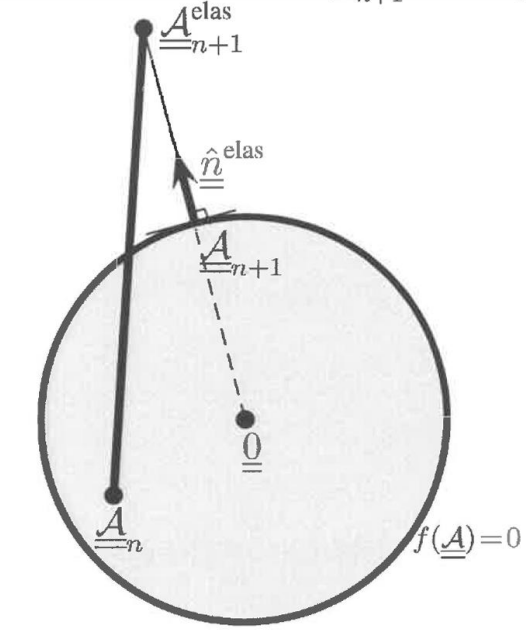
\includegraphics[width=0.8\textwidth]{\path/retour_rad_1}
\caption{Espace des forces $\FthEpsp$}
\end{subfigure}
\begin{subfigure}[b]{0.49\textwidth}
\centering 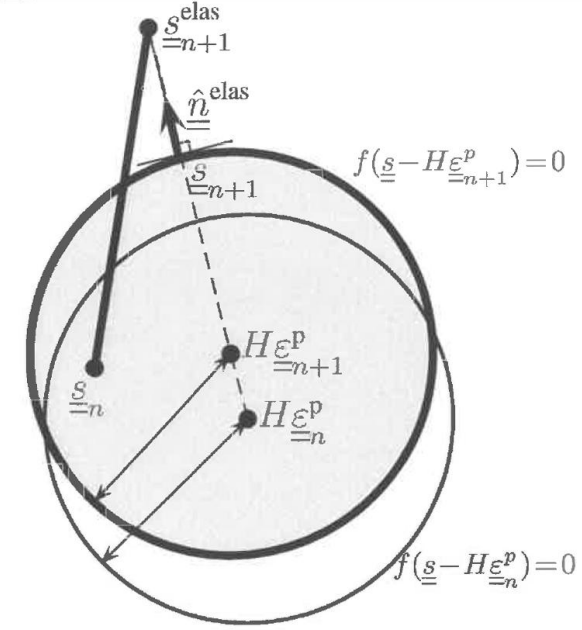
\includegraphics[width=0.8\textwidth]{\path/retour_rad_2}
\caption{Espace des déviateurs de contrainte}
\end{subfigure}
\caption{Illustration géométrique du \og retour radial \fg{} (projection orthogonale) dans le cas d'un modèle élasto-plastique de type von Mises à écrouissage cinématique linéaire. Figures issues de \cite{maitournam2017materiaux}}
\end{figure}
\subsection{Problème incrémentale écrouissage isotrope}
Nous montrons comment implémenter un problème élasto-plastique avec un critère de von Mises et un écrouissage linéaire isotrope. La mise à jour de la déformation plastique a, dans ce cas, une expression analytique. 
\subsubsection{Position du problème}
La réponse de la structure est calculée en utilisant un algorithme itératif de prédiction-correction basé sur le retour radial intégré dans une boucle globale de Newton-Raphson pour garantir. En raison de l'expression simple du critère de von Mises, la procédure de retour radial est entièrement analytique (avec un durcissement isotrope linéaire).
\subsubsection{Comportement élastoplastique}
Le matériau obéit à une loi élasto-plastique de Von-Mises isotrope avec une limite d'élasticité $\sigY$ et un durcissement isotrope de module $H$. Le comportement élastique est linéaire isotrope :
$$\SC = \lambda \tr(\DefoHPP-\EpsP)\bI + 2\mu(\DefoHPP-\EpsP) = \RigiLin:(\DefoHPP-\EpsP)$$
La fonction de charge est donnée par:
$$\FChargeConvexe(\SC) = \sqrt{\frac{3}{2}\devia:\devia} - \sigY -Hp \leq 0$$
où $\devia = \dev(\SC)$ est la contrainte déviatorique et $p$ est la déformation plastique équivalente cumulée telle que $\dot{p} = \sqrt{\frac{2}{3}}|\dot{\DefoHPP}^{p}|$. Nous introduisons également la contrainte équivalente de von Mises :
$$\sigma_{eq} =  \sqrt{\frac{3}{2}\devia:\devia}$$
L'écoulement plastique est donnée par la règle associée :
$$\dot{\DefoHPP}^{p} = \dot{\lambda}\dfrac{\partial\FChargeConvexe}{\partial \SC}$$
ce qui donne dans le cas présent :
\begin{equation}
\dot{\DefoHPP}^{p} = \dot{p}\dfrac{3}{2\sigma_{eq}}\devia
\label{eq:flow-rule}
\end{equation}
\subsubsection{Algorithme de prédiction-correction pour l'intégration du comportement constitutif}
La procédure de retour radial consiste à trouver une nouvelle contrainte $\SC_{n+1}$ et une variable interne $p_{n+1}$ vérifiant le critère de plasticité courant à partir d'une contrainte précédente $\SC_{n}$, d'une variable interne $p_n$ et d'une incrémentation de déformation totale $\Delta \DefoHPP$. Nous adoptons les notations de \cite{bonnet2014finite}.

Pour une évolution plastique, la règle d'écoulement \eqref{eq:flow-rule} est approchée à $t_{n+1}$ en utilisant une approximation implicite:
\begin{equation}
\Delta \EpsP = \Delta p \dfrac{3}{2\sigma_{\text{eq},n+1}}\devia_{n+1}
\label{flow-rule-incr}
\end{equation}
Une contrainte élastique test $\SC_{\text{elas}} = \SC_{n} + \CC:\Delta \DefoHPP$ est d'abord calculée. Le critère de plasticité est ensuite évalué avec la déformation plastique précédente $\FChargeConvexe^{\text{elas}} = \sigma_{eq}^{\text{elas}} - \sigY - H p_n$ où $\sigma_{eq}^{\text{elas}}$ est la contrainte équivalente de von Mises de la contrainte élastique d'essai.
\begin{itemize}
\item Si $\FChargeConvexe^{\text{elas}} < 0$, la déformation plastique n'évolue pas, $\Delta p=0,\Delta  \EpsP =\ten{0}$ et $\SC_{n+1} = \SC_\text{elas}$.
\item Sinon, la plasticité évolue et l'incrément de déformation plastique $\Delta p$ est tel que:
\begin{align}
\label{plastic-ev-discr}
\SC_{n+1} &= \SC_\text{elas} - 2\mu\Delta \EpsP\\
\Delta \EpsP &= \Delta p \dfrac{3}{2\sigma_{\text{eq},n+1}}\devia_{n+1}\\
\FChargeConvexe(\SC_{n+1}) &= \sigma_{\text{eq},n+1} - \sigY - H p_n - H\Delta p = 0
\end{align}
\end{itemize}
En prenant la partie déviatorique de la première équation de \eqref{plastic-ev-discr} et en injectant dans la deuxième, on montre que :
$$\left(1+\dfrac{3\mu\Delta p}{\sigma_{\text{eq},n+1}}\right)\devia_{n+1} = \devia_\text{elas}$$
ce qui se traduit par
$$\sigma_{\text{eq},n+1} = \sigma_{eq}^\text{elas} - 3\mu \Delta p$$
En remplaçant dans la troisième équation de \eqref{plastic-ev-discr}, on déduit la valeur de l'incrément de déformation plastique cumulée :
$$\Delta p = \dfrac{\FChargeConvexe^\text{elas}}{3\mu+H}$$
et l'incrément de déformation plastique en utilisant les relations précédentes :
$$\Delta \EpsP = \Delta p \dfrac{3}{2\sigma_{\text{eq},n+1}}\devia_{n+1} = \Delta p \dfrac{3}{2\sigma_{eq}^\text{elas}}\devia_\text{elas}$$
Ainsi, aussi bien un évolution élastique que plastique peut être prise en compte en définissant l'incrément de déformation plastique comme suit :
\begin{equation}
\Delta p = \dfrac{\langle \FChargeConvexe^\text{elas}\rangle_+}{3\mu+H}
\label{Deltap-formula}
\end{equation}
où $\langle \star \rangle_+$ désigne la partie positive de $\star$.

\chapter{Problème statique}
Le code CHARON possède également un solveur dédié à la résolution de problème quasi-statique. Dans ce cas, notamment pour l'endommagement, un algorithme échelonné est utilisé pour résoudre les problèmes d'endommagement.
\section{Accélération d'Anderson-Sur relaxation pour les problèmes endommageables quasi-statique}
Cette section détaille la procédure d'accélération de point fixe donnée dans METTRE REF An accelerated staggered scheme for variational phase-field models of brittle fracture.

L’accélération d'Anderson est un algorithme permettant significativement d’améliorer le taux de convergence de l'algorithme échelonné au voisinage de la solution. Une profondeur de $m=1$ est choisie. 
\begin{Not}{Pas et itération} Nous notons avec un sous-script \og $k$ \fg{} le $n^{\text{ème}}$ pas de chargement et avec l'exposant \og $i$ \fg{} l'itération courante. De plus nous notons $\vec{x}=\begin{Bmatrix}
\Dep\\
d
\end{Bmatrix}$ le vecteur \og inconnus généralisées\fg{}.
\end{Not}
\subsection{Accélération d'Anderson}
Pour illustrer la procédure, supposons que nous commençons un nouveau pas de chargement d'indice $n$ initialisé avec le vecteur $\vec{x}_{n}^{0}=\begin{Bmatrix}
\Dep_{n}^{0}\\
d_{n}^{0}
\end{Bmatrix}$. 
\begin{itemize}
\item Nous entamons la première itération: $i=1$. A l’issue du calcul en déplacement et en endommagement, nous obtenons un nouveau vecteur solution $\vec{x}_{n}^{1}$.
\begin{itemize}
\item Si la convergence à lieu, nous initialisons un nouveau pas de calcul, 
\item Sinon, nous calculons $\Delta\Ss(\vec{x}_{n}^{0})=\vec{x}_{n}^{1}-\vec{x}_{n}^{0}$ et lançons une nouvelle itération.
\end{itemize}
\item La deuxième itération: $i=2$, fournit une nouvelle solution $\vec{x}_{n}^{2}$. 
\begin{itemize}
\item Si le test de convergence est concluant, nous acceptons la solution $\vec{x}_{n}^{2}$, et initialisons un nouveau pas de calcul,
\item  si le calcul n'est pas convergé en revanche, nous calculons:
$$\Delta\Ss(\vec{x}_{n}^{1})=\vec{x}_{n}^{2}-\vec{x}_{n}^{1}$$
Puis nous cherchons $\alpha\in\RR$, tel que:
$$\min_{\alpha\in\RR}f(\alpha) \avec f(\alpha)=\left\Vert\alpha\Delta\Ss(\vec{x}_{n}^{0})+(1-\alpha)\Delta\Ss(\vec{x}_{n}^{1})\right\Vert_{2}^{2}$$
Le minimum de $f$ est analytique car il s'agit d'une fonction quadratique:
$$\begin{aligned}
f(\alpha)&=\left(\alpha\Delta\Ss_{0}+(1-\alpha)\Delta\Ss_{1}\right)\cdot\left(\alpha\Delta\Ss_{0}+(1-\alpha)\Delta\Ss_{1}\right)\\
&=\alpha^{2}\Delta\Ss_{0}^{2}+2\alpha(1-\alpha)\Delta\Ss_{0}\cdot\Delta\Ss_{1}+(1-\alpha)^{2}\Delta\Ss_{1}^{2}\\
&=\alpha^{2}\left(\Delta\Ss_{0}^{2}-2\Delta\Ss_{0}\cdot\Delta\Ss_{1}+\Delta\Ss_{1}^{2}\right)+2\alpha\left(\Delta\Ss_{0}\cdot\Delta\Ss_{1}-\Delta\Ss_{1}^{2}\right)+\Delta\Ss_{1}^{2}\\
&=\alpha^{2}\left(\Delta\Ss_{0}-\Delta\Ss_{1}\right)^{2}+2\alpha\Delta\Ss_{1}\cdot\left(\Delta\Ss_{0}-\Delta\Ss_{1}\right)+\Delta\Ss_{1}^{2}\\
\end{aligned}$$
Le minimum de cette fonction quadratique est obtenue pour:
$$\alpha_{\min}=\dfrac{\Delta\Ss_{1}\cdot\left(\Delta\Ss_{1}-\Delta\Ss_{0}\right)}{\left(\Delta\Ss_{1}-\Delta\Ss_{0}\right)^{2}}=\dfrac{\left(\vec{x}_{n}^{2}-\vec{x}_{n}^{1}\right)\cdot\left(\vec{x}_{n}^{2}-2\vec{x}_{n}^{1}+\vec{x}_{n}^{0}\right)}{\left(\vec{x}_{n}^{2}-2\vec{x}_{n}^{1}+\vec{x}_{n}^{0}\right)\cdot \left(\vec{x}_{n}^{2}-2\vec{x}_{n}^{1}+\vec{x}_{n}^{0}\right)}$$
\begin{Rem}{Nous pouvons retrouver ce résultats en cherchant la valeur $\alpha_{\min}$ qui annule $\dfrac{\d}{\d\alpha}\left(\alpha\Delta\Ss_{0}+(1-\alpha)\Delta\Ss_{1}\right)^{2}$}\end{Rem}
nous lançons alors une nouvelle itération avec la solution \og accélérée \fg{}:
$$\vec{x}_{n}^{2}=\alpha \vec{x}_{n}^{1}+(1-\alpha)\vec{x}_{n}^{2}$$ 
\item Pour la suite, nous suivons alors toujours le même schéma.
\end{itemize}
\end{itemize}

\chapter{Schéma de Runge Kutta}
Les schémas de Runge-Kutta sont une famille de méthodes numériques utilisées pour résoudre des équations différentielles ordinaires. Ce sont des méthodes itératives qui approchent la solution d'une équation différentielle en évaluant une ou plusieurs fois la fonction à plusieurs points intermédiaires dans chaque intervalle. Ces méthodes offrent généralement une meilleure précision que les méthodes d'Euler simples, tout en maintenant une relative facilité d'implémentation. Cette annexe leurs est dédiée.
\section{Schéma de Runge-Kutta pour les équations différentielles d'ordre 1}
Nous cherchons à résoudre l'équation différentielle 
\begin{equation}
\dot{y} = f(t,y)
\label{eq:EDO_ordre_1}
\end{equation}
sur un intervalle de temps $t\in[t_{0},t_{f}]$ avec les conditions initiales données $y_{0}$, $\dot{y}_{0}$.
\subsection{Schéma de Runge-Kutta d'ordre 1 ou méthode d'Euler-Explicite}
Le schéma de Runge-Kutta d'ordre 1 (ou méthode d'Euler-Explicite) est la méthode la plus simple pour résoudre numériquement une équation différentielle ordinaire du premier ordre. Bien que simple à mettre en œuvre, cette méthode peut être instable pour certaines problèmes en particuliers si le pas de temps est trop grand ou si le problème est raide. Le schéma consiste à
\begin{enumerate}
\item évaluer la dérivée \eqref{eq:EDO_ordre_1} au pas de temps $t_{n}$, $\dot{y}_{n} = f(t_{n},y_{n})$, 
\item utiliser directement cette valeur afin d'actualiser $y$ en posant $y_{n+1} = y_{n}+\dt\dot{y}_{n}$.
\end{enumerate}
\subsection{Schéma de Runge-Kutta d'ordre 2 ou méthode du point milieu}
Cette méthode utilise deux évaluation de la fonction $f$ pour obtenir une meilleure approximation de la solution que la méthode d'Euler. Pour chaque pas de temps:
\begin{enumerate}
\item On calcule $\dot{y}_{n} = f(t_{n},y_{n})$ qui est la pente au début de l'intervalle,
\item on calcule $\dot{y}_{n+\frac{1}{2}} = f(t_{n}+\dt/2,y_{n}+\dt/2\dot{y}_{n})$ la pente au milieu de l'intervalle en utilisant la pente $\dot{y}_{n}$ pour l'estimation de $y$ au point milieu,
\item on utilise $\dot{y}_{n+\frac{1}{2}}$ pour le pas complet $y_{n+1} = y_{n}+\dt\dot{y}_{n+\frac{1}{2}}$
\end{enumerate}
\subsection{Schéma de Runge Kutta d'ordre 4}\label{Subsection:RK4_EDO_1}
La méthode de Runge-Kutta 4 (RK4) est l'une des méthodes les plus populaires et largement utilisées pour résoudre numériquement les équations différentielles ordinaires. Elle offre un bon équilibre entre précision et cout de calcul. Cette méthode utilise quatre évaluations  de la fonction $f$ par pas de temps pour obtenir une approximation précise de la solution.
\begin{enumerate}
\item La deux première étapes sont identiques à la méthode RK2. On estime d'abord la pente au début de l'intervalle $\dot{y}_{n} = f(t_{n},y_{n})$,
\item puis on calcule $\dot{y}_{n+\frac{1}{2}} = f(t_{n}+\dt/2,y_{n}+\dt/2\dot{y}_{n})$ la pente au milieu de l'intervalle en utilisant la pente $\dot{y}_{n}$ pour approcher $y$ au point milieu,
\item on calcule une autre pente au milieu $\dot{\tilde{y}}_{n+\frac{1}{2}} = f(t_{n}+\dt/2,y_{n}+\dt/2\dot{y}_{n+\frac{1}{2}})$ en utilisant cette fois la pente $\dot{y}_{n+\frac{1}{2}}$ pour l'estimation de $y$ au point milieu,
\item on calcule $\dot{y}_{n+1} = f(t_{n}+\dt,y_{n}+\dt\dot{\tilde{y}}_{n+\frac{1}{2}})$ la pente en fin de l'intervalle en utilisant $\dot{\tilde{y}}_{n+\frac{1}{2}}$,
\item $y$ est actualisée avec une moyenne pondérée de ces pentes:
$$y_{n+1} = y_{n}+\dfrac{\dt}{6}\left(\dot{y}_{n}+2\dot{y}_{n+\frac{1}{2}}+2\dot{\tilde{y}}_{n+\frac{1}{2}}+\dot{y}_{n+1}\right)$$
\end{enumerate}
\section{Schéma de Runge-Kutta pour les équations différentielles d'ordre 2}
Les méthodes de Runge-Kutta présentées précédemment s'étendent sans difficulté aux systèmes différentiels d'ordre 2. Pour résoudre une équation différentielle de la forme:
$$\ddot{y} = f(t,y,\dot{y})$$
sur un intervalle de temps $t\in[t_{0},t_{f}]$ avec les conditions initiales données $y_{0}$, $\dot{y}_{0}$, $\ddot{y}_{0}$. Nous commençons d'abord par transformer l'équation en un système de deux équations du premier ordre.
$$\begin{aligned}
\dot{y} &= z\\
\dot{z} &= f(t,y,z)
\end{aligned}$$
\subsection{Schéma de Runge-Kutta d'ordre 1 pour les EDO du second ordre}
Nous appliquons la méthode d'Euler séparément à $y$ et $z$, en mettant à jour $y$ et sa dérivée uniquement en fonction des grandeurs évaluées à l'instant $t_{n}$:
$$\begin{aligned}
y_{n+1} &= y_{n}+\dt \dot{y}_{n}\\
z_{n+1} &= \dot{y}_{n+1} = \dot{y}_{n}+\dt f(t_{n},y_{n},\dot{y}_{n})
\end{aligned}$$
\subsection{Schéma de Runge-Kutta d'ordre 2 pour les EDO du second ordre}
Le schéma RK2 est un schéma à demi pas de temps qui consiste à actualiser les champs de la manière suivante:
\begin{enumerate}
\item Calcul des pentes initiales (une évaluation de la fonction $f$ et une assignation):
$$z_{n}=\dot{y}_{n} \et \dot{z}_{n} = f(t_{n},y_{n},z_{n})=\ddot{y}_{n}$$
\item Calcul de la pente au milieu de l'intervalle:
$$\begin{aligned}
\dot{y}_{n+\frac{1}{2}} &= z_{n}+\dt/2 \dot{z}_{n}=\dot{y}_{n}+\dt/2 \ddot{y}_{n}\\
\dot{z}_{n+\frac{1}{2}}&=f(t_{n+\frac{1}{2}},y_{n}+\frac{\dt}{2}\dot{y}_{n},z_{n}+\frac{\dt}{2}\dot{z}_{n})
\end{aligned}$$
\item On utilise les champs au pas $n+\frac{1}{2}$  pour le pas complet:
\begin{equation}
\begin{aligned}
y_{n+1} &= y_{n}+\dt\dot{y}_{n+\frac{1}{2}}\\
z_{n+1} &= z_{n}+\dt\dot{z}_{n+\frac{1}{2}}
\end{aligned}
\label{eq:syst_RK2_second_ordre}
\end{equation}
\end{enumerate}
Si l'on ne souhaite pas introduire de champ auxiliaire $z$ et tout exprimer en fonction de $y$ le système \eqref{eq:syst_RK2_second_ordre} se traduit par:
$$\begin{aligned}
y_{n+1} &= y_{n}+\dt \dot{y}_{n}+\frac{\dt^{2}}{2}\ddot{y}_{n}\\
\dot{y}_{n+1} &= \dot{y}_{n}+\dt f(t_{n+\frac{1}{2}},y_{n}+\frac{\dt}{2}\dot{y}_{n},\dot{y}_{n}+\frac{\dt}{2}\ddot{y}_{n})
\end{aligned}$$
\subsection{Schéma de Runge-Kutta d'ordre 4 pour les EDO du second ordre}
La technique est tout à fait similaire à celle détaillée à la \subsecref{Subsection:RK4_EDO_1}.
\begin{enumerate}
\item Calcul des pentes initiales (une évaluation de la fonction $f$ et une assignation):
$$\begin{aligned}
\dot{y}_{n} &= \dot{y}_{n}\\
\ddot{y}_{n} &=  f(t_{n}, y_{n},\dot{y}_{n})
\end{aligned}$$
\item calcule de la pente au milieu de l'intervalle:
\begin{equation}
\begin{aligned}
\dot{y}_{n+\frac{1}{2}} &= \dot{y}_{n}+\frac{\dt}{2}\ddot{y}_{n}\\
\ddot{y}_{n+\frac{1}{2}} &= f(t_{n+\frac{1}{2}},y_{n}+\frac{\dt}{2}\dot{y}_{n},\dot{y}_{n}+\frac{\dt}{2}\ddot{y}_{n})
\end{aligned}
\label{eq:premier_estim_pente_demi_RK42}
\end{equation}
\item On évalue d'une seconde façon la pente au milieu de l'intervalle en utilisant les dérivées précédemment obtenues \eqref{eq:premier_estim_pente_demi_RK42}:
$$\begin{aligned}
\dot{\tilde{y}}_{n+\frac{1}{2}} &= \dot{y}_{n}+\frac{\dt}{2}\ddot{y}_{n+\frac{1}{2}}\\
\ddot{\tilde{y}}_{n+\frac{1}{2}} &= f(t_{n+\frac{1}{2}},y_{n}+\frac{\dt}{2}\dot{y}_{n+\frac{1}{2}},\dot{y}_{n}+\frac{\dt}{2}\ddot{y}_{n+\frac{1}{2}})
\end{aligned}$$
\item On évalue enfin la pente à la fin du pas de temps
$$\begin{aligned}
\dot{\hat{y}}_{n+1} &= \dot{y}_{n}+\dt\ddot{\tilde{y}}_{n+\frac{1}{2}}\\
\ddot{y}_{n+1} &= f(t_{n+1},y_{n}+\dt\dot{\tilde{y}}_{n+\frac{1}{2}},\dot{y}_{n}+\dt\ddot{\tilde{y}}_{n+\frac{1}{2}})\\
\end{aligned}$$
\item On moyenne les différentes pentes pour mettre à jour la valeur de nos champs inconnus:
$$\begin{aligned}
y_{n+1} = y_{n}+\dt/6\left(\dot{y}_{n}+2\dot{y}_{n+\frac{1}{2}}+2\dot{\tilde{y}}_{n+\frac{1}{2}}+\dot{\hat{y}}_{n+1}\right)\\
\dot{y}_{n+1} = \dot{y}_{n}+\dt/6\left(\ddot{y}_{n}+2\ddot{y}_{n+\frac{1}{2}}+2\ddot{\tilde{y}}_{n+\frac{1}{2}}+\ddot{y}_{n+1}\right)\\
\end{aligned}$$
\end{enumerate}
\end{appendices}
\bibliography{Biblio_Notice}
\end{document}
